\documentclass[preprint,11pt,a4paper]{elsarticle}

\usepackage[margin=2.25cm]{geometry}
\usepackage[utf8]{inputenc}
\usepackage[T1]{fontenc}
\usepackage{lmodern}
\usepackage[english]{babel}
\usepackage{amsmath,amssymb,amsthm,mathtools,bm}
\usepackage{booktabs}
\usepackage{array}
\usepackage{enumitem}
\usepackage{xcolor}
\usepackage{microtype}
\usepackage[hidelinks]{hyperref}
\usepackage{csquotes}
\usepackage{graphicx}

\graphicspath{{./}{./sufficiency-ml/results/}{../results/}}

\setlength{\parindent}{0pt}
\setlength{\parskip}{5pt}
\setlist[itemize]{leftmargin=1.55em,itemsep=2pt,topsep=3pt}
\setlist[enumerate]{leftmargin=1.75em,itemsep=2pt,topsep=3pt}

\newtheorem{definition}{Definition}
\newtheorem{theorem}{Theorem}
\newtheorem{proposition}{Proposition}
\newtheorem{remark}{Remark}
\newtheorem{hypothesis}{Hypothesis}
\renewcommand{\thehypothesis}{H\arabic{hypothesis}}

\newcommand{\R}{\mathbb{R}}
\newcommand{\X}{\mathcal{X}}
\newcommand{\enc}{E_{\theta}}
\newcommand{\head}{g_{\phi}}
\newcommand{\dd}{\,\mathrm d}
\newcommand{\norm}[1]{\left\lVert #1\right\rVert}
\newcommand{\relu}[1]{\left[#1\right]_{+}}
\newcommand{\Var}{\operatorname{Var}}
\newcommand{\Cov}{\operatorname{Cov}}
\newcommand{\GeM}{\operatorname{GeM}}
\newcommand{\ecf}{e^{\rm cf}}

\journal{Computer Methods in Applied Mechanics and Engineering}

\begin{document}

\begin{frontmatter}

\title{Sufficiency-aware representation learning for microstructure-to-failure prediction: Certified Lipschitz barriers, cross-fitted McShane regularization, and transfer to phase-field fracture}

\author[ubu]{A.E.~G\'omez-Ovalle\corref{cor1}}
\ead{aegovalle@ubu.es}
\author[puj]{C.~Ram\'irez Ovalle}

\address[ubu]{University of Burgos, Escuela Polit\'ecnica Superior, 09006 Burgos, Spain}
\address[puj]{Department of Natural Sciences \& Mathematics, Pontificia Universidad Javeriana -- Cali, Cali, Colombia}

\cortext[cor1]{Corresponding author}

\begin{abstract}
Surrogate models for microstructure--property relations are typically evaluated by average prediction error ($R^2$ or RMSE), conflating three distinct properties of an encoder $z=E_\theta(x)$: functional sufficiency for a mechanical response $R(x)$, metric regularity with respect to a normalized latent distance $d_\Psi$, and the accuracy of a specific readout or interpolant. We introduce a diagnostic benchmark and a representation-learning objective grounded in the exact finite-sample Lipschitz error barrier $e^\star_\theta(\Lambda)=\frac12\max_{i,j}[|R_i-R_j|-\Lambda d_z(i,j)]_+$, attained on sample anchors by the McShane--Whitney central midpoint extension $M_A$. To regularize worst-case latent neighborhoods, we propose a cross-fitted McShane barrier regularizer (\texttt{SBR-CF}) combined with cross-batch anchor memory, hard-query mining, periodic-translation and dihedral $D_2$ invariance, generalized-mean ($\GeM$) pooling, and a spectrally normalized $\Lambda$-Lipschitz head. Across a 3,300-cell two-phase elastic corpus and an externally frozen AT1 phase-field fracture benchmark, we show that: (i)~high-fidelity residual autoencoders (\texttt{ConvAE-HiFi}, $\text{IoU}=0.728$) still exhibit high worst-case insufficiency on nonlocal initiation hazard $R_H(\beta=20)$ ($\Omega/\Omega^{\rm null}=0.882$ under $d_{\rm white}$); (ii)~relative to standard MSE supervision ($\Omega/\Omega^{\rm null}=0.273$, $R^2_{\rm McShane}=0.947$), \texttt{SBR-CF} lowers whitened $1\%$-ball insufficiency to $0.188\text{--}0.192$, raises out-of-sample McShane $R^2_{\rm McShane}$ to $0.962$, halves the certified training head excess gap ($0.513\to 0.248$), and mitigates high-dimensional whitening dilution at $d=16$ ($0.433\to 0.238$), while exact global barriers $e^\star_\theta(\Lambda)$ depend on both metric and budget (\texttt{RNC} and \texttt{Tail-MSE} achieve lower ordinates under $d_{\rm white}$, whereas \texttt{SBR-CF} achieves the lowest ordinates in $d_{\mathcal N}$ at $\Lambda/\sigma_R\in\{2,3\}$); (iii)~under coordinate standardization and regularized whitening, Rank-N-Contrast (\texttt{RNC}) achieves the strongest single-target alignment ($\Omega/\Omega^{\rm null}=0.085\text{--}0.148$) and linear contrast/biaxial transfer via a 1D embedding ($d_{\rm eff}=1.004$), whereas \texttt{SBR-CF} preserves a multi-dimensional geometry ($d_{\rm eff}=5.21\text{--}5.77$) that is empirically stable across whitening regimes and transfers better across hazard exponents under $d_{\rm white}$; and (iv)~augmenting the critical-distance fracture descriptor $E_1+J_{1.5\ell}$ with frozen \texttt{SBR-CF} embeddings lifts prospective high-multiplicity peak-strength $R^2$ from $0.679\text{--}0.689$ to $0.939$ (mean relative peak-stress error $0.94\%$, vs.\ $0.922$ for $+$\texttt{MSE}), whereas frozen pre-critical elastic embeddings paired with linear ridge readouts do not resolve the post-critical percolating crack-path cost $R_{\rm path}$ ($R^2\le 0.12$).
\end{abstract}

\begin{keyword}
representation sufficiency \sep Lipschitz error barrier \sep McShane--Whitney extension \sep microstructure homogenization \sep phase-field fracture \sep equivariant neural networks
\end{keyword}

\end{frontmatter}

% ============================================================================
\section{Introduction}
\label{sec:intro}

\subsection{Motivation: Separating representation adequacy from readout specification}

A microstructure-to-property surrogate typically follows the composite architecture
\begin{equation}
x
\;\xrightarrow{\;E_\theta\;}\;
z
\;\xrightarrow{\;g_\phi\;}\;
\widehat R,
\label{eq:pipeline}
\end{equation}
where $x\in\X$ is a high-dimensional microstructure image, $z=E_\theta(x)\in\R^d$ is a reduced latent representation, and $R:\X\to\R$ is a target mechanical response. Standard machine-learning protocols optimize and evaluate the end-to-end composition $g_\phi\circ E_\theta$ using average error metrics such as mean squared error (MSE), mean absolute error (MAE), or the coefficient of determination $R^2$. While effective for bulk constitutive properties, evaluating only average end-to-end error obscures why a surrogate fails on extreme or localized mechanical responses. Specifically, an end-to-end error statistic conflates two distinct questions:
\begin{enumerate}
    \item Does the representation $z=E_\theta(x)$ organize microstructures so that mechanically distinct cells are separated in latent space?
    \item Given $z=E_\theta(x)$, does the chosen readout $g_\phi$ accurately approximate the response surface?
\end{enumerate}

This distinction is acute in damage initiation and fracture mechanics. A deep encoder trained with MSE may achieve $R^2>0.96$ over a population while mapping two microstructures with markedly different local ligament spacing or stress concentrations to nearly identical latent coordinates. Such near-collisions have negligible impact on mean squared error across thousands of samples, yet they impose a strict lower bound on the worst-case error of any regular prediction head.

In a companion study on explicit physical descriptors for periodic two-phase microstructures \cite{GomezOvalle2026}, we introduced a counterexample-driven insufficiency diagnostic based on an exact finite-sample Lipschitz error barrier. On the same microstructure ensemble, different mechanical responses selected fundamentally different descriptors: phase-wise mean strains were sufficient for homogenized elastic energy $R_E$, whereas nonlocal initiation hazard $R_H(\beta)$ and AT1 phase-field peak fracture strength $R_\sigma$ required tail- and process-zone-sensitive descriptors ($J_{1.5\ell}$) capturing inter-inclusion ligaments. The present work investigates whether \emph{learned} neural representations exhibit the same target-dependent geometry and whether cross-fitted Lipschitz extension operators can be used both to audit and to regularize deep microstructure embeddings.

\subsection{Three distinct levels of representation evaluation}
\label{sec:three_levels}

A central conceptual premise of this paper is that informational sufficiency, metric regularity, and observed predictor performance are distinct properties that must not be conflated. Let $E_\theta:\X\to\R^d$ be an encoder and $R:\X\to\R$ a deterministic mechanical response.

\begin{definition}[Functional / informational sufficiency]
\label{def:sufficiency}
An encoder $E_\theta$ is \emph{functionally sufficient} for $R$ on $\X$ if there exists a measurable map $g:\R^d\to\R$ such that
\begin{equation}
R(x)=g(E_\theta(x))
\qquad\forall x\in\X.
\end{equation}
\end{definition}

Functional sufficiency asks only whether $E_\theta(x_1)=E_\theta(x_2)\implies R(x_1)=R(x_2)$ (or $R\perp\!\!\!\perp X\mid E_\theta(X)$ in the stochastic setting of sufficient dimension reduction \cite{Huang2024}); it is invariant to any injective reparameterization of $z$ and is unaffected by appending uninformative coordinates. For example, if $E_A(x)=u\in\R^2$ is functionally sufficient for $R(x)=f(u)$, then the augmented embedding $E_B(x)=(u,\xi_1,\dots,\xi_{30})\in\R^{32}$ formed by concatenating $30$ independent noise coordinates is \emph{also} functionally sufficient, because the coordinate projection $\pi(z)=(z_1,z_2)$ recovers $u$ exactly. However, if $E_B$ is evaluated under an isotropic Euclidean or Mahalanobis distance that weights all $32$ coordinates equally, pairwise distances become dominated by $(\xi_1,\dots,\xi_{30})$: nearest neighbors in $E_B$ no longer share similar values of $u$, the Lipschitz constant required to interpolate $R$ with respect to the isotropic distance grows sharply, and nonparametric distance-based interpolants degrade.

To avoid attributing metric or readout degradation to ``information loss,'' we separate three evaluation levels throughout the manuscript, summarized in Table~\ref{tab:three_levels}.

\begin{table}[ht!]
\centering
\caption{Three distinct levels of representation evaluation separated in this work.}
\label{tab:three_levels}
\footnotesize
\setlength{\tabcolsep}{5.0pt}
\begin{tabular}{p{0.24\textwidth}p{0.34\textwidth}p{0.35\textwidth}}
\toprule
Level & Mathematical Question & Operational Diagnostics in This Paper \\
\midrule
1.\ Functional sufficiency & Does there exist \emph{any} function $g$ such that $R(x)=g(E_\theta(x))$? & Exact latent collisions ($z_i=z_j$ with $R_i\ne R_j$), symmetry-orbit barriers $b_G(x)$ under built-in invariances. \\
\addlinespace[3pt]
2.\ Metric regularity & Can $R$ be approximated on the sample within error $\varepsilon$ by a function that is $\Lambda$-Lipschitz with respect to a normalized metric $d_\Psi$? & Exact finite-sample barrier curve $e^\star_\theta(\Lambda)$, finite-sample interpolation slope $\Lambda_{\rm interp}$, and equal-coverage worst-case ratio $\Omega_\Psi(q)/\Omega_\Psi^{\rm null}(q)$. \\
\addlinespace[3pt]
3.\ Observed readout accuracy & How accurately does a specific readout or extension rule predict $R$ in-sample and out-of-sample? & Linear ridge $R^2_{\rm ridge}$, spectrally normalized neural head error $e_\infty$ and excess gap $\Delta_{\rm head}$, and out-of-sample McShane midpoint metrics ($R^2_{\rm McShane}$, ${\rm CF}_{\max}/\sigma_R$). \\
\bottomrule
\end{tabular}
\end{table}

\subsection{Positioning relative to materials informatics, Lipschitz interpolation, and regression representation learning}
\label{sec:positioning}

Machine learning for microstructure--property linkage has progressed from two-point spatial correlations and Materials Knowledge Systems (MKS) \cite{Fullwood2010} to data-driven computational mechanics frameworks \cite{Bessa2017}, sparse descriptor selection \cite{Ghiringhelli2015,Guru2025}, variational autoencoders coupled with property regressors \cite{Templeton2024}, graph contrastive autoencoders \cite{Chen2024}, and pretrained vision transformers \cite{Whitman2025}; see Peng et al.~\cite{Peng2025} for a recent review. While these studies demonstrate strong average predictive accuracy, they evaluate learned embeddings primarily through downstream regression $R^2$ or image reconstruction fidelity rather than worst-case Lipschitz regularity.

From the perspective of approximation theory, our finite-sample barrier and midpoint interpolant build directly on classical McShane--Whitney Lipschitz extension \cite{McShane1934}, on optimal central interpolants in metric spaces developed by Beliakov \cite{Beliakov2006}, and on Calliess's Lipschitz optimisation for Lipschitz interpolation \cite{Calliess2017}, which optimizes the Lipschitz constants and metric parameters of a McShane--Whitney interpolant by minimizing leave-out validation error. In machine learning, deep nonlinear sufficient dimension reduction has been analyzed statistically by Chen et al.~\cite{Huang2024}, while continuous-label representation learning has been addressed by contrastive and ranking regularizers that align latent distances with target distances, notably RankSim \cite{RankSim2022}, Rank-N-Contrast (\texttt{RNC}) \cite{RNC2023}, ConR \cite{ConR2024}, ACCon \cite{ACCon2025}, and spectrally normalized neural networks \cite{Miyato2018,Anil2019}, alongside hard-example / top-$k$ tail losses \cite{Fan2017TopK}. Our proposed cross-fitted McShane barrier regularizer (\texttt{SBR-CF}) extends the validation-driven Lipschitz interpolation paradigm of Calliess \cite{Calliess2017} from tuning metric parameters on fixed inputs to end-to-end training of deep equivariant encoders. What distinguishes the present framework is:
\begin{enumerate}
    \item the explicit separation of functional sufficiency, metric regularity ($e^\star_\theta(\Lambda)$ and $\Omega/\Omega^{\rm null}$ across whitening regimes), and readout excess error ($\Delta_{\rm head}$);
    \item the use of the cross-fitted McShane--Whitney midpoint $M_A(z)$ both as a nonparametric evaluation rule (without a trained parametric readout) and as a differentiable training loss with cross-batch anchor memory and leave-one-out hard-query mining; and
    \item a controlled mechanics benchmark in which identical periodic cells carry bulk elastic energy $R_E$, tunable nonlocal stress-tail hazards $R_H(\beta)$, OOD contrast/biaxial loads, and externally frozen AT1 phase-field fracture responses ($R_\sigma, R_{\rm path}$).
\end{enumerate}

\subsection{Working hypotheses, post-hoc controls, and manuscript organization}
\label{sec:hyp}

To structure the empirical campaign across the 3,300-cell elastic corpus and the frozen 216-cell fracture benchmark, six working hypotheses were formulated and subsequently tested against additional post-hoc controls (\texttt{Tail-MSE}, \texttt{ConvAE-HiFi}, regularized whitening $d_{\rm reg}$, $254\times 254$ FFT grid refinement, and AT1 shift simulations):

\begin{hypothesis}[Unsupervised reconstruction vs.\ failure regularity]
\label{hyp:recon}
High morphological reconstruction accuracy of an unsupervised autoencoder (measured by pixel accuracy, inclusion IoU, Dice, and boundary F1) does not guarantee low worst-case metric insufficiency for tail-dominated initiation hazards.
\end{hypothesis}

\begin{hypothesis}[Decoupling of average accuracy and worst-case collisions]
\label{hyp:avg}
Supervised encoders trained with MSE can achieve high average $R^2$ while retaining severe latent near-collisions ($\Omega/\Omega^{\rm null}$ and cross-fitted McShane maximum error ${\rm CF}_{\max}/\sigma_R$).
\end{hypothesis}

\begin{hypothesis}[Target dependence and generalized-mean pooling]
\label{hyp:target}
The latent geometry required for bulk energy $R_E$ differs systematically from that required for tail-dominated hazard $R_H(\beta)$, with the divergence and the learned generalized-mean ($\GeM$) pooling exponent $p$ increasing monotonically with $\beta$ across the hazard family.
\end{hypothesis}

\begin{hypothesis}[Cross-fitted McShane barrier regularization]
\label{hyp:cf}
At fixed latent dimension and training budget, adding the cross-fitted McShane barrier (\texttt{SBR-CF}) lowers whitened $\Omega/\Omega^{\rm null}$, lowers positive barrier ordinates $e^\star_\theta(\Lambda)$, and reduces out-of-sample McShane errors relative to standard \texttt{MSE}, un-cross-fitted \texttt{SBR-in}, and direct top-$k$ residual \texttt{Tail-MSE}, while maintaining multi-dimensional covariance conditioning across whitening normalizations. \emph{(As shown in Section~\ref{sec:barrier_curves}, this hypothesis is partially supported: \texttt{SBR-CF} improves $\Omega/\Omega^{\rm null}$, cross-fitted McShane errors, and high-budget $d_{\mathcal N}$ barriers relative to \texttt{MSE} and \texttt{Tail-MSE}, whereas under $d_{\rm white}$ the global barrier curve $e^\star_\theta(\Lambda)$ ranks \texttt{RNC} first and \texttt{Tail-MSE} ahead of \texttt{SBR-CF}.)}
\end{hypothesis}

\begin{hypothesis}[Physical interpretability of latent counterexamples]
\label{hyp:mech}
Worst-case latent near-collisions of MSE encoders correspond to identifiable mechanical configurations (such as local ligament clustering at matched volume fraction) whose computed stress-hazard differences remain stable upon doubling the FFT solver resolution on the fixed voxelized masks and are separated in latent space by \texttt{SBR-CF}.
\end{hypothesis}

\begin{hypothesis}[Conditional sufficiency and transfer on phase-field fracture]
\label{hyp:pf}
Conditional on the solved-field critical-distance descriptor $E_1+J_{1.5\ell}$, frozen elastic embeddings exhibit weak local-swap conditional signal on $R_\sigma$ within the 150-cell design set while improving linear ridge prediction when combined with $E_1+J_{1.5\ell}$ on prospective high-inclusion-count microstructures (Set~C2); the post-critical normalized percolating crack-path cost $R_{\rm path}$ remains unresolved by frozen pre-critical elastic embeddings paired with linear ridge readouts.
\end{hypothesis}

The remainder of the paper is organized into six sections: Section~\ref{sec:theory} develops the mathematical framework, exact sample barrier, McShane midpoint properties, out-of-sample counterexample, training objectives, metric normalizations, and synthetic dilution pilot; Section~\ref{sec:benchmark} details the elastic and AT1 phase-field mechanical formulations, dataset splits, architectures, and evaluation protocol; Section~\ref{sec:results_elastic} presents the main elastic benchmark results (Experiments A--E, barrier curves, and whitening/metric sensitivity); Section~\ref{sec:counterexamples_ablations} analyzes physical counterexamples, $254\times 254$ FFT grid convergence, and architecture/objective ablations; Section~\ref{sec:transfer_pf} reports cross-horizon transfer, $90^\circ$ load rotations, OOD-physics shifts, seed-combined conditional permutation tests, and AT1 phase-field fracture transfer; and Section~\ref{sec:discussion} synthesizes the conclusions and scope limitations.

% ============================================================================
\section{Finite-Sample Lipschitz Barriers and Cross-Fitted McShane Regularization}
\label{sec:theory}

\subsection{Exact finite-sample Lipschitz barrier and pairwise feasibility}
\label{sec:barrier}

Let $\{x_i\}_{i=1}^n\subset\X$ be a finite sample with scalar responses $R_i=R(x_i)\in\R$ and latent embeddings $z_i=E_\theta(x_i)\in\R^d$. Let $d_z(i,j)=d_z(z_i,z_j)$ denote a metric or pseudo-metric on $\R^d$. A prediction head $g:\R^d\to\R$ is $\Lambda$-Lipschitz with respect to $d_z$ ($\Lambda\ge 0$) if
\begin{equation}
|g(z)-g(z')|\le \Lambda\,d_z(z,z')
\qquad\forall z,z'\in\R^d.
\end{equation}
On the finite sample, the uniform (sup-norm) approximation error of $g$ is
\begin{equation}
e_\infty(g) = \max_{1\le i\le n}|R_i - g(z_i)|.
\end{equation}

\begin{theorem}[Exact finite-sample Lipschitz barrier]
\label{thm:barrier}
For a fixed sample $\{(z_i,R_i)\}_{i=1}^n$ and Lipschitz budget $\Lambda\ge 0$, define
\begin{equation}
\boxed{
e^\star(\Lambda)
=
\frac12
\max_{1\le i,j\le n}
\left[
|R_i-R_j|
-
\Lambda d_z(i,j)
\right]_+ ,
}
\label{eq:estar}
\end{equation}
where $[u]_+=\max(u,0)$. Every function $g:\R^d\to\R$ that is $\Lambda$-Lipschitz with respect to $d_z$ satisfies
\begin{equation}
e_\infty(g)\ge e^\star(\Lambda).
\end{equation}
Moreover, there exists a globally $\Lambda$-Lipschitz function $g:\R^d\to\R$ with respect to $d_z$ that attains $e_\infty(g)=e^\star(\Lambda)$ on the sample.
\end{theorem}

Theorem~\ref{thm:barrier} is proved in Appendix~\ref{app:proofs} via the triangle inequality and McShane--Whitney envelopes \cite{McShane1934,Beliakov2006,Calliess2017}. It admits an immediate pairwise feasibility interpretation:

\begin{proposition}[Pairwise feasibility condition]
\label{prop:feasibility}
A sample $\{(z_i,R_i)\}_{i=1}^n$ admits a $\Lambda$-Lipschitz head with uniform error $e_\infty(g)\le\varepsilon$ if and only if $e^\star(\Lambda)\le\varepsilon$, which is equivalent to
\begin{equation}
|R_i-R_j|\le 2\varepsilon + \Lambda d_z(i,j)
\qquad\forall i,j\in\{1,\dots,n\}.
\label{eq:pair-feasibility}
\end{equation}
\end{proposition}

\begin{remark}[Sample geometry, finite interpolation slope $\Lambda_{\rm interp}$, metrics vs.\ pseudo-metrics]
\label{rem:geometry}
The curve $\Lambda\mapsto e^\star(\Lambda)$ is non-increasing, convex, and piecewise linear on $[0,\infty)$, starting at $e^\star(0)=\frac12\max_{i,j}|R_i-R_j|$. Its asymptotic behavior as $\Lambda\to\infty$ separates two regimes:
\begin{enumerate}
    \item \textbf{Zero-distance collisions ($d_z(i,j)=0$ for some $R_i\ne R_j$):} In this case,
    \begin{equation}
    e^\star(\infty)=\lim_{\Lambda\to\infty}e^\star(\Lambda)
    = \frac12\max\big\{|R_i-R_j| : d_z(i,j)=0\big\} > 0.
    \end{equation}
    No function $g$ that is Lipschitz with respect to $d_z$ can reduce the sample uniform error below $e^\star(\infty)$ (because $\Lambda<\infty$ and $d_z(z_i,z_j)=0$ force $g(z_i)=g(z_j)$). If $d_z$ is a strict metric on $\R^d$ ($d_z(z_i,z_j)=0\iff z_i=z_j$), this is an unconditional Level-1 violation of functional sufficiency for $E_\theta(x)$. If $d_z$ is a pseudo-metric induced by a rank-$k_{\rm eff}$ orthogonal projector $P_{\rm keep}=V_{\rm keep}V_{\rm keep}^\top\in\R^{d\times d}$ (such as truncated-spectrum whitening $d_{\rm trunc}$ when $k_{\rm eff}<d$), then $d_z(z_i,z_j)=0$ means $P_{\rm keep}(z_i-\mu_z)=P_{\rm keep}(z_j-\mu_z)$: it establishes Level-1 insufficiency of the \emph{projected} representation $P_{\rm keep}\circ E_\theta$, while the discarded orthogonal component $(I_d-P_{\rm keep})(z_i-z_j)\in\R^d$ may still separate $z_i$ and $z_j$.
    \item \textbf{Finite sample without zero-distance collisions ($d_z(i,j)>0$ whenever $R_i\ne R_j$):} The finite-sample exact interpolation constant
    \begin{equation}
    \Lambda_{\rm interp}
    = \max_{i\ne j,\;d_z(i,j)>0}\frac{|R_i-R_j|}{d_z(i,j)} < \infty
    \label{eq:lambda_interp}
    \end{equation}
    is finite, and $e^\star(\Lambda)=0$ for all $\Lambda\ge\Lambda_{\rm interp}$. Numerical or physical noise in $R_i$ among close pairs does \emph{not} keep $e^\star(\Lambda)>0$ for all $\Lambda$; rather, it inflates $\Lambda_{\rm interp}$ to a large finite value. Conversely, in a high-dimensional embedding where whitened distances concentrate around $\sqrt{2}$ as $d$ grows, $\min_{i\ne j}d_z(i,j)$ is bounded away from zero, artificially lowering $\Lambda_{\rm interp}$ and $e^\star(\Lambda)$ even when the extra coordinates are pure noise. Consequently, raw values of $e^\star(\Lambda)$ cannot be compared across dimensions without null normalization and cross-fitting.
\end{enumerate}
\end{remark}

\subsection{Why the in-sample barrier fails as a training loss and what the McShane midpoint measures}
\label{sec:insample}
\label{sec:crossfit}

Minimizing the in-sample pairwise residuals $r_{ij}=|R_i-R_j|-\Lambda d_z(i,j)$ directly on training batches (\texttt{SBR-in}) suffers from a fundamental geometric degeneracy: an encoder can reduce $r_{ij}$ either by grouping cells with similar responses and separating cells with different responses, or by spreading points into high-dimensional directions so that no pair is close ($d_z(i,j)$ large for all $i\ne j$). Under covariance whitening, the average squared distance is fixed, but the lower tail of the pairwise distance distribution is not; penalizing only in-sample close pairs encourages uniform repulsion rather than predictive neighborhood alignment.

To obtain a two-sided criterion that rewards informative neighborhoods, we use the McShane--Whitney central interpolant fit on an anchor set $A$ and evaluated on a disjoint query set $Q$ \cite{Beliakov2006,Calliess2017}.

\begin{definition}[McShane--Whitney envelopes and central midpoint interpolant]
\label{def:mcshane}
Given an anchor set $A=\{(z_i,R_i)\}_{i\in A}$ and slope budget $\Lambda\ge 0$, define the upper and lower $\Lambda$-Lipschitz envelopes and their midpoint \cite{McShane1934,Beliakov2006,Calliess2017}:
\begin{equation}
U_A(z)=\min_{i\in A}\big[R_i+\Lambda d_z(z,z_i)\big],
\qquad
L_A(z)=\max_{i\in A}\big[R_i-\Lambda d_z(z,z_i)\big],
\qquad
M_A(z)=\tfrac12\big(U_A(z)+L_A(z)\big).
\label{eq:mcshane}
\end{equation}
\end{definition}

\begin{proposition}[Anchor optimality and uncertainty band of $M_A$]
\label{prop:mcshane}
For any anchor set $A$ and $\Lambda\ge 0$:
\begin{enumerate}
    \item $U_A$, $L_A$, and $M_A$ are globally $\Lambda$-Lipschitz on $(\R^d,d_z)$.
    \item On the anchor set itself, $M_A$ attains the exact finite-sample barrier of Theorem~\ref{thm:barrier}:
    \begin{equation}
    \max_{i\in A}\big|M_A(z_i)-R_i\big| = e^\star_A(\Lambda).
    \end{equation}
    \item If $A$ is $\Lambda$-compatible ($\Lambda\ge\Lambda_{\rm interp}(A)$, so $e^\star_A(\Lambda)=0$), then every $\Lambda$-Lipschitz function $g$ interpolating $A$ ($g(z_i)=R_i\;\forall i\in A$) satisfies $L_A(z)\le g(z)\le U_A(z)$ for all $z\in\R^d$, and $M_A(z)$ is the optimal central interpolant minimizing the worst-case deviation $\sup_{g}\big|M_A(z)-g(z)\big|=\frac12(U_A(z)-L_A(z))$ at each query $z$ \cite{Beliakov2006}.
\end{enumerate}
\end{proposition}

For a query set $Q$ disjoint from $A$, we define the cross-fitted McShane residuals and maximum error:
\begin{equation}
\rho_j = \big|M_A(z_j)-R_j\big|\quad (j\in Q),
\qquad
\ecf_{A\to Q}(\Lambda)=\max_{j\in Q}\rho_j.
\label{eq:ecf_def}
\end{equation}

\begin{remark}[Scope of $\ecf_{A\to Q}(\Lambda)$: Out-of-sample error of the central extension rule vs.\ impossibility bound]
\label{rem:mcshane_scope}
Whereas $e^\star_A(\Lambda)$ in Theorem~\ref{thm:barrier} is a predictor-independent lower bound over \emph{all} $\Lambda$-Lipschitz functions on $A$, the cross-fitted quantity $\ecf_{A\to Q}(\Lambda)$ in Eq.~\eqref{eq:ecf_def} is the out-of-sample prediction error of a \emph{specific} nonparametric extension rule---namely, the central midpoint $M_A$. A large value of $\ecf_{A\to Q}(\Lambda)$ outside the convex hull of $A$ does not imply that no $\Lambda$-Lipschitz function can fit $A\cup Q$.

Consider the exact one-dimensional counterexample ($d=1$) with anchors $A=\{(0,0),\,(1,1)\}$, slope budget $\Lambda=1$, and a single out-of-sample query $(z_q,R_q)=(2,2)$. Evaluating Eq.~\eqref{eq:mcshane} at $z_q=2$ gives
\[
U_A(2)=\min(0+1\cdot 2,\;1+1\cdot 1)=2,\qquad
L_A(2)=\max(0-1\cdot 2,\;1-1\cdot 1)=0,\qquad
M_A(2)=\tfrac12(2+0)=1.
\]
Hence the cross-fitted McShane error at $z_q=2$ is $\rho_q=|M_A(2)-R_q|=1$, even though the linear function $g(z)=z$ is globally $1$-Lipschitz and interpolates both $A$ and $(z_q,R_q)$ with zero error ($e^\star_{A\cup Q}(1)=0$). In $d=1$, outside the anchor interval $[0,1]$, the upper envelope $U_A$ grows with slope $+\Lambda$ while the lower envelope $L_A$ decays with slope $-\Lambda$, so their midpoint $M_A$ flattens to constant extrapolation (in $d>1$, $M_A(z)$ outside the anchor hull depends on $d_z(z,z_{i_+})-d_z(z,z_{i_-})$ between the active upper and lower anchors and is not generally constant, but still cannot extrapolate linear trends unboundedly beyond $\max_{i\in A}R_i+\frac12\Lambda\operatorname{diam}(A)$).

Accordingly, throughout this paper we refer to $\ecf(\Lambda)$, ${\rm CF}_{\rm rmse}/\sigma_R$, ${\rm CF}_{\max}/\sigma_R$, and $R^2_{\rm McShane}$ strictly as \emph{cross-fitted McShane error metrics} (Level~3 in Table~\ref{tab:three_levels}, evaluated without a trained parametric readout), while reserving the term \emph{certified Lipschitz barrier} for the exact sample quantity $e^\star(\Lambda)$ (Level~2).
\end{remark}

\subsection{Proposed cross-fitted objective (\texttt{SBR-CF}) and extreme-residual baselines}
\label{sec:loss}

During encoder training, scalar responses are standardized to zero mean and unit variance on the training split, $\tilde R_i = (R_i - \mu_R)/\sigma_R$ (with $\sigma_R=4.331$ for $R_H(\beta=20)$ and $\sigma_R=0.331$ for $R_E$), and raw embeddings $z_i=E_\theta(x_i)\in\R^d$ pass through a parameter-free coordinate standardization layer $\tilde z_i = \mathcal N(z_i)$ (\texttt{LatentNorm}, implemented as a non-affine \texttt{BatchNorm1d} layer whose running training statistics are frozen at evaluation) with scaled Euclidean distance $d_{\mathcal N}(i,j)=\norm{\tilde z_i-\tilde z_j}_2/\sqrt d$. Using the dimensionless training slope budget $\widetilde\Lambda_{\rm cf}=\Lambda_{\rm cf}/\sigma_R=4.0$ (in $\sigma_R$ units per $d_{\mathcal N}$-unit; Table~\ref{tab:lambda_defs}), the standardized McShane--Whitney envelopes on an anchor set $A$ are $\widetilde U_A(\tilde z)=\min_{i\in A}[\tilde R_i+\widetilde\Lambda_{\rm cf}d_{\mathcal N}(\tilde z,\tilde z_i)]$, $\widetilde L_A(\tilde z)=\max_{i\in A}[\tilde R_i-\widetilde\Lambda_{\rm cf}d_{\mathcal N}(\tilde z,\tilde z_i)]$, and $\widetilde M_A(\tilde z)=\frac12(\widetilde U_A(\tilde z)+\widetilde L_A(\tilde z))$. Each mini-batch $\mathcal B$ of size $B$ is partitioned into two disjoint halves, or paired against a cross-batch memory queue $A$ of recent normalized anchor embeddings (with stale copies of the current batch cells masked out). The cross-fitted McShane loss penalizes the $k$ largest query residuals above a standardized target tolerance $\varepsilon_{\rm target}$:
\begin{equation}
\boxed{
\mathcal L_{\rm cf}
=
\frac{1}{2k}
\sum_{(A,Q)\in\{(A,Q),(Q,A)\}}\;
\sum_{j\in\mathcal H_k(Q)}
\relu{\big|\widetilde M_A(\tilde z_j)-\tilde R_j\big|-\varepsilon_{\rm target}}^2,
}
\label{eq:cf-loss}
\end{equation}
where $\mathcal H_k(Q)\subset Q$ indexes the $k$ queries with the largest standardized residuals $\rho_j=|\widetilde M_A(\tilde z_j)-\tilde R_j|$. Because
\[
\widetilde M_A(\tilde z_j)
= \frac12\big(\tilde R_{i_+}+\tilde R_{i_-}\big)
+ \frac{\widetilde\Lambda_{\rm cf}}{2\sqrt d}\Big(\norm{\tilde z_j-\tilde z_{i_+}}_2-\norm{\tilde z_j-\tilde z_{i_-}}_2\Big)
\]
depends on the active upper and lower anchors $i_+,i_-\in A$ in Eq.~\eqref{eq:mcshane}, when $A$ spans a diverse range of responses ($|A|\gg 1$), $\mathcal L_{\rm cf}$ provides a two-sided geometric mechanism: if $\tilde z_j$ is placed far from all anchors of similar response, $\widetilde U_A(\tilde z_j)$ and $\widetilde L_A(\tilde z_j)$ are determined by distant anchors and $\widetilde M_A(\tilde z_j)$ typically drifts away from $\tilde R_j$; if $\tilde z_j$ is placed too close to an anchor $\tilde z_i$ with a very different response $\tilde R_i$, either $\widetilde U_A(\tilde z_j)$ or $\widetilde L_A(\tilde z_j)$ is pulled toward $\tilde R_i$, inflating $\rho_j$. Thus, across multi-anchor batches, $\mathcal L_{\rm cf}$ encourages queries to stay near compatible anchors while separating incompatible pairs relative to the dimensionless slope budget $\widetilde\Lambda_{\rm cf}$ (note that in the degenerate single-anchor case $|A|=1$, $i_+=i_-$ and $\widetilde M_A(z)\equiv \tilde R_1$ has zero gradient).

The auxiliary spectrally normalized regression head $g_\phi$ acts directly on the normalized embedding $\tilde z_i = \mathcal N(E_\theta(x_i))$:
\begin{equation}
\mathcal L_{\rm pred}
=
\frac1B\sum_{i\in\mathcal B}\big(\tilde R_i-\widehat R_i\big)^2,
\qquad
\widehat R_i = g_\phi(\tilde z_i),
\end{equation}
where predictions in physical response units are recovered by $\mu_R + \sigma_R\,\widehat R_i$. The total training objective for \texttt{SBR-CF} is
\begin{equation}
\boxed{
\mathcal L_{\rm SBR\text{-}CF}
=
\mathcal L_{\rm pred}
+
\lambda_{\rm cf}\mathcal L_{\rm cf}
+
\lambda_{\rm cov}\mathcal L_{\rm cov},
}
\label{eq:total-loss}
\end{equation}
where $\mathcal L_{\rm cov}=\frac{1}{d(d-1)}\sum_{a\ne b}\Cov(\tilde z)_{ab}^2$ penalizes off-diagonal correlations as in Barlow Twins \cite{Barlow2021} and VICReg \cite{VICReg2022} so that the standardized training distance $d_{\mathcal N}$ remains close to the Mahalanobis whitened distance $d_{\rm white}$ (because $\mathcal N$ enforces unit per-coordinate variance by construction, no separate variance hinge $\mathcal L_{\rm var}$ is needed, i.e., $\lambda_{\rm var}=0$ and $\lambda_{\rm cov}=0.1$).

To isolate whether the empirical gains of \texttt{SBR-CF} come from organizing the latent geometry via $M_A$ or merely from emphasizing large errors during training, we compare \texttt{SBR-CF} against two direct ablations sharing the exact same architecture, memory/mining schedule, covariance penalty, and 60-epoch training budget:
\begin{enumerate}
    \item \textbf{In-sample pairwise barrier (\texttt{SBR-in}):} Replaces $\lambda_{\rm cf}\mathcal L_{\rm cf}$ with the un-cross-fitted top-$k$ pairwise hinge loss on in-sample standardized residuals $r_{ij}=|\tilde R_i-\tilde R_j|-\widetilde\Lambda_{\rm cf}d_{\mathcal N}(i,j)$:
    \begin{equation}
    \mathcal L_{\rm topk\text{-}bar}
    = \frac1k\sum_{(i,j)\in\mathcal H_k}\relu{r_{ij}-2\varepsilon_{\rm target}}^2.
    \end{equation}
    As noted in Proposition~\ref{prop:lse} below, we use the exact top-$k$ hinge rather than a log-sum-exp smooth maximum $\mathcal L_{\rm bar}=\frac{\tau}{2}\ln\big(1+\sum_{i<j}e^{r_{ij}/\tau}\big)$ to avoid smooth-maximum bias.
    \item \textbf{Direct top-$k$ extreme-residual head loss (\texttt{Tail-MSE}) \cite{Fan2017TopK}:} Replaces $\lambda_{\rm cf}\mathcal L_{\rm cf}$ with a direct penalty on the $k=16$ largest squared head prediction residuals in each mini-batch:
    \begin{equation}
    \mathcal L_{\rm Tail\text{-}MSE}
    = \mathcal L_{\rm pred}
    + \lambda_{\rm tail}\left(\frac1k\sum_{i\in\mathcal H_k(\mathcal B)}\big(\tilde R_i-\widehat R_i\big)^2\right)
    + \lambda_{\rm cov}\mathcal L_{\rm cov}.
    \label{eq:tail-mse}
    \end{equation}
    \texttt{Tail-MSE} penalizes extreme errors through the parametric head $g_\phi$ without using the McShane envelope $M_A$ or pairwise latent distances.
\end{enumerate}

\begin{proposition}[Bias bound of the log-sum-exp smooth maximum]
\label{prop:lse}
For any $P$ pairwise residuals $r_1,\dots,r_P$ and temperature $\tau>0$,
\begin{equation}
\frac12\relu{\max_{1\le p\le P} r_p}
\;\le\;
\frac{\tau}{2}\ln\!\left(1+\sum_{p=1}^P e^{r_p/\tau}\right)
\;\le\;
\frac12\relu{\max_{1\le p\le P} r_p} + \frac{\tau}{2}\ln(1+P).
\end{equation}
\end{proposition}
For $P=\binom{256}{2}=32{,}640$, the additive bias reaches $5.2\tau$ ($0.26$ at $\tau=0.05$, exceeding the numerical noise floor of $R_E$ by two orders of magnitude), motivating our use of exact top-$k$ selection in Eqs.~\eqref{eq:cf-loss}--\eqref{eq:tail-mse}.

\subsection{Global pair coverage, metric normalizations, and spectrally normalized Lipschitz head}
\label{sec:coverage}
\label{sec:metric}
\label{sec:liphead}

\paragraph{Global hard-query mining and cross-batch memory.}
Under uniform random mini-batching of size $B=64$ from $N_{\rm train}=1{,}400$ cells, any specific pair of cells co-occurs in a batch with probability $(B-1)/(N_{\rm train}-1)=4.5\%$ per epoch. To ensure global coverage of worst-case pairs, our training loop combines two mechanisms after a 5-epoch warmup:
(i)~at the start of each mining cycle (every epoch, $\texttt{mine\_every}=1$, in the main 60-epoch campaign), all $N_{\rm train}$ embeddings are computed and leave-one-out McShane residuals $\rho_i=|M_{A\setminus\{i\}}(\tilde z_i)-\tilde R_i|$ are evaluated across the training set to identify the $K_{\rm mine}=128$ hardest queries, from which $K_b=16$ hard cells are injected into each mini-batch of $B=64$; and
(ii)~a first-in-first-out cross-batch memory queue \cite{XBM2020} stores the latest $M=1{,}024$ detached normalized embeddings $\tilde z/\sqrt d$ and standardized responses $\tilde R$ as anchors $A$ for Eq.~\eqref{eq:cf-loss}, masking out any stored anchor whose cell ID matches a current query $j\in Q$.

\paragraph{Latent metric normalizations and regularized whitening.}
Without a scale constraint, an encoder can trivially shrink $e^\star(\Lambda)$ by multiplying $z$ by a large constant. Given raw training embeddings $\{z_i\}_{i=1}^{N_{\rm train}}$ with sample mean $\mu_z\in\R^d$ and sample covariance $\Sigma_z = V\operatorname{diag}(\lambda_1,\dots,\lambda_d)V^\top$ (with eigenvalues $\lambda_1\ge\dots\ge\lambda_d\ge 0$, orthogonal eigenvectors $V=[v_1,\dots,v_d]$, and mean eigenvalue $\bar\lambda=\frac1d\sum_{k=1}^d\lambda_k$), we evaluate five scale-normalized distance families to test metric sensitivity rigorously:
\begin{enumerate}
    \item \textbf{Full Mahalanobis / ZCA whitening ($d_{\rm white}$):} Implemented in \texttt{WhiteningTransform} with absolute diagonal loading $\delta=10^{-9}$:
    \begin{equation}
    \widetilde z = V\operatorname{diag}\!\big((\lambda_k+\delta)^{-1/2}\big)V^\top(z-\mu_z),\qquad
    d_{\rm white}(i,j)=\frac{\norm{\widetilde z_i-\widetilde z_j}_2}{\sqrt d},
    \qquad \delta=10^{-9}.
    \label{eq:white-distance}
    \end{equation}
    \item \textbf{Relative-ridge regularized whitening ($d_{\rm reg}(\alpha_{\rm reg})$):} To prevent noise amplification along near-zero eigendirections when a representation has an anisotropic or low-rank spectrum (such as \texttt{RNC}), \texttt{RegWhiteningTransform} regularizes each eigenvalue proportionally to the mean eigenvalue $\bar\lambda=\operatorname{tr}(\Sigma_z)/d$ and scales by $1/\sqrt d$:
    \begin{equation}
    z^{(\alpha_{\rm reg})} = V\operatorname{diag}\!\big((\lambda_k + \alpha_{\rm reg}\bar\lambda)^{-1/2}\big)V^\top(z-\mu_z),
    \qquad
    d_{\rm reg}(\alpha_{\rm reg})(i,j)=\frac{\norm{z_i^{(\alpha_{\rm reg})}-z_j^{(\alpha_{\rm reg})}}_2}{\sqrt d},
    \label{eq:dreg}
    \end{equation}
    over $\alpha_{\rm reg}\in\{10^{-5}, 10^{-3}, 10^{-2}, 10^{-1}\}$, with $\alpha_{\rm reg}^\star$ selected strictly on held-out validation data ($d_{\rm reg}^\star$). Comparing Eqs.~\eqref{eq:white-distance} and~\eqref{eq:dreg}, exact equivalence holds at
    \begin{equation}
    d_{\rm white} = d_{\rm reg}\!\left(\frac{\delta}{\bar\lambda}\right),
    \end{equation}
    so $\alpha_{\rm reg}$ and $\delta$ coincide numerically only when $\bar\lambda=1$. As $\alpha_{\rm reg}\to 0$, $d_{\rm reg}(\alpha_{\rm reg})$ approaches unregularized ZCA whitening; as $\alpha_{\rm reg}\to\infty$, $d_{\rm reg}(\alpha_{\rm reg})$ becomes proportional to the raw Euclidean distance $\norm{z_i-z_j}_2/\sqrt d$ with scale factor $(\alpha_{\rm reg}\bar\lambda)^{-1/2}\to 0$.
    \item \textbf{Truncated-spectrum whitening ($d_{\rm trunc}$, a pseudo-metric when $k_{\rm eff}<d$):} Let $K=\{k\in\{1,\dots,d\} : \lambda_k\ge 10^{-2}\lambda_1\}$, $k_{\rm eff}=|K|$, $V_{\rm keep}=[v_k]_{k\in K}\in\R^{d\times k_{\rm eff}}$, and $P_{\rm keep}=V_{\rm keep}V_{\rm keep}^\top\in\R^{d\times d}$. We project $z-\mu_z$ onto the active subspace $\operatorname{Im}(P_{\rm keep})$, whiten only those $k_{\rm eff}$ directions, and divide by $\sqrt{k_{\rm eff}}$:
    \begin{equation}
    z^{({\rm trunc})} = \sum_{k\in K}\lambda_k^{-1/2}v_k v_k^\top(z-\mu_z),
    \qquad
    d_{\rm trunc}(i,j)=\frac{\norm{z_i^{({\rm trunc})}-z_j^{({\rm trunc})}}_2}{\sqrt{k_{\rm eff}}}.
    \label{eq:dtrunc}
    \end{equation}
    \item \textbf{Per-coordinate standardization ($d_{\rm std}$):} Implemented in \texttt{Standardizer}, which divides each coordinate $z_a-\mu_{{\rm tr},a}$ by its exact full-training-set sample standard deviation $\sigma_{{\rm tr},a}=\sqrt{(\Sigma_z)_{aa}}$ and divides the Euclidean norm by $\sqrt d$.
    \item \textbf{Frozen training normalization layer ($d_{\mathcal N}$):} Evaluates the scaled Euclidean distance on the frozen \texttt{LatentNorm} outputs $\tilde z_i=\mathcal N(z_i)$ saved at the end of training:
    \begin{equation}
    d_{\mathcal N}(i,j)=\frac{\norm{\tilde z_i-\tilde z_j}_2}{\sqrt d}.
    \label{eq:dN}
    \end{equation}
    In our implementation (\texttt{src/suffml/train/train\_objectives.py}), every training mini-batch executes the forward pass $\widehat R, z, \tilde z = \operatorname{model}(x)$ for \emph{all} objective families (including \texttt{RNC}, where the contrastive loss acts on raw $z$ while \texttt{model.norm} updates its non-affine \texttt{BatchNorm1d} running mean $\mu_{\rm bn}$ and running variance $\sigma_{\rm bn}^2$). At evaluation, $d_{\mathcal N}$ uses these frozen running \texttt{BatchNorm1d} moments $(\mu_{\rm bn},\sigma_{\rm bn}^2)$, whereas $d_{\rm std}$ uses the exact full-training-set sample moments $(\mu_{\rm tr},\sigma_{\rm tr}^2)$. Thus $d_{\mathcal N}$ and $d_{\rm std}$ are defined by distinct moment estimators (running mini-batch exponential moving averages vs.\ exact full-sample moments), although their resulting test metrics agree closely (to within $0.000\text{--}0.026$ in Table~\ref{tab:ablation7_metrics}).
\end{enumerate}

\paragraph{Spectrally normalized Lipschitz head and summary of Lipschitz constants.}
To make Theorem~\ref{thm:barrier} operational on the trained neural pipeline, the regression head $g_\phi$ acts on the normalized embedding $\tilde z=\mathcal N(E_\theta(x))$ and is parameterized as a $d\to 64\to 32\to 1$ network with spectral normalization \cite{Miyato2018} on every linear weight matrix $W_l$ ($l=1,2,3$) and 1-Lipschitz GroupSort activations \cite{Anil2019}. Letting $u=\tilde z/\sqrt d\in\R^d$ so that $\norm{u-u'}_2 = d_{\mathcal N}(z,z')$, the head is defined in standardized target units ($\sigma_R$-units) as
\begin{equation}
g_\phi(\tilde z) = \widetilde\Lambda_{\rm head}\,f_\phi\!\left(\frac{\tilde z}{\sqrt d}\right),
\qquad
\norm{f_\phi}_{{\rm Lip},\,2}\le \prod_{l=1}^3\norm{W_l}_2,
\qquad
\norm{g_\phi}_{{\rm Lip},\,d_{\mathcal N}}\le \widetilde\Lambda_{\rm head}\prod_{l=1}^3\norm{W_l}_2,
\label{eq:liphead}
\end{equation}
so that $\mathcal N$ is applied \emph{once} in the composite predictor $\widehat R = g_\phi(\mathcal N(E_\theta(x)))$. Here $\norm{f_\phi}_{{\rm Lip},2}$ is the Lipschitz constant of $f_\phi$ with respect to the Euclidean norm $\norm{\cdot}_2$ on its input $u=\tilde z/\sqrt d$, which directly yields the Lipschitz bound $\norm{g_\phi}_{{\rm Lip},d_{\mathcal N}}$ with respect to $d_{\mathcal N}$. During training, power-iteration spectral normalization keeps each effective weight matrix near unit spectral norm ($\norm{W_l}_2\approx 1$). At evaluation, 100 power-iteration updates (\texttt{finalize\_spectral}) converge the spectral normalization vectors, and \texttt{certified\_lambda} computes the exact SVD operator 2-norm product $\widetilde\Lambda_{\rm cert}=\widetilde\Lambda\prod_{l=1}^3\norm{W_l}_2$ (\texttt{torch.linalg.matrix\_norm(..., ord=2)}) without assuming $\prod_{l=1}^3\norm{W_l}_2\le 1$. Multiplying by $\sigma_R$ converts any dimensionless slope $\widetilde\Lambda$ in $\sigma_R$-units to physical response units $\Lambda=\sigma_R\widetilde\Lambda$. Table~\ref{tab:lambda_defs} summarizes all slope quantities used across the paper.

\begin{table}[ht!]
\centering
\caption{Summary of Lipschitz slope budgets and empirical slope quantities used throughout this work. Dimensionless slopes $\widetilde\Lambda=\Lambda/\sigma_R$ act on standardized targets $\tilde R=(R-\mu_R)/\sigma_R$ ($\sigma_R=4.331$ on $R_H(20)$) and convert to physical response units via $\Lambda=\sigma_R\widetilde\Lambda$.}
\label{tab:lambda_defs}
\footnotesize
\setlength{\tabcolsep}{4.2pt}
\begin{tabular}{llp{0.44\textwidth}l}
\toprule
Symbol & Value / Range & Mathematical Definition and Role & Units \\
\midrule
$\widetilde\Lambda_{\rm cf}$ & $4.0$ ($\Lambda_{\rm cf}=17.32$) & Dimensionless slope budget inside the training cross-fitted McShane midpoint $M_A$ in Eq.~\eqref{eq:cf-loss} (selected on \texttt{val}). & $\sigma_R$ per $d_{\mathcal N}$-unit \\
$\widetilde\Lambda_{\rm head}$ & $16.0$ ($\Lambda_{\rm head}=69.30$) & Permissive upper bound on the auxiliary head $g_\phi$ during encoder training (Eq.~\eqref{eq:liphead}). & $\sigma_R$ per $d_{\mathcal N}$-unit \\
$\widetilde\Lambda_{\rm cert}$ & $\widetilde\Lambda\prod_{l=1}^3\norm{W_l}_2$ & Exact SVD-certified upper bound on $\norm{g_\phi}_{{\rm Lip},d_{\mathcal N}}$ for post-hoc heads trained over $\widetilde\Lambda\in\{1,2,4,8,16\}$ on frozen $\tilde z$. & $\sigma_R$ per $d_{\mathcal N}$-unit \\
$\Lambda_{\rm interp}/\sigma_R$ & Eq.~\eqref{eq:lambda_interp} & Exact finite-sample interpolation threshold $\max_{i\ne j}|\tilde R_i-\tilde R_j|/d_\Psi(i,j)$ where $e^\star(\Lambda)$ reaches $0$. & $\sigma_R$ per $d_\Psi$-unit \\
$\Lambda^\star(\varepsilon)$ & $\inf\{\Lambda:e^\star(\Lambda)\le\varepsilon\}$ & Minimum Lipschitz slope required to fit the sample within uniform tolerance $\varepsilon$ (Section~\ref{sec:pilot}). & Raw or $\sigma_R$ units \\
\bottomrule
\end{tabular}
\end{table}

For any post-hoc head with certified dimensionless upper bound $\widetilde\Lambda_{\rm cert}=\Lambda_{\rm cert}/\sigma_R$ on frozen normalized embeddings $d_{\mathcal N}$, Theorem~\ref{thm:barrier} yields the exact training decomposition (in $\sigma_R$-units):
\begin{equation}
e_{\infty,{\rm train}}
= \max_{1\le i\le N_{\rm train}}\big|\tilde R_i - g_\phi(\tilde z_i)\big|
= \frac{e^\star_{\rm train}(\Lambda_{\rm cert})}{\sigma_R} + \Delta_{\rm head}(\widetilde\Lambda_{\rm cert}),
\qquad \Delta_{\rm head}(\widetilde\Lambda_{\rm cert})\ge 0.
\label{eq:floor}
\end{equation}
Here $e^\star_{\rm train}(\Lambda_{\rm cert})/\sigma_R$ is the predictor-independent representation barrier at budget $\widetilde\Lambda_{\rm cert}$, whereas $\Delta_{\rm head}(\widetilde\Lambda_{\rm cert})$ combines: (i)~the approximation gap of the $d\to 64\to 32\to 1$ GroupSort architecture relative to all $\widetilde\Lambda_{\rm cert}$-Lipschitz functions, (ii)~training with mean squared error rather than $L_\infty$ minimax optimization, (iii)~stochastic optimization suboptimality, and (iv)~conservatism of the layerwise spectral-norm product $\prod_{l=1}^3\norm{W_l}_2$ as an upper bound on the true global Lipschitz constant of $g_\phi$.

\subsection{Synthetic pilot: Disentangling functional information from isotropic metric regularity}
\label{sec:pilot}

Before training deep networks, a self-contained synthetic experiment ($N=600$) illustrates how appending independent noise coordinates preserves Level-1 functional sufficiency while degrading Level-2 isotropic metric regularity and Level-3 McShane interpolation. Let $u=(u_1,u_2)\sim U(-1,1)^2$ and
\begin{equation}
R = \sin(3u_1) + u_2^2 + 0.02\,\eta,\qquad \eta\sim\mathcal N(0,1)
\end{equation}
(sample range $\Lambda_R=2.94$, standard deviation $\sigma_R=0.77$). We compare three representations evaluated under $d_{\rm white}$:
(A)~the true latent variable $E_A=u\in\R^2$;
(B)~the noise-diluted embedding $E_B=(u,\xi_1,\dots,\xi_{30})\in\R^{32}$ with $\xi_k\stackrel{\rm iid}{\sim}\mathcal N(0,1)$; and
(C)~pure noise $E_C=(\xi_1,\dots,\xi_{32})\in\R^{32}$.
As noted in Section~\ref{sec:three_levels}, $E_A$ and $E_B$ carry the \emph{exact same} functional information about $u$; what changes from $E_A$ to $E_B$ is the isotropic metric $d_{\rm white}$, which weights 30 uninformative directions equally with $(u_1,u_2)$.

\begin{table}[ht!]
\centering
\caption{Synthetic dilution pilot ($N=600$): comparison of raw and null-normalized metric regularity and cross-fitted McShane interpolation under $d_{\rm white}$. Both $E_A$ and $E_B$ are functionally sufficient for the noiseless part of $R$, but isotropic whitening across 30 noise dimensions destroys local neighborhood alignment in $E_B$.}
\label{tab:pilot1}
\footnotesize
\begin{tabular}{lcccccc}
\toprule
Representation & $\Omega/\Omega^{\rm null}$ ($q=1\%$) & $e^\star(\Lambda_R)$ & $\Lambda^\star(0.05)$ & $\Lambda^\star/\Lambda^\star_{\rm null}$ & ${\rm CF}_{\rm rmse}/\sigma_R$ & ${\rm CF}_{\rm rmse}^{\rm null}/\sigma_R$ \\
\midrule
A:\ true latent $u$ ($d=2$) & \textbf{0.14} & 0.015 & 2.58 & \textbf{0.007} & \textbf{0.09} & 1.00 \\
B:\ $u + 30$ noise coords.\ ($d=32$) & 0.98 & \textbf{0.000} & 2.62 & 0.916 & 0.89 & 0.99 \\
C:\ pure Gaussian noise ($d=32$) & 0.92 & 0.015 & 2.86 & 0.995 & 1.01 & 1.00 \\
\bottomrule
\end{tabular}
\end{table}

\begin{table}[ht!]
\centering
\caption{Progressive dilution of the 2D latent variable $u$ by $k$ independent Gaussian noise coordinates ($d=2+k$, $N=600$). Raw $e^\star(\Lambda_R)$ is non-monotone and vanishes at $k=30$ due to distance concentration, whereas $\Omega/\Omega^{\rm null}$, $\Lambda^\star/\Lambda^\star_{\rm null}$, and ${\rm CF}_{\rm rmse}/\sigma_R$ track the degradation of isotropic metric regularity monotonically.}
\label{tab:pilot2}
\footnotesize
\begin{tabular}{rccccc}
\toprule
$k$ noise coordinates ($d=2+k$) & $\Omega/\Omega^{\rm null}$ & $\Lambda^\star(0.05)$ & $\Lambda^\star/\Lambda^\star_{\rm null}$ & $e^\star(\Lambda_R)$ & ${\rm CF}_{\rm rmse}/\sigma_R$ \\
\midrule
0  & 0.14 & 2.58 & 0.008 & 0.015 & 0.09 \\
1  & 0.29 & 3.08 & 0.032 & 0.081 & 0.24 \\
2  & 0.48 & 3.57 & 0.170 & 0.194 & 0.38 \\
4  & 0.67 & 3.62 & 0.378 & 0.244 & 0.53 \\
8  & 0.91 & 3.62 & 0.689 & 0.279 & 0.69 \\
16 & 0.95 & 2.97 & 0.799 & 0.060 & 0.83 \\
30 & 0.99 & 2.66 & 0.926 & 0.000 & 0.92 \\
\bottomrule
\end{tabular}
\end{table}

Tables~\ref{tab:pilot1} and~\ref{tab:pilot2} demonstrate two essential facts:
(i)~raw $e^\star(\Lambda_R)$ and raw $\Lambda^\star(\varepsilon)$ are confounded by high-dimensional distance concentration, assigning $e^\star(\Lambda_R)=0.000$ to the 32-dimensional noise-diluted representation $E_B$ while assigning $0.015$ to the true 2D variable $E_A$; and
(ii)~in this synthetic setting and in the neural dimension sweep of Section~\ref{sec:dim_sweep}, null-normalized $\Omega/\Omega^{\rm null}$ and cross-fitted McShane error ${\rm CF}_{\rm rmse}/\sigma_R$ detect the isotropic dilution of $u$ monotonically across $k\in[0,30]$.

% ============================================================================
\section{Mechanical Benchmark, Datasets, and Architectures}
\label{sec:benchmark}

\subsection{Linear-elastic homogenization targets and generalized-mean identity}
\label{sec:targets}

We consider periodic two-phase linear-elastic unit cells $Y=[0,1)^2$ discretized on a $127\times 127$ uniform grid, with matrix phase $Y_m$ ($E_m=1$, $\nu_m=0.3$) and stiffer circular or elliptical inclusion phase $Y_i$ ($E_i=\kappa E_m$, default stiffness contrast $\kappa=10$, $\nu_i=0.3$) subjected to macroscopic uniaxial tensile strain $\bar\varepsilon=\bar\varepsilon_{11}\,e_1\otimes e_1$ (solved to machine precision via the Moulinec--Suquet FFT method \cite{MoulinecSuquet1998}). Two elastic response families are defined on every cell \cite{GomezOvalle2026}:
\begin{enumerate}
    \item \textbf{Normalized homogenized elastic energy ($R_E$):}
    \begin{equation}
    R_E = \frac{W_{\rm hom}}{W_m(\bar\varepsilon)},
    \qquad
    W_{\rm hom} = \frac12\int_Y \varepsilon(x):\mathbb C(x):\varepsilon(x)\,\dd x,
    \end{equation}
    where $W_m(\bar\varepsilon)$ is the strain energy of the homogeneous matrix under $\bar\varepsilon$. Under linear elasticity, $R_E$ is exactly determined by the volume fraction $f=|Y_i|$ and the phase-averaged strain tensor ($\texttt{E0}$, $d=4$).
    \item \textbf{Nonlocal matrix initiation hazard family ($R_H(\beta)$):} Let $\sigma_1(x)$ be the maximum principal tensile stress in the matrix phase $Y_m$, nonlocally averaged over a periodic disk of radius $\ell=0.025$ ($3.175$\,px) and normalized by the homogeneous matrix tensile stress $\sigma_m(\bar\varepsilon)$ to form the dimensionless driving field $s(x)\ge 0$. For tail exponent $\beta\in\{2,5,10,20,40\}$,
    \begin{equation}
    B_\ell(\beta) = \int_{Y_m} s(x)^\beta\,\dd x,
    \qquad
    R_H(\beta) = \ln B_\ell(\beta),
    \end{equation}
    with $\beta=20$ serving as the primary benchmark target. Writing the power mean $\GeM_p(s)$ as $\big(|Y_m|^{-1}\int_{Y_m}s(x)^p\,\dd x\big)^{1/p}$, $R_H(\beta)$ satisfies the exact identity
    \begin{equation}
    R_H(\beta) = \beta\ln\GeM_\beta(s) + \ln(1-f).
    \label{eq:gem-identity}
    \end{equation}
    Equation~\eqref{eq:gem-identity} motivates equipping neural encoders with a learnable $\GeM_p$ spatial pooling layer \cite{GeM2019}, whose learned exponent $p$ can be tracked across targets of increasing tail localization $\beta$.
\end{enumerate}

\subsection{Self-contained summary of the AT1 phase-field fracture benchmark}
\label{sec:pf}

To test whether representations learned on fast linear-elastic solves transfer to nonlinear fracture initiation and propagation, we use the externally frozen AT1 phase-field fracture benchmark generated in the companion study \cite{GomezOvalle2026}. Each periodic unit cell $Y=[0,1)^2$ is modeled under 2D plane-strain kinematics with periodic boundary conditions on both the displacement fluctuation $\tilde u$ and the scalar damage field $d\in[0,1]$, governed by the AT1 variational fracture functional:
\begin{equation}
\mathcal E_{\rm AT1}(u,d)
= \int_Y (1-d)^2\psi_+(\varepsilon(u))\,\dd x
+ \int_Y \psi_-(\varepsilon(u))\,\dd x
+ \int_Y \frac{3G_c(x)}{8}\left(\frac{d}{\ell} + \ell|\nabla d|^2\right)\dd x,
\label{eq:at1_functional}
\end{equation}
where $\psi_\pm(\varepsilon)$ denotes the Amor volumetric--deviatoric tensile/compressive strain-energy split, $\ell=0.025$ is the phase-field regularization length, $G_c^m=1.0$ in the matrix, and $G_c^i=10\,G_c^m$ inside inclusions (suppressing trans-inclusion cracking). In the AT1 model, the linear-elastic state $d\equiv 0$ remains a local minimizer until the local tensile energy density $\psi_+(x)$ reaches the local nucleation threshold
\begin{equation}
\psi_c(x) = \frac{3G_c(x)}{16\ell}.
\label{eq:at1_threshold}
\end{equation}
In the AT1 solver (\texttt{PhaseFieldRVE.run} in \path{src/suffml/physics/pf_fft.py}), the exact same numerical implementation and parameter settings generated all phase-field datasets and tables in this work (\path{design_cells.csv}, blind \texttt{Set B}, \texttt{Set O}, prospective \texttt{Set C1}, \texttt{Set C2}, and the strip-shift verification \path{phase5_pf_strip_shifts.csv}). First, the undamaged unit-strain elastic solution ($\bar\varepsilon_{11}=1$, solved by Galerkin FFT conjugate gradients to relative residual tolerance $10^{-9}$) determines the exact AT1 elastic onset strain $\bar\varepsilon_0 = \min_{x\in Y}\sqrt{\psi_c(x)/\psi_1^+(x)}$, up to which $d\equiv 0$ everywhere. From $\bar\varepsilon_0$ onward, monotone uniaxial tension advances in uniform relative strain increments
\begin{equation}
\Delta\bar\varepsilon_{11} = \delta_\varepsilon\bar\varepsilon_0,
\qquad
\delta_\varepsilon = \texttt{dE\_rel} = 0.01
\label{eq:at1_stepping}
\end{equation}
in both the benchmark campaign and the strip-translation experiments (\path{scripts/run_phase5b_pf_strip_shifts.py} invokes \texttt{rve.run()} with the identical default $\texttt{dE\_rel}=0.01$, $\texttt{max\_steps}=800$, and strain cap $\bar\varepsilon_{\max}=6\bar\varepsilon_0$). At each load step $s$, staggered alternate minimization (\texttt{max\_alt}=60) alternates Galerkin FFT conjugate-gradient elasticity (relative tolerance $10^{-6}$) and exact primal-dual active-set bound-constrained quadratic programming for the irreversibility-constrained damage update $d^{(k)}\in[d_{\rm prev},1]$ until $\norm{d^{(k)}-d^{(k-1)}}_\infty < 10^{-3}$. Stepping continues past peak load until either the macroscopic secant modulus drops below $10\%$ of its initial undamaged value ($\bar\sigma_{11}^{(s)}/\bar\varepsilon_{11}^{(s)} < 0.10\,M_0$, complete macroscopic unloading, $\texttt{separated}=\texttt{True}$) or the strain cap $\bar\varepsilon_{11}^{(s)}=6\bar\varepsilon_0$ is reached.

Two dimensionless logarithmic fracture responses are evaluated on each solved trajectory:
\begin{equation}
R_\sigma = \ln\frac{\sigma_{\rm peak}}{\sigma_{\rm peak}^{\rm hom}},
\qquad
R_{\rm path} = \ln\frac{C_{\rm path}(d_{\rm final})}{C_{\rm path}^{\rm hom}},
\label{eq:at1_responses}
\end{equation}
where $\sigma_{\rm peak}=\max_s\bar\sigma_{11}^{(s)}$ is extracted directly as the discrete maximum of the macroscopic axial stress over the computed load steps ($\texttt{ipk}=\operatorname{argmax}_s\bar\sigma_{11}^{(s)}$). Whereas \texttt{PhaseFieldRVE.fracture\_energy} records the bulk regularized AT1 surface-energy integral $\Gamma_\ell(d_{\rm final})=\int_Y\frac{3G_c(x)}{8}(d_{\rm final}/\ell+\ell|\nabla d_{\rm final}|^2)\dd x$ over the entire cell (which includes diffuse damage and arrested secondary branches), the response $R_{\rm path}$ used across Ref.~\cite{GomezOvalle2026} and all tables of the present study is defined from the \emph{minimum-cost percolating crack-path functional} $C_{\rm path}(d_{\rm final})$ computed by \texttt{min\_path}(\path{Gc}, $d_{\rm final}\ge 0.9$) (\path{scripts/run_phase5b_pf_strip_shifts.py}). Specifically, on the $N\times(N+1)$ cylinder graph $\mathcal V_h=\{0,\dots,N-1\}\times\{0,\dots,N\}$ ($N=127$, grid spacing $h=1/N$, periodic in $i\in\mathbb Z_N$ along $x_1$ and unwrapped across one full period $j\in\{0,\dots,N\}$ along the transverse crack direction $x_2$), vertices are restricted to the severely damaged set $A(d_{\rm final})=\{(i,j)\in\mathcal V_h : d_{\rm final}(i,\,j\bmod N)\ge 0.9\}$. Undirected edges $e=((i,j),(i',j'))$ connect active vertices $A_{i,j}=A_{i',j'}=1$ ($i'=(i+\Delta i)\bmod N$, $0\le j'=j+\Delta j\le N$) across the 16-direction stencil generated by the 8 half-space offsets $\mathcal O_+=\{(1,0),(0,1),(1,1),(-1,1),(1,2),(-1,2),(2,1),(-2,1)\}$, with trapezoidal toughness-length weight
\begin{equation}
w_e = h\sqrt{\Delta i^2+\Delta j^2}\;\frac{G_c(i,\,j\bmod N)+G_c(i',\,j'\bmod N)}{2},
\qquad
C_{\rm path}(d_{\rm final}) = \min_{\gamma\in\mathcal P_h(d_{\rm final};0.9)}\;\sum_{e\in\gamma} w_e,
\label{eq:cpath_def}
\end{equation}
where $\mathcal P_h(d_{\rm final};0.9)$ is the set of all paths $\gamma\subset A(d_{\rm final})$ connecting any bottom vertex $(i_0,0)\in A(d_{\rm final})$ to its periodic counterpart $(i_0,N)\in A(d_{\rm final})$ across one vertical period in $x_2$. The function \texttt{min\_path} returns the raw Dijkstra shortest-path cost $C_{\rm path}(d_{\rm final})$ ($\approx\min_\gamma\int_\gamma G_c(s)\,\dd s$), which is then normalized in Eq.~\eqref{eq:at1_responses} by the homogeneous reference cost $C_{\rm path}^{\rm hom}=\texttt{min\_path}(G_c^{\rm hom},d_{\rm hom}\ge 0.9)=0.98\,G_c^m=0.98$ along the $2\%$-weakened vertical strip. Every cell across all phase-field sets ($180/180$ non-laminate design cells, $45/45$ in \texttt{Set B}, $12/12$ in \texttt{Set O}, $30/30$ in \texttt{Set C1}, $12/12$ in \texttt{Set C2}, and all $38$ strip-shift configurations) achieved macroscopic secant unloading $\texttt{separated}=\texttt{True}$ ($\bar\sigma_{11}/\bar\varepsilon_{11}<0.10\,M_0$) well before the $6\bar\varepsilon_0$ strain cap. However, $\texttt{separated}=\texttt{True}$ and single-path percolation $\mathcal P_h(d_{\rm final};0.9)\ne\emptyset$ are distinct conditions: in $1/45$ cells of \texttt{Set B} ($\texttt{bid}=72$, \texttt{ellipses\_0.2\_9}, unloading at $1.90\bar\varepsilon_0$) and $1/12$ cells of \texttt{Set O} ($\texttt{bid}=106$, \texttt{ellipses6\_0.2\_4}, unloading at $2.32\bar\varepsilon_0$), the cell unloads below $0.10\,M_0$ via two vertically overlapping \emph{en-echelon} crack branches whose inter-tip bridge remains at $d_{\rm final}<0.9$ at termination. On those two cells, $\mathcal P_h(d_{\rm final};0.9)=\emptyset$ and \texttt{min\_path} returns \texttt{NaN}; both cells retain valid peak strength $R_\sigma$ and are excluded from $R_{\rm path}$ evaluations across all rows of Table~\ref{tab:pf_transfer_r2}, giving effective sample sizes $n_{\rm eff}(R_{\rm path})=180$ (Design CV), $44$ (\texttt{Set B}), and $11$ (\texttt{Set O}).

\paragraph{Critical-distance onset descriptor $E_1+J_{1.5\ell}$.}
In Ref.~\cite{GomezOvalle2026}, we showed that peak fracture strength $R_\sigma$ is governed by a nonlocal critical-distance onset intensity $J_r$: let $\psi_+(x)/\psi_c(x)$ be the intact elastic driving-to-threshold ratio at unit macroscopic strain, averaged over a periodic disk $D_r(x)$ of radius $r$ and maximized over the unit cell:
\begin{equation}
J_r = \ln\max_{x\in Y}\left(\frac{1}{|D_r|}\int_{D_r(x)}\frac{\psi_+(y)}{\psi_c(y)}\,\dd y\right).
\end{equation}
At radius $r=1.5\ell$ ($4.76$\,px), combining the 6-feature energy descriptor $E_1$ (comprising $f$, $\bar\varepsilon^m_{11}$, $\bar\varepsilon^m_{22}$, $\bar\varepsilon^m_{12}$, $J_{\rm gap}^m$, and $J_{\rm gap}^i$) with $J_{1.5\ell}$ forms a 7-feature solved-field baseline ($E_1+J_{1.5\ell}$) that requires an FFT elastic solve at test time and achieves $R^2=0.879\text{--}0.881$ on the 180 non-laminate design cells, $0.930\text{--}0.932$ on blind Set~B ($n=45$), $0.941\text{--}0.945$ on high-aspect-ratio Set~O ($\alpha=6$, $n=12$), $0.905\text{--}0.906$ on prospective Set~C1 ($n=30$), and $0.679\text{--}0.689$ on high-inclusion-count prospective Set~C2 ($n_{\rm inc}\in\{16,25\}$, $n=12$).

\paragraph{Weakened localization strip and translation symmetry.}
To break the trivial translation degeneracy of homogeneous and laminate cells during phase-field crack localization, the AT1 solver reduces $G_c(x)$ by $2\%$ inside a vertical strip of width $2/127$ centered at $x_1=0.95$ \cite{GomezOvalle2026}. Consequently, the phase-field boundary value problem is exactly invariant to periodic shifts along $e_2$ and reflections $x_2\mapsto -x_2$, but only approximately invariant to periodic horizontal shifts $T_{\Delta x_1}\in G_{x_1}$ along $e_1$. For any translation-invariant representation ($E(Tx)=E(x)$ for all $T\in G_{x_1}$), the exact full-orbit Level-1 translation barrier on cell $x$ is $b_{G_{x_1}}(x)=\frac12[\max_{T\in G_{x_1}}R(Tx)-\min_{T\in G_{x_1}}R(Tx)]$. For any finite set of tested shifts $S\subset G_{x_1}$, the empirical shift barrier
\begin{equation}
b_S(x) = \frac12\left[\max_{T\in S} R(Tx) - \min_{T\in S} R(Tx)\right] \le b_{G_{x_1}}(x)
\label{eq:b_shift}
\end{equation}
provides a rigorous lower bound on the full-orbit translation barrier $b_{G_{x_1}}(x)$. In Section~\ref{sec:pf_transfer_results}, we evaluate $b_S(x)$ by running full AT1 phase-field solves across grid translations and the targeted adversarial shift $T_{\rm adv}$ that aligns each cell's maximum elastic hotspot $\arg\max_x(\psi_+/\psi_c)$ directly with the weakened strip $x_1=0.95$.

\subsection{Stage 0 verification, canonical hash isolation, and the 3,300-cell elastic corpus}
\label{sec:data}

Prior to neural training, Stage~0 reproduced all 216 design cells of Ref.~\cite{GomezOvalle2026} from raw phase masks, matching all published elastic responses and descriptors ($W_{\rm hom}$, $\ln B$, $f$, $\rho_I$, $\bar\varepsilon^m$, $\bar\varepsilon^i$, $J_{\rm gap}^m$, $J_{\rm gap}^i$, $A_{\rm lig}$, $S_2$, $J_0$, $J_1$, and $J_2$) to machine precision ($\max|\Delta|=0.0$ on tabular descriptors and $\max|\Delta R_H(\beta)|\le 4.58\times 10^{-6}$ against single-precision stress archives). All 162 canonical geometries in the external frozen phase-field sets (Sets A/B, O, C1, C2) and all 216 design cells were registered by their dihedral-translation canonical SHA-256 hash
\begin{equation}
h_{\rm canon}(x) = \min_{g\in\mathbb Z_{127}^2\rtimes D_2}\operatorname{SHA256}(g\cdot x),
\end{equation}
and excluded from the Stage~1 elastic corpus with zero collisions. Table~\ref{tab:splits} summarizes all dataset splits used in this study.

\begin{table}[ht!]
\centering
\caption{Summary of the Stage~1 elastic benchmark splits ($N=3{,}300$ cells) and the externally frozen AT1 phase-field fracture splits. All splits are strictly disjoint up to periodic translations and $D_2$ reflections.}
\label{tab:splits}
\footnotesize
\setlength{\tabcolsep}{3.5pt}
\resizebox{\textwidth}{!}{%
\begin{tabular}{llcp{0.54\textwidth}}
\toprule
Dataset / Split & Role & $n$ & Morphology and Physics Specification \\
\midrule
Elastic \texttt{train} & Encoder/head training & 1,400 & $734$ disk, $666$ ellipse cells; $f\in[0.050,0.350]$, $n_{\rm inc}\in\{1,\dots,25\}$, $\alpha\in[1.00,3.99]$, $\kappa=10$, uniaxial $\bar\varepsilon=e_1\otimes e_1$. \\
Elastic \texttt{val} & Model/hyperparam.\ selection & 300 & $158$ disk, $142$ ellipse cells from training morphology ranges ($\kappa=10$). \\
Elastic \texttt{test1} & Secondary IID \& physics-shift test & 300 & $137$ disk, $163$ ellipse IID cells; also solved under $90^\circ$-rotated load $e_2\otimes e_2$, contrasts $\kappa\in\{5,20\}$, and biaxial $\bar\varepsilon=(1,0.5,0)$. \\
Elastic \texttt{test2} & Primary IID benchmark & 1,000 & $495$ disk, $505$ ellipse IID cells; never accessed during training or tuning. \\
Elastic \texttt{ood\_morphology} & OOD morphology transfer & 300 & $162$ disk, $138$ ellipse cells with unseen multiplicity $n_{\rm inc}\in\{30,36\}$ and extreme aspect ratios $\alpha\in[1.00,6.98]$. \\
\midrule
PF Design (non-lam.) & 5-fold CV readout fitting & 180 & $120$ disk ($n_{\rm inc}\in\{1,4,9,16\}$) and $60$ ellipse ($\alpha=3, n_{\rm inc}\in\{4,9\}$) cells ($n=150$ multi-inclusion cells for conditional tests \texttt{T1}--\texttt{T6}). \\
PF \texttt{Set B} & Blind IID fracture test & 45 & $27$ disk, $18$ ellipse cells ($f\in[0.10,0.30], n_{\rm inc}\in\{4,9,16\}$). \\
PF \texttt{Set O} & Blind OOD aspect-ratio test & 12 & Slender ellipses with $\alpha=6$, $f\in[0.10,0.20]$, $n_{\rm inc}\in\{4,9,16\}$. \\
PF \texttt{Set C1} & Prospective design-family test & 30 & $18$ disk, $12$ ellipse cells generated after model freeze in Ref.~\cite{GomezOvalle2026}. \\
PF \texttt{Set C2} & Prospective high-$n_{\rm inc}$ test & 12 & $6$ disk ($n_{\rm inc}=25$) and $6$ ellipse ($n_{\rm inc}=16, \alpha=3$) cells generated after freeze. \\
\bottomrule
\end{tabular}%
}
\end{table}

\subsection{Compared representations, neural architectures, and evaluation protocol}
\label{sec:arch}
\label{sec:eval}

\paragraph{Physics, statistical, and unsupervised autoencoder baselines.}
We compare learned supervised representations against:
(1)~explicit physics descriptors \texttt{E0} ($d=4$), \texttt{E1} ($d=6$), geometric ligament descriptor \texttt{GL} ($d=3$: $f$, interface density $\rho_I$, ligament amplification $A_{\rm lig}$), and critical-distance \texttt{E1+J\_1.5} ($d=7$, for $R_\sigma$);
(2)~statistical baselines \texttt{MKS10} ($d=10$, PCA of two-point autocovariance $S_2$) and \texttt{PCA10} ($d=10$, PCA of raw binary masks); and
(3)~two families of unsupervised convolutional autoencoders:
\begin{itemize}
    \item \texttt{ConvAE-BCE} ($d\in\{8,32\}$): standard strided convolutional autoencoder ($127\times 127\to 8\times 8$ via 4 strided conv layers, linear bottleneck $d$, symmetric upsampling decoder) trained with unweighted binary cross-entropy (BCE). Because the mean inclusion volume fraction on \texttt{test2} is $\bar f=0.2026$ ($\bar f=0.1920$ on \texttt{val}), predicting the constant all-matrix image $x\equiv 0$ already achieves a trivial pixel accuracy of $1-\bar f = 79.7\%$ on \texttt{test2} ($80.8\%$ on \texttt{val}) with zero inclusion overlap ($\text{IoU}=0$).
    \item \texttt{ConvAE-HiFi} ($d\in\{32,128\}$): a high-capacity residual convolutional autoencoder ($127\times 127\to 8\times 8$ spatial feature map of shape $128\times 8\times 8$ via 4 stride-2 GroupNorm residual downsampling blocks, linear bottleneck $d\in\{32,128\}$, and symmetric residual upsampling decoder, trained for 80 epochs with positive-weighted BCE $w_{\rm pos}=(1-\bar f)/\bar f\approx 4.0$ plus soft Dice loss). We evaluate all autoencoders by pixel accuracy relative to the $1-\bar f$ baseline, inclusion Intersection-over-Union (IoU), inclusion Dice coefficient, and 1-pixel morphological boundary F1 score.
\end{itemize}

\paragraph{Equivariant neural backbones.}
To ensure that representation quality rather than symmetry mismatch is tested, our default encoder \texttt{E-circ} uses 6 full-resolution circularly padded dilated convolutional layers ($1\to 16\to 32\to 32\to 64\to 64\to 64$, kernel 5 then 3, dilations $1,2,4,8,16,32$, receptive field $129\text{\,px}>127\text{\,px}$) with whole-cell GroupNorm, GELU, softplus activation, target-matched spatial pooling (\texttt{GAP} $p=1$ or learnable $\GeM_p$), and linear projection to $\R^d$. Exact invariance under the dihedral reflection group $D_2=\{e,\sigma_x,\sigma_y,\sigma_x\sigma_y\}$ is enforced by averaging the 4 reflection views at evaluation and hard-query mining (\texttt{d2\_embed}). Two additional backbones are evaluated in Section~\ref{sec:ablations}: a spectral Fourier Neural Operator encoder (\texttt{E-FNO}, 4 FNO blocks retaining $12\times 12$ Fourier modes \cite{FNO2021}) and a non-equivariant zero-padded dilated CNN (\texttt{E-std}) with and without a soft invariance penalty $\lambda_{\rm inv}\mathcal L_{\rm inv}$. All primary supervised models (\texttt{MSE}, \texttt{Tail-MSE}, \texttt{SBR-in}, \texttt{RankSim}, \texttt{RNC}, and \texttt{SBR-CF}) are trained for 60 epochs with per-epoch hard-query mining ($\texttt{mine\_every}=1$) across 3 locked random seeds ($s\in\{0,1,2\}$); the auxiliary component-ablation suite in Section~\ref{sec:ablations} uses a 45-epoch schedule with $\texttt{mine\_every}=5$ across matched pairs.

\paragraph{Evaluation metrics and 1D calibration references.}
Every representation $\Psi$ is evaluated by:
(i)~the equal-coverage worst-case response difference among the $q=1\%$ closest pairs,
\begin{equation}
\Omega_\Psi(q) = \max\big\{|R_i-R_j| : (i,j)\text{ among the }q\text{-fraction closest pairs in }d_\Psi\big\},
\end{equation}
normalized by its median $\Omega_\Psi^{\rm null}(q)$ over $n_{\rm perm}=200$ random response permutations;
(ii)~the exact finite-sample barrier curve $e^\star(\Lambda)/\sigma_R$ and finite-sample interpolation slope $\Lambda_{\rm interp}/\sigma_R$;
(iii)~out-of-sample McShane midpoint metrics ($R^2_{\rm McShane}$, ${\rm CF}_{\rm rmse}/\sigma_R$, and ${\rm CF}_{\max}/\sigma_R$) with anchor set $A=\texttt{train}$ and slope $\Lambda$ selected on $\texttt{val}$; and
(iv)~linear ridge readout $R^2_{\rm ridge}$ and post-hoc certified Lipschitz head error $e_\infty$.
As 1D calibration references (not universal lower bounds), we report $\texttt{ORACLE\_noise}(x)=R(x)+\varepsilon_{\rm num}$ ($\sigma_{\rm num}=0.0025$ for $R_E$, $0.08$ for $R_H(20)$) and $\texttt{ORACLE\_10pct}(x)=R(x)+0.10\sigma_R\,\eta$ ($\eta\sim\mathcal N(0,1)$, $d=1$). Because a 1D noisy copy of $R$ has no orthogonal coordinates, multi-dimensional embeddings ($d=8$) are not mathematically constrained to stay above $\texttt{ORACLE\_10pct}$, which serves purely as a physical scale reference on the $0\text{--}1$ insufficiency axis.

% ============================================================================
\section{Empirical Results on the Elastic Benchmark (Experiments A--E)}
\label{sec:results_elastic}

\subsection{Experiments A--C: Physics descriptors, high-IoU autoencoders, and MSE-supervised encoders}
\label{sec:exp_abc}

Table~\ref{tab:exp_abc} and Figures~\ref{fig:gate_avg_vs_worst}--\ref{fig:consolidation} compare explicit physics descriptors, statistical baselines, unsupervised autoencoders, and MSE-supervised equivariant encoders on homogenized energy $R_E$ and nonlocal initiation hazard $R_H(\beta=20)$ under Mahalanobis whitening $d_{\rm white}$. To address Hypothesis~\ref{hyp:recon} rigorously, Table~\ref{tab:ae_recon} reports the full morphological reconstruction metrics (pixel accuracy vs.\ the $1-\bar f=0.797$ all-matrix baseline, inclusion IoU, Dice, and boundary F1) alongside mechanical sufficiency for both standard \texttt{ConvAE-BCE} ($d=8,32$) and high-fidelity \texttt{ConvAE-HiFi} ($d=32,128$).

\begin{table}[ht!]
\centering
\caption{Experiments A--C (3-seed medians for learned models under $d_{\rm white}$): comparison of explicit descriptors, statistical baselines, unsupervised autoencoders, and MSE-supervised equivariant encoders on $R_E$ and $R_H(\beta=20)$, alongside 1D calibration references (\texttt{ORACLE\_noise}, \texttt{ORACLE\_10pct}).}
\label{tab:exp_abc}
\footnotesize
\setlength{\tabcolsep}{3.6pt}
\begin{tabular}{llccccccc}
\toprule
Target & Representation & $d$ & \multicolumn{4}{c}{IID Test (\texttt{test2}, $n=1{,}000$)} & \multicolumn{2}{c}{OOD (\texttt{ood}, $n=300$)} \\
\cmidrule(lr){4-7}\cmidrule(lr){8-9}
 & & & $\Omega/\Omega^{\rm null}$ & $R^2_{\rm McShane}$ & $R^2_{\rm ridge}$ & ${\rm CF}_{\max}/\sigma_R$ & $\Omega/\Omega^{\rm null}$ & $R^2_{\rm McShane}$ \\
\midrule
$R_E$
 & \texttt{ORACLE\_noise} (1D num.\ ref.) & 1 & 0.007 & 0.997 & 1.000 & 1.639 & 0.016 & 1.000 \\
 & \texttt{ORACLE\_10pct} (1D 10\% noise ref.) & 1 & 0.046 & 0.988 & 0.991 & 1.618 & 0.103 & 0.990 \\
 & \texttt{E0} (volume frac.\ + matrix strains) & 4 & 0.044 & 0.966 & 0.970 & 1.618 & 0.045 & 0.942 \\
 & \texttt{E1} (\texttt{E0} + Jensen gaps) & 6 & \textbf{0.038} & \textbf{0.983} & \textbf{0.984} & 2.032 & 0.054 & 0.918 \\
 & \texttt{GL} ($f, \rho_I, A_{\rm lig}$) & 3 & 0.178 & 0.921 & 0.847 & 3.155 & 0.337 & 0.810 \\
 & \texttt{MKS10} (2-point stats PCA) & 10 & 0.230 & 0.750 & 0.782 & 2.346 & 0.291 & $-0.192$ \\
 & \texttt{PCA10} (image PCA) & 10 & 0.184 & 0.783 & 0.826 & 5.270 & 0.174 & 0.878 \\
 & \texttt{ConvAE-BCE} ($\text{IoU}=0.147$) & 8 & 0.282 & 0.463 & 0.000 & 5.270 & 0.251 & $-0.182$ \\
 & \texttt{ConvAE-BCE} ($\text{IoU}=0.437$) & 32 & 1.047 & 0.315 & 0.725 & 5.270 & 0.802 & 0.201 \\
 & \texttt{ConvAE-HiFi} ($\text{IoU}=0.728$) & 128 & 1.414 & $-1.307$ & 0.366 & 5.270 & 0.891 & $-0.912$ \\
 & \texttt{Sup E-circ (GAP, p=1)} & 8 & \textbf{0.085} & 0.970 & \textbf{0.981} & \textbf{1.618} & 0.170 & 0.948 \\
 & \texttt{Sup E-circ (GeM, learnable p)} & 8 & 0.090 & \textbf{0.970} & 0.971 & \textbf{1.618} & \textbf{0.154} & \textbf{0.973} \\
\midrule
$R_H(20)$
 & \texttt{ORACLE\_noise} (1D num.\ ref.) & 1 & 0.019 & 1.000 & 1.000 & 0.067 & 0.027 & 1.000 \\
 & \texttt{ORACLE\_10pct} (1D 10\% noise ref.) & 1 & 0.106 & 0.989 & 0.990 & 0.330 & 0.137 & 0.984 \\
 & \texttt{E0} (volume frac.\ + matrix strains) & 4 & 0.335 & 0.792 & 0.740 & 2.582 & 0.231 & 0.685 \\
 & \texttt{E1} (\texttt{E0} + Jensen gaps) & 6 & 0.335 & 0.853 & 0.833 & 1.734 & 0.220 & $-0.431$ \\
 & \texttt{GL} ($f, \rho_I, A_{\rm lig}$) & 3 & 0.549 & 0.848 & 0.828 & 2.108 & 0.327 & 0.671 \\
 & \texttt{MKS10} (2-point stats PCA) & 10 & 0.355 & 0.687 & 0.766 & 2.269 & 0.377 & 0.575 \\
 & \texttt{PCA10} (image PCA) & 10 & 0.459 & 0.613 & 0.677 & 3.018 & \textbf{0.178} & 0.904 \\
 & \texttt{ConvAE-BCE} ($\text{IoU}=0.147$) & 8 & 0.580 & 0.385 & $-0.009$ & 3.002 & 0.299 & 0.412 \\
 & \texttt{ConvAE-BCE} ($\text{IoU}=0.437$) & 32 & 0.822 & 0.258 & 0.582 & 3.379 & 0.678 & $-0.553$ \\
 & \texttt{ConvAE-HiFi} ($\text{IoU}=0.728$) & 128 & 0.882 & $-0.714$ & 0.378 & 3.410 & 0.402 & $-0.418$ \\
 & \texttt{Sup E-circ (GAP, p=1)} & 8 & 0.396 & 0.933 & 0.965 & \textbf{1.575} & 0.258 & 0.922 \\
 & \texttt{Sup E-circ (GeM, learnable p)} & 8 & \textbf{0.273} & \textbf{0.947} & \textbf{0.969} & 1.677 & 0.229 & \textbf{0.957} \\
\bottomrule
\end{tabular}
\end{table}

\begin{table}[ht!]
\centering
\caption{Morphological reconstruction metrics vs.\ mechanical regularity for unsupervised convolutional autoencoders on \texttt{test2} ($n=1{,}000$, 3-seed medians; trivial all-matrix constant predictor $x\equiv 0$ achieves pixel accuracy $1-\bar f = 0.797$ on \texttt{test2} and $0.808$ on \texttt{val} with $\text{IoU}=0$). Improving inclusion segmentation to $\text{IoU}=0.728$ and $\text{Dice}=0.825$ (\texttt{ConvAE-HiFi}, $d=128$) does not organize the latent metric around stress-tail hazards.}
\label{tab:ae_recon}
\footnotesize
\setlength{\tabcolsep}{3.2pt}
\resizebox{\textwidth}{!}{%
\begin{tabular}{lccccccccc}
\toprule
Autoencoder Family & $d$ & \multicolumn{4}{c}{Morphological Reconstruction (\texttt{test2})} & \multicolumn{3}{c}{$R_H(\beta=20)$ Regularity} & $R_E$ \\
\cmidrule(lr){3-6}\cmidrule(lr){7-9}\cmidrule(lr){10-10}
 & & Px.\ Acc.\ (vs.\ $0.797$) & Incl.\ IoU & Incl.\ Dice & Bound.\ F1 & $\Omega/\Omega^{\rm null}$ & $R^2_{\rm Mc}$ & $R^2_{\rm ridge}$ & $\Omega/\Omega^{\rm null}$ \\
\midrule
All-matrix baseline ($x\equiv 0$) & --- & 0.797 (\texttt{val} 0.808) & 0.000 & 0.000 & 0.000 & --- & --- & --- & --- \\
\texttt{ConvAE-BCE} ($d=8$) & 8 & 0.815 (\texttt{val} 0.827) & 0.147 & 0.206 & 0.140 & 0.580 & 0.385 & $-0.009$ & 0.282 \\
\texttt{ConvAE-BCE} ($d=32$) & 32 & 0.859 (\texttt{val} 0.862) & 0.437 & 0.556 & 0.449 & 0.822 & 0.258 & 0.582 & 1.047 \\
\texttt{ConvAE-HiFi} ($d=32$) & 32 & 0.841 (\texttt{val} 0.844) & 0.444 & 0.571 & 0.514 & 0.625 & $-0.140$ & $-0.000$ & 0.533 \\
\texttt{ConvAE-HiFi} ($d=128$) & 128 & \textbf{0.937} (\texttt{val} \textbf{0.937}) & \textbf{0.728} & \textbf{0.825} & \textbf{0.857} & 0.882 & $-0.714$ & 0.378 & 1.414 \\
\bottomrule
\end{tabular}%
}
\end{table}

Three conclusions follow from Tables~\ref{tab:exp_abc} and~\ref{tab:ae_recon}:
\begin{enumerate}
    \item \textbf{Autoencoder reconstruction vs.\ hazard regularity (\ref{hyp:recon}):} As Table~\ref{tab:ae_recon} shows, standard \texttt{ConvAE-BCE} at $d=8$ ($81.5\%$ pixel accuracy on \texttt{test2}) barely exceeds the trivial all-matrix baseline $1-\bar f=79.7\%$ ($\text{IoU}=0.147$), so its poor performance alone would not test Hypothesis~\ref{hyp:recon} fairly. However, when we train the residual \texttt{ConvAE-HiFi} ($d=128$) with positive-weighted BCE and soft Dice loss, morphological reconstruction reaches $\mathbf{93.7\%}$ pixel accuracy, inclusion $\text{IoU}=\mathbf{0.728}$, $\text{Dice}=\mathbf{0.825}$, and boundary $\text{F1}=\mathbf{0.857}$. Despite this high reconstruction fidelity, its latent metric exhibits $\Omega/\Omega^{\rm null}=0.882$ and $R^2_{\rm McShane}=-0.714$ on $R_H(20)$ ( plausibly because pixel-wise and overlap reconstruction losses allocate latent capacity primarily to global inclusion positions and translation phase rather than narrow inter-inclusion ligaments). Thus Hypothesis~\ref{hyp:recon} is confirmed even in the high-IoU regime.
    \item \textbf{Closure of bulk energy $R_E$ vs.\ hazard gap (\ref{hyp:avg}):} On $R_E$, the 6-feature physics descriptor \texttt{E1} achieves $\Omega/\Omega^{\rm null}=0.038$ and $R^2_{\rm McShane}=0.983$, while supervised \texttt{E-circ} reaches $\Omega/\Omega^{\rm null}=0.085\text{--}0.090$. On $R_H(\beta=20)$, \texttt{E1} degrades to $\Omega/\Omega^{\rm null}=0.335$ ($R^2_{\rm McShane}=-0.431$ on OOD). Standard MSE supervision (\texttt{Sup E-circ (GeM, d=8)}) attains high average accuracy ($R^2_{\rm ridge}=0.969$, $R^2_{\rm McShane}=0.947$), yet retains worst-case insufficiency $\Omega/\Omega^{\rm null}=0.273$ (seed range $[0.265,0.375]$) and ${\rm CF}_{\max}/\sigma_R=1.677$.
\end{enumerate}

\begin{figure}[ht!]
\centering
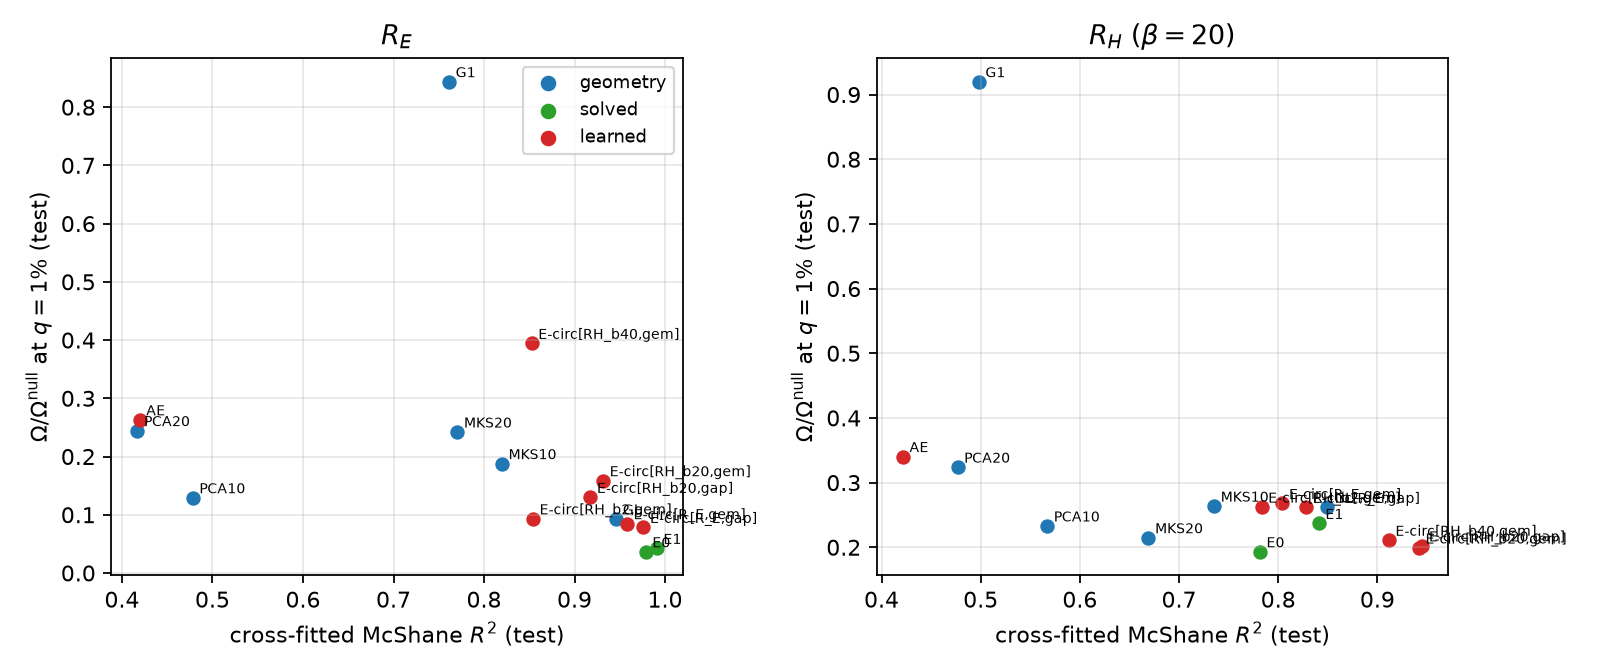
\includegraphics[width=0.92\textwidth]{fig_gate_avg_vs_worst.png}
\caption{Initial gate benchmark (\texttt{test1}, $n=300$, $d_{\rm white}$): cross-fitted McShane $R^2$ vs.\ null-normalized worst-case insufficiency $\Omega/\Omega^{\rm null}$ ($q=1\%$) for $R_E$ (left) and $R_H(\beta=20)$ (right).}
\label{fig:gate_avg_vs_worst}
\end{figure}

\begin{figure}[ht!]
\centering
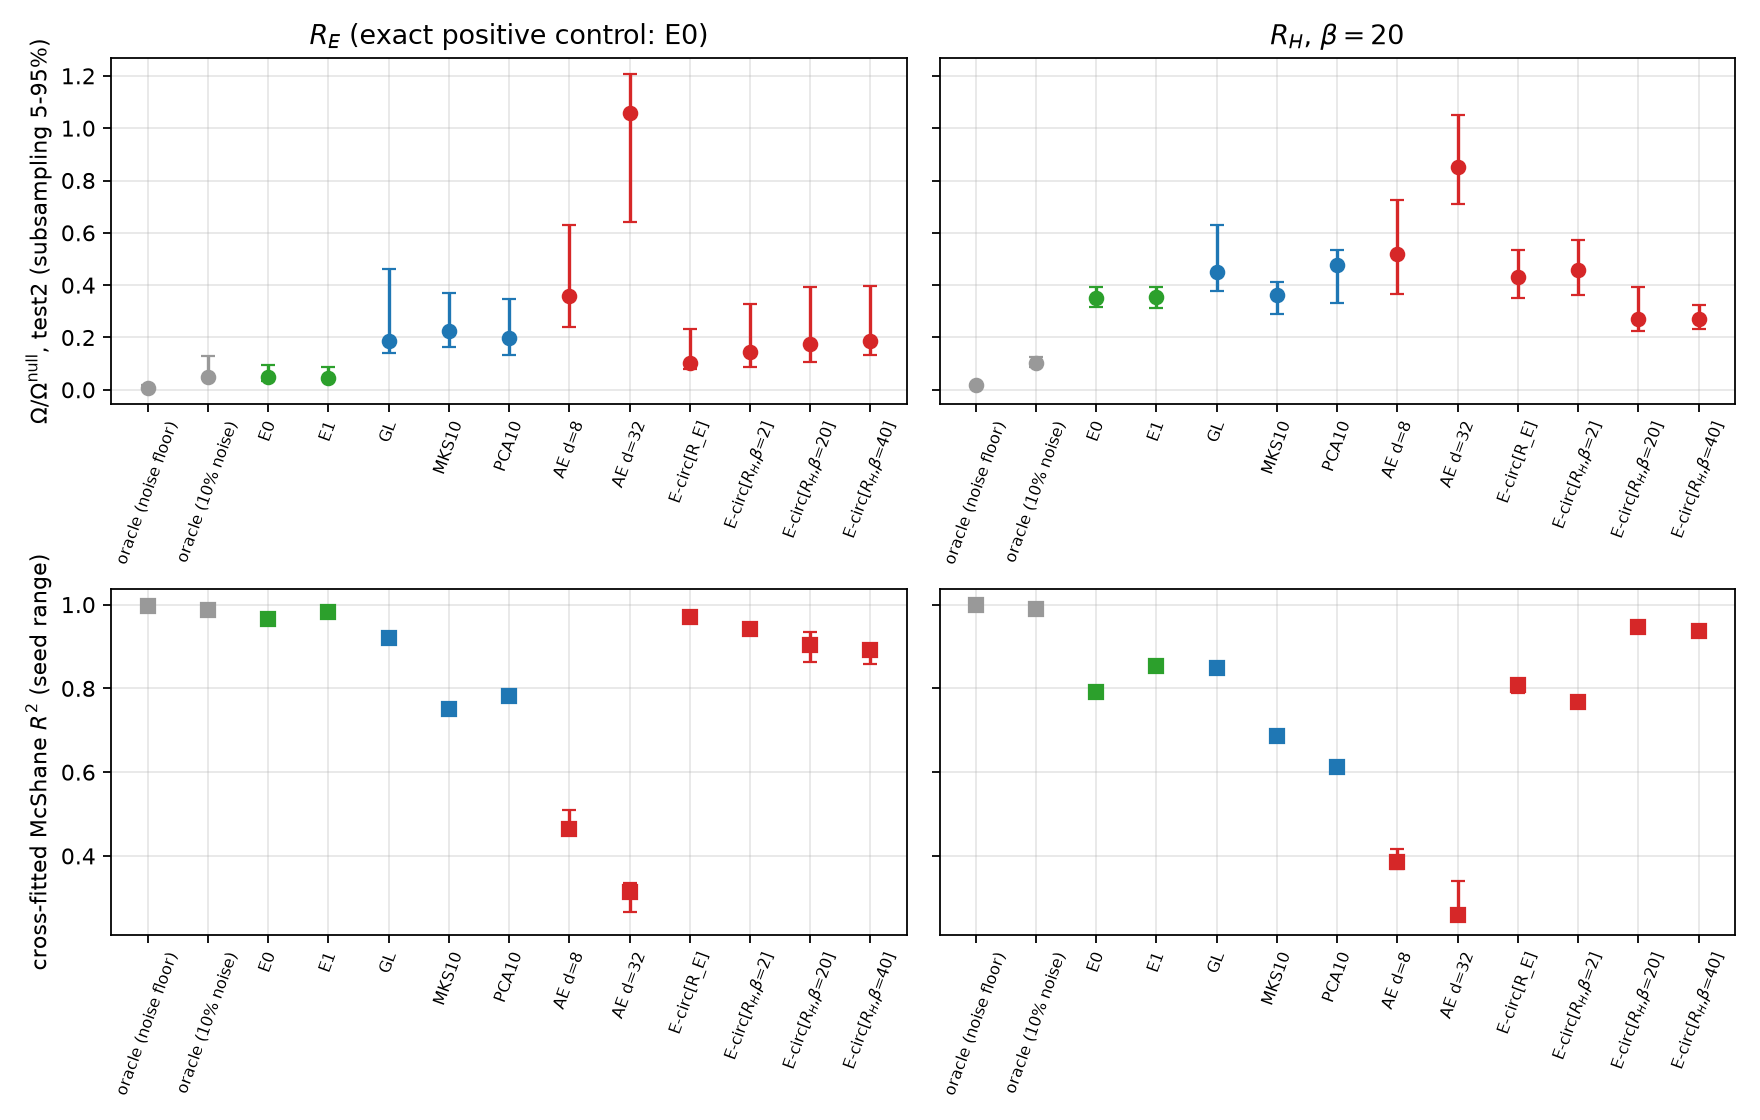
\includegraphics[width=0.95\textwidth]{fig_consolidation.png}
\caption{Consolidated 3-seed comparison (\texttt{test2}, $n=1{,}000$) showing 5--95\% paired subsampling intervals ($\text{SI}_{90}$) for $\Omega/\Omega^{\rm null}$ (top) and 3-seed min/max ranges for $R^2_{\rm McShane}$ (bottom) on $R_E$ (left) and $R_H(\beta=20)$ (right).}
\label{fig:consolidation}
\end{figure}

\subsection{Hypothesis \ref{hyp:target}: Target dependence and learnable $\GeM$ pooling exponent}

Table~\ref{tab:gem_exponent} reports the learned $\GeM_p$ pooling exponent across targets and objectives (initialized at $p_0=3.0$ with dedicated log-exponent learning rate $\eta_q=0.05$). Across the initiation hazard family $R_H(\beta)$, the 3-seed median exponent grows monotonically with tail sharpness $\beta$ from $p=3.84$ ($\beta=2$) to $p=8.64$ ($\beta=20$; $8.84\text{--}9.61$ under \texttt{SBR-CF}) and $p=10.31$ ($\beta=40$), and replacing $\GeM_p$ with fixed \texttt{GAP} ($p=1$) on $R_H(20)$ degrades \texttt{MSE} insufficiency from $0.273$ to $0.396$. On smooth bulk energy $R_E$, downstream affine layers compensate moderate power-mean distortions, leaving a flat valley around $p=3.90$, whereas removing the MSE regression head under unanchored \texttt{RNC} drives $p\to 841\text{--}2032$.

\begin{table}[ht!]
\centering
\caption{Learned generalized-mean ($\GeM_p$) pooling exponent $p$ across mechanical targets of increasing tail sharpness $\beta$ and training objectives ($d=8$, 3 seeds, initialized at $p_0=3.0$).}
\label{tab:gem_exponent}
\footnotesize
\setlength{\tabcolsep}{5.0pt}
\begin{tabular}{llcccc}
\toprule
Target & Objective & Seed 0 & Seed 1 & Seed 2 & 3-Seed Median $p$ \\
\midrule
$R_E$ (bulk homogenized energy) & \texttt{MSE} & 3.90 & 3.35 & 5.15 & 3.90 \\
$R_H(\beta=2)$ (mild heterogeneity) & \texttt{MSE} & 3.84 & 3.24 & 5.18 & \textbf{3.84} \\
$R_H(\beta=20)$ (sharp tail hazard) & \texttt{MSE} & 8.64 & 4.58 & 10.21 & \textbf{8.64} \\
$R_H(\beta=40)$ (extreme tail hazard) & \texttt{MSE} & 10.31 & 5.41 & 10.84 & \textbf{10.31} \\
\midrule
$R_H(\beta=20)$ & \texttt{SBR-CF} ($\lambda_{\rm cf}=1.0$) & 8.84 & 7.47 & 9.35 & \textbf{8.84} \\
$R_H(\beta=20)$ & \texttt{SBR-CF} ($\lambda_{\rm cf}=3.0$) & 9.61 & 8.67 & 9.78 & \textbf{9.61} \\
$R_H(\beta=20)$ & \texttt{RankSim} ($\gamma=1.0$) & 8.38 & 3.13 & 7.80 & 7.80 \\
$R_H(\beta=20)$ & \texttt{RNC} ($\tau=1.0$, no MSE head) & 841.1 & 1065.5 & 1108.8 & $1065.5^{\dagger}$ \\
$R_H(\beta=20)$ & \texttt{RNC} ($\tau=2.0$, no MSE head) & 1633.3 & 2032.4 & 1909.4 & $1909.4^{\dagger}$ \\
\bottomrule
\end{tabular}
\par\smallskip\raggedright{\footnotesize $^\dagger$Without an MSE regression head, pure \texttt{RNC} gradients drive $p\to\infty$ (hard max-pooling regime).}
\end{table}

\subsection{Experiments D--E: Cross-fitted barrier sweep, \texttt{Tail-MSE}, \texttt{SBR-in}, and matched hyperparameter selection}
\label{sec:exp_de}

To ensure transparent, symmetric hyperparameter selection across all objective families before inspecting \texttt{test2}, Table~\ref{tab:val_selection} reports the 3-seed median validation metrics on held-out $\texttt{val}$ ($n=300$, $d_{\rm white}$) across all 15 hyperparameter candidates. On $\texttt{val}$, \texttt{RankSim} selects $\gamma=1.0$ over $\gamma\in\{10,100\}$ under all three criteria ($\Omega/\Omega^{\rm null}$, ${\rm CF}_{\rm rmse}/\sigma_R$, and ${\rm CF}_{\max}/\sigma_R$); \texttt{RNC} selects $\tau=1.0$ over $\tau\in\{0.5,2.0\}$ under all three criteria; \texttt{Tail-MSE} selects $\lambda_{\rm tail}=3.0$ over $1.0$ under all three criteria; \texttt{SBR-in} selects $\lambda_{\rm bar}=1.0$ by $\Omega/\Omega^{\rm null}$ and ${\rm CF}_{\rm rmse}/\sigma_R$ (while $\lambda_{\rm bar}=3.0$ has lower $\texttt{val}\;{\rm CF}_{\max}/\sigma_R$); and within \texttt{SBR-CF}, $\lambda_{\rm cf}=1.0$ achieves the lowest validation ${\rm CF}_{\rm rmse}/\sigma_R$ ($0.186$), whereas $\lambda_{\rm cf}=3.0$ achieves the lowest validation $\Omega/\Omega^{\rm null}$ ($0.144$) and ${\rm CF}_{\max}/\sigma_R$ ($1.061$). We therefore report both $\lambda_{\rm cf}=1.0$ and $\lambda_{\rm cf}=3.0$ alongside all baseline hyperparameter settings in Table~\ref{tab:exp_de_lambda}.

\begin{table}[ht!]
\centering
\caption{Validation hyperparameter sweep on held-out \texttt{val} ($n=300$, $d=8$, 3-seed medians under $d_{\rm white}$). Bold entries mark the best hyperparameter within each multi-parameter family under each validation criterion.}
\label{tab:val_selection}
\footnotesize
\setlength{\tabcolsep}{3.5pt}
\resizebox{\textwidth}{!}{%
\begin{tabular}{llcccc}
\toprule
Method Family & Hyperparameter Grid & \texttt{val} $\Omega/\Omega^{\rm null}$ ($\downarrow$) & \texttt{val} ${\rm CF}_{\rm rmse}/\sigma_R$ ($\downarrow$) & \texttt{val} ${\rm CF}_{\max}/\sigma_R$ ($\downarrow$) & Selected Setting(s) \\
\midrule
\texttt{MSE} & $\lambda_{\rm cf}=0$ & 0.244 & 0.223 & 0.799 & $\lambda_{\rm cf}=0$ (ref.) \\
\texttt{SBR-CF} & $\lambda_{\rm cf}\in\{0.1, 0.3, 1.0, 3.0\}$ & $0.213, 0.211, 0.158, \mathbf{0.144}$ & $0.232, 0.221, \mathbf{0.186}, 0.193$ & $1.164, 1.064, 1.089, \mathbf{1.061}$ & $\lambda_{\rm cf}=1.0, 3.0$ \\
\texttt{Tail-MSE} & $\lambda_{\rm tail}\in\{1.0, 3.0\}$ & $0.228, \mathbf{0.188}$ & $0.264, \mathbf{0.260}$ & $1.230, \mathbf{1.220}$ & $\lambda_{\rm tail}=3.0$ \\
\texttt{SBR-in} & $\lambda_{\rm bar}\in\{1.0, 3.0\}$ & $\mathbf{0.238}, 0.253$ & $\mathbf{0.286}, 0.294$ & $1.243, \mathbf{1.058}$ & $\lambda_{\rm bar}=1.0, 3.0$ \\
\texttt{RankSim} & $\gamma\in\{1.0, 10.0, 100.0\}$ & $\mathbf{0.220}, 0.276, 0.237$ & $\mathbf{0.265}, 0.293, 0.288$ & $\mathbf{0.953}, 1.219, 1.157$ & $\gamma=1.0$ \\
\texttt{RNC} & $\tau\in\{0.5, 1.0, 2.0\}$ & $0.226, \mathbf{0.206}, 0.273$ & $0.311, \mathbf{0.266}, 0.288$ & $1.206, \mathbf{0.900}, 1.243$ & $\tau=1.0$ \\
\bottomrule
\end{tabular}%
}
\end{table}

Because $\Omega_\Psi(q)$ is an extreme-value order statistic over $\binom{m}{2}$ pairs, we quantify paired finite-sample stability on \texttt{test2} ($n=1{,}000$) by drawing $B=300$ paired random half-samples of size $m=500$ without replacement and recording the empirical 5th--95th percentile range $[q_5,q_{95}]$ of the seed-median difference $\Delta_{\rm paired}=\Omega_{\rm method}/\Omega_{\rm method}^{\rm null}-\Omega_{\rm MSE}/\Omega_{\rm MSE}^{\rm null}$. Because overlapping half-samples of a fixed $n=1{,}000$ test set are positively correlated, we denote $[q_5,q_{95}]$ explicitly as a $90\%$ paired Subsample Interval ($90\%\text{ SI}$), distinguishing it from an asymptotic population confidence interval.

\begin{table}[ht!]
\centering
\caption{Experiments D--E on $R_H(\beta=20)$ ($d=8$, 3-seed medians under $d_{\rm white}$, all trained for 60 epochs): comparison of \texttt{SBR-CF} against \texttt{MSE}, top-$k$ extreme-residual \texttt{Tail-MSE} ($\lambda_{\rm tail}\in\{1,3\}$), un-cross-fitted \texttt{SBR-in} ($\lambda_{\rm bar}\in\{1,3\}$), \texttt{RankSim}, and \texttt{RNC}. $\Delta_{\rm paired}$ reports the median and $90\%$ paired subsample interval ($[q_5,q_{95}]$, $90\%\text{ SI}$) over 300 paired half-samples ($m=500$) relative to \texttt{MSE}.}
\label{tab:exp_de_lambda}
\footnotesize
\setlength{\tabcolsep}{2.8pt}
\resizebox{\textwidth}{!}{%
\begin{tabular}{lcccccccc}
\toprule
Objective ($d=8$, 60 epochs) & \multicolumn{6}{c}{IID Test (\texttt{test2}, $n=1{,}000$, $d_{\rm white}$)} & \multicolumn{2}{c}{OOD (\texttt{ood}, $n=300$)} \\
\cmidrule(lr){2-7}\cmidrule(lr){8-9}
 & $\Omega/\Omega^{\rm null}$ & $\Delta_{\rm paired}$ $[90\%\text{ SI}]$ & $\%<\text{MSE}$ & $R^2_{\rm Mc}$ & $R^2_{\rm ridge}$ & ${\rm CF}_{\max}/\sigma_R$ & $\Omega/\Omega^{\rm null}$ & $R^2_{\rm Mc}$ \\
\midrule
\texttt{MSE} ($\lambda_{\rm cf}=0$) & 0.273 & $0.000$ (sub.\ 0.275) & --- & 0.947 & 0.969 & 1.677 & 0.229 & 0.957 \\
\texttt{SBR-CF} ($\lambda_{\rm cf}=0.1$) & 0.269 & $-0.033\;[-0.117,+0.035]$ & $82.3\%$ & 0.948 & 0.964 & 1.504 & 0.241 & 0.938 \\
\texttt{SBR-CF} ($\lambda_{\rm cf}=0.3$) & 0.268 & $-0.046\;[-0.178,+0.139]$ & $81.7\%$ & 0.951 & 0.970 & 1.683 & 0.216 & 0.962 \\
\texttt{SBR-CF} ($\lambda_{\rm cf}=1.0$)$^\star$ & \textbf{0.192} & $\mathbf{-0.092}\;[-0.199,-0.015]$ & $\mathbf{98.3\%}$ & \textbf{0.962} & 0.975 & 1.402 & 0.199 & \textbf{0.963} \\
\texttt{SBR-CF} ($\lambda_{\rm cf}=3.0$)$^\star$ & \textbf{0.188} & $\mathbf{-0.090}\;[-0.213,-0.025]$ & $\mathbf{99.7\%}$ & 0.961 & \textbf{0.977} & \textbf{1.165} & \textbf{0.169} & \textbf{0.963} \\
\midrule
\texttt{Tail-MSE} ($\lambda_{\rm tail}=1.0$, top-$k$) & 0.306 & $+0.021\;[-0.088,+0.114]$ & $36.0\%$ & 0.935 & 0.974 & 1.572 & 0.229 & 0.953 \\
\texttt{Tail-MSE} ($\lambda_{\rm tail}=3.0$, top-$k$)$^\star$ & 0.240 & $-0.034\;[-0.142,+0.048]$ & $74.3\%$ & 0.941 & 0.979 & 1.797 & 0.183 & 0.950 \\
\texttt{SBR-in} ($\lambda_{\rm bar}=1.0$) & 0.303 & $+0.037\;[-0.095,+0.105]$ & $26.7\%$ & 0.926 & 0.961 & 1.775 & 0.228 & 0.943 \\
\texttt{SBR-in} ($\lambda_{\rm bar}=3.0$) & 0.314 & $+0.044\;[-0.081,+0.132]$ & $21.3\%$ & 0.909 & 0.949 & 1.779 & 0.263 & 0.902 \\
\midrule
\texttt{RankSim} ($\gamma=10$, default) & 0.294 & $+0.036\;[-0.087,+0.125]$ & $26.7\%$ & 0.911 & 0.962 & 1.621 & 0.232 & 0.886 \\
\texttt{RankSim} ($\gamma=1.0$, val-selected)$^\star$ & 0.261 & $-0.012\;[-0.147,+0.045]$ & $59.0\%$ & 0.924 & 0.974 & 1.598 & 0.205 & 0.949 \\
\texttt{RNC} ($\tau=2.0$, default) & 0.298 & $+0.002\;[-0.102,+0.072]$ & $47.7\%$ & 0.903 & 0.989 & 1.797 & 0.328 & 0.893 \\
\texttt{RNC} ($\tau=1.0$, val-selected)$^\star$ & 0.225 & $-0.036\;[-0.165,+0.018]$ & $89.0\%$ & 0.915 & \textbf{0.990} & 2.065 & 0.284 & 0.915 \\
\bottomrule
\end{tabular}%
}
\par\smallskip\raggedright{\footnotesize $^\star$Selected on held-out \texttt{val} ($n=300$, Table~\ref{tab:val_selection}): $\lambda_{\rm cf}=1.0$ minimizes validation ${\rm CF}_{\rm rmse}/\sigma_R$, while $\lambda_{\rm cf}=3.0$ minimizes validation $\Omega/\Omega^{\rm null}$ and ${\rm CF}_{\max}/\sigma_R$.}
\end{table}

Table~\ref{tab:exp_de_lambda} isolates the mechanism of \texttt{SBR-CF}:
(i)~Penalizing the top-$k=16$ squared residuals of the parametric head directly (\texttt{Tail-MSE}) improves linear ridge fit ($R^2_{\rm ridge}=0.979$ at $\lambda_{\rm tail}=3.0$) and lowers $\Omega/\Omega^{\rm null}$ modestly to $0.240$, but degrades $R^2_{\rm McShane}$ ($0.947\to 0.941$) and inflates out-of-sample McShane maximum error to ${\rm CF}_{\max}/\sigma_R=1.797$. Thus emphasizing extreme head residuals is not equivalent to regularizing cross-fitted McShane neighborhoods.
(ii)~Increasing the un-cross-fitted in-sample barrier weight from $\lambda_{\rm bar}=1.0$ to $3.0$ (\texttt{SBR-in}) further worsens $\Omega/\Omega^{\rm null}$ ($0.303\to 0.314$) and $R^2_{\rm McShane}$ ($0.926\to 0.909$), confirming Section~\ref{sec:insample}.
(iii)~\texttt{SBR-CF} ($\lambda_{\rm cf}=1.0, 3.0$) cuts whitened $\Omega/\Omega^{\rm null}$ to $\mathbf{0.192}$ and $\mathbf{0.188}$ ($98.3\%\text{--}99.7\%$ paired subsample wins over \texttt{MSE}), raises $R^2_{\rm McShane}$ to $\mathbf{0.962}$, and lowers ${\rm CF}_{\max}/\sigma_R$ to $\mathbf{1.165}$ on \texttt{test2} and $\Omega/\Omega^{\rm null}$ to $\mathbf{0.169}$ on \texttt{ood\_morphology}.

\subsection{Full exact barrier curves $e^\star_\theta(\Lambda)/\sigma_R$, $\Lambda_{\rm interp}/\sigma_R$, and certified head decomposition}
\label{sec:barrier_curves}

In Table~\ref{tab:cert_floor}, post-hoc spectrally normalized Lipschitz heads $g_\phi$ are evaluated at their validation-selected dimensionless budget $\widetilde\Lambda_{\rm cert}=\Lambda_{\rm cert}/\sigma_R$. Because $\widetilde\Lambda_{\rm cert}=4.0$ exceeds the finite-sample training interpolation constant $\Lambda_{\rm interp}/\sigma_R$ in $d_{\mathcal N}$ for well-conditioned $d=8$ models (e.g., $\Lambda_{\rm interp}/\sigma_R=3.700<4.0$ for \texttt{MSE} and $2.797<4.0$ for \texttt{SBR-CF} $\lambda_{\rm cf}=1.0$ on $\texttt{train}$ in Table~\ref{tab:barrier_curves_full}), $e^\star_{\rm train}(4\sigma_R)=0$ in Table~\ref{tab:cert_floor}, so $\Delta_{\rm head}=e_{\infty,{\rm train}}$ at that budget measures the improvement in maximum training fit of the Lipschitz head ($0.513\to 0.248$). To compare the predictor-independent representation barriers $e^\star_\theta(\Lambda)$ directly across budgets where the barriers are strictly positive, Table~\ref{tab:barrier_curves_full} reports the complete exact barrier curves $e^\star_\theta(\Lambda)/\sigma_R$ across $\Lambda/\sigma_R\in\{0.25,0.5,1.0,1.5,2.0,3.0,4.0\}$ together with $\Lambda_{\rm interp}/\sigma_R$ on both $\texttt{train}$ ($n=1{,}400$) and $\texttt{test2}$ ($n=1{,}000$) in $d_{\mathcal N}$ and $d_{\rm white}$.

\begin{table}[ht!]
\centering
\caption{Exact finite-sample Lipschitz barrier curves $e^\star_\theta(\Lambda)/\sigma_R$ and finite-sample interpolation slopes $\Lambda_{\rm interp}/\sigma_R$ (Eq.~\eqref{eq:lambda_interp}) across common Lipschitz budgets $\Lambda/\sigma_R\in\{0.25,0.5,1.0,1.5,2.0,3.0,4.0\}$ on $R_H(\beta=20)$ ($d=8$, 3-seed medians) in frozen \texttt{LatentNorm} space $d_{\mathcal N}$ and full Mahalanobis whitening $d_{\rm white}$ ($\delta=10^{-9}$). Bold entries mark the exact column minimum within each split and metric space. Under $d_{\rm white}$ on \texttt{test2}, \texttt{RNC} ($\tau=1.0$) and \texttt{Tail-MSE} ($\lambda_{\rm tail}=3.0$) achieve lower positive barriers than \texttt{SBR-CF}, whereas in $d_{\mathcal N}$ on \texttt{test2}, \texttt{SBR-CF} ($\lambda_{\rm cf}=3.0$) achieves the lowest barrier at higher budgets $\Lambda/\sigma_R\in\{2.0,3.0\}$.}
\label{tab:barrier_curves_full}
\footnotesize
\setlength{\tabcolsep}{3.2pt}
\resizebox{\textwidth}{!}{%
\begin{tabular}{llcccccccc}
\toprule
Split / Space & Objective ($d=8$) & $\Lambda_{\rm interp}/\sigma_R$ & \multicolumn{7}{c}{Exact Sample Barrier $e^\star_\theta(\Lambda)/\sigma_R$ at $\Lambda/\sigma_R=$} \\
\cmidrule(lr){4-10}
 & & & $0.25$ & $0.50$ & $1.00$ & $1.50$ & $2.00$ & $3.00$ & $4.00$ \\
\midrule
\texttt{train} ($d_{\mathcal N}$)
 & \texttt{MSE} ($\lambda_{\rm cf}=0$) & 3.700 & 3.040 & 2.724 & 2.122 & 1.520 & 0.937 & 0.237 & \textbf{0.000} \\
 & \texttt{Tail-MSE} ($\lambda_{\rm tail}=3.0$) & 3.044 & 2.989 & 2.597 & 1.869 & 1.148 & 0.427 & 0.003 & \textbf{0.000} \\
 & \texttt{SBR-in} ($\lambda_{\rm bar}=1.0$) & 3.960 & 3.068 & 2.762 & 2.182 & 1.664 & 1.115 & 0.255 & \textbf{0.000} \\
 & \texttt{SBR-in} ($\lambda_{\rm bar}=3.0$) & 4.364 & 3.077 & 2.762 & 2.212 & 1.663 & 1.143 & 0.331 & 0.150 \\
 & \texttt{RankSim} ($\gamma=1.0$) & 3.356 & 3.055 & 2.690 & 2.028 & 1.400 & 0.785 & 0.024 & \textbf{0.000} \\
 & \texttt{RNC} ($\tau=1.0$) & 4.769 & \textbf{2.666} & \textbf{1.913} & \textbf{0.571} & \textbf{0.244} & \textbf{0.172} & 0.086 & 0.035 \\
 & \texttt{SBR-CF} ($\lambda_{\rm cf}=1.0$) & \textbf{2.797} & 3.094 & 2.768 & 2.117 & 1.465 & 0.842 & \textbf{0.000} & \textbf{0.000} \\
 & \texttt{SBR-CF} ($\lambda_{\rm cf}=3.0$) & 3.650 & 3.048 & 2.677 & 1.987 & 1.324 & 0.662 & 0.013 & \textbf{0.000} \\
\midrule
\texttt{test2} ($d_{\mathcal N}$)
 & \texttt{MSE} ($\lambda_{\rm cf}=0$) & 4.249 & 2.554 & 2.252 & 1.706 & 1.189 & 0.777 & 0.267 & 0.037 \\
 & \texttt{Tail-MSE} ($\lambda_{\rm tail}=3.0$) & \textbf{3.719} & 2.492 & 2.132 & 1.455 & 0.863 & 0.477 & 0.180 & \textbf{0.000} \\
 & \texttt{SBR-in} ($\lambda_{\rm bar}=1.0$) & 5.006 & 2.560 & 2.266 & 1.730 & 1.213 & 0.810 & 0.288 & 0.086 \\
 & \texttt{SBR-in} ($\lambda_{\rm bar}=3.0$) & 4.563 & 2.563 & 2.277 & 1.768 & 1.283 & 0.855 & 0.305 & 0.080 \\
 & \texttt{RankSim} ($\gamma=1.0$) & 4.531 & 2.552 & 2.229 & 1.672 & 1.217 & 0.885 & 0.340 & 0.067 \\
 & \texttt{RNC} ($\tau=1.0$) & 32.242 & \textbf{2.261} & \textbf{1.632} & \textbf{0.992} & \textbf{0.859} & 0.802 & 0.688 & 0.573 \\
 & \texttt{SBR-CF} ($\lambda_{\rm cf}=1.0$) & 4.398 & 2.571 & 2.251 & 1.632 & 1.068 & 0.584 & 0.148 & 0.034 \\
 & \texttt{SBR-CF} ($\lambda_{\rm cf}=3.0$) & 5.255 & 2.562 & 2.233 & 1.610 & 1.016 & \textbf{0.444} & \textbf{0.059} & 0.024 \\
\midrule
\texttt{test2} ($d_{\rm white}$)
 & \texttt{MSE} ($\lambda_{\rm cf}=0$) & 3.865 & 2.554 & 2.255 & 1.692 & 1.242 & 0.812 & 0.307 & \textbf{0.000} \\
 & \texttt{Tail-MSE} ($\lambda_{\rm tail}=3.0$) & 3.822 & 2.497 & 2.138 & 1.575 & 1.106 & 0.652 & 0.123 & \textbf{0.000} \\
 & \texttt{SBR-in} ($\lambda_{\rm bar}=1.0$) & 4.768 & 2.560 & 2.265 & 1.743 & 1.235 & 0.803 & 0.363 & 0.069 \\
 & \texttt{RankSim} ($\gamma=1.0$) & 3.619 & 2.530 & 2.205 & 1.571 & 1.187 & 0.808 & 0.269 & \textbf{0.000} \\
 & \texttt{RNC} ($\tau=1.0$) & \textbf{3.039} & \textbf{2.438} & \textbf{2.037} & \textbf{1.481} & \textbf{0.964} & \textbf{0.546} & \textbf{0.010} & \textbf{0.000} \\
 & \texttt{SBR-CF} ($\lambda_{\rm cf}=1.0$) & 3.731 & 2.562 & 2.234 & 1.618 & 1.121 & 0.782 & 0.189 & \textbf{0.000} \\
 & \texttt{SBR-CF} ($\lambda_{\rm cf}=3.0$) & 3.571 & 2.581 & 2.271 & 1.652 & 1.188 & 0.772 & 0.163 & \textbf{0.000} \\
\bottomrule
\end{tabular}%
}
\end{table}

\begin{table}[ht!]
\centering
\caption{Post-hoc certified Lipschitz head decomposition (Eq.~\eqref{eq:floor}, 3-seed medians on $R_H(\beta=20)$, $d=8$, in standardized target units $\sigma_R$). At $\widetilde\Lambda_{\rm cert}=\Lambda_{\rm cert}/\sigma_R=4.0$, $e^\star_{\rm train}(\Lambda_{\rm cert})/\sigma_R=0$ because $\Lambda_{\rm interp}/\sigma_R < 4.0$ on $\texttt{train}$ in $d_{\mathcal N}$ (Table~\ref{tab:barrier_curves_full}), so the reduction of $\Delta_{\rm head}=e_{\infty,{\rm train}}$ from $0.513$ (\texttt{MSE}) to $0.248$ (\texttt{SBR-CF}) reflects improved uniform fit of the spectrally normalized head on the regularized embedding.}
\label{tab:cert_floor}
\footnotesize
\setlength{\tabcolsep}{3.2pt}
\begin{tabular}{lccccccc}
\toprule
Objective & Sel.\ $\widetilde\Lambda_{\rm cert}$ & Train $e^\star_\theta(\Lambda_{\rm cert})/\sigma_R$ & Train $e_\infty$ & Head Gap $\Delta_{\rm head}$ & Test RMSE & Test $\ecf(\Lambda_{\rm cert})/\sigma_R$ \\
\midrule
\texttt{MSE} ($\lambda_{\rm cf}=0$) & 4.000 & 0.000 & 0.513 & 0.513 & 0.158 & 1.751 \\
\texttt{SBR-CF} ($\lambda_{\rm cf}=0.1$) & 4.000 & 0.000 & 0.291 & 0.291 & 0.165 & 1.541 \\
\texttt{SBR-CF} ($\lambda_{\rm cf}=1.0$) & 4.000 & 0.000 & \textbf{0.248} & \textbf{0.248} & 0.124 & 1.615 \\
\texttt{SBR-in} ($\lambda_{\rm bar}=1.0$) & 4.000 & 0.000 & 0.676 & 0.676 & 0.185 & 1.806 \\
\texttt{RankSim} ($\gamma=10$) & 8.000 & 0.185 & 0.563 & 0.327 & 0.170 & 1.358 \\
\texttt{RNC} ($\tau=2.0$) & 2.000 & 0.183 & 0.354 & 0.136 & \textbf{0.106} & \textbf{1.236} \\
\bottomrule
\end{tabular}
\end{table}

Table~\ref{tab:barrier_curves_full} reveals an important distinction between the exact global sample barrier $e^\star_\theta(\Lambda)$ and the local neighborhood metrics ($\Omega/\Omega^{\rm null}$, $\ecf$) in Table~\ref{tab:exp_de_lambda}, refining the evaluation of Hypothesis~\ref{hyp:cf}:
\begin{enumerate}
    \item \textbf{Ordering under $d_{\rm white}$ vs.\ $d_{\mathcal N}$:} Under $d_{\rm white}$ on $\texttt{test2}$, \texttt{RNC} ($\tau=1.0$) achieves the lowest exact barrier across all six evaluated budgets where the barriers are positive ($\Lambda/\sigma_R\in[0.25,3.00]$ in Table~\ref{tab:barrier_curves_full}, e.g., $1.481, 0.546, 0.010$ at $\Lambda/\sigma_R=1,2,3$), and \texttt{Tail-MSE} ($\lambda_{\rm tail}=3.0$) achieves lower positive barriers ($1.575, 0.652, 0.123$) than \texttt{SBR-CF} ($\lambda_{\rm cf}=1.0$: $1.618, 0.782, 0.189$; $\lambda_{\rm cf}=3.0$: $1.652, 0.772, 0.163$), while \texttt{SBR-CF} improves consistently over standard \texttt{MSE} ($1.692, 0.812, 0.307$ for $\Lambda/\sigma_R\ge 1.0$) and un-cross-fitted \texttt{SBR-in} ($1.743, 0.803, 0.363$). In \texttt{LatentNorm} space $d_{\mathcal N}$ on $\texttt{test2}$, \texttt{RNC} dominates at small budgets $\Lambda/\sigma_R\in[0.25,1.50]$ ($0.859$ at $1.50$, vs.\ $0.863$ for \texttt{Tail-MSE} and $1.016$ for \texttt{SBR-CF} $\lambda_{\rm cf}=3.0$), whereas \texttt{SBR-CF} ($\lambda_{\rm cf}=3.0$) achieves the lowest barrier at higher budgets $\Lambda/\sigma_R\in\{2.0,3.0\}$ ($0.444$ and $0.059$, vs.\ $0.477$ and $0.180$ for \texttt{Tail-MSE} and $0.802$ and $0.688$ for \texttt{RNC}, whose interpolation slope in $d_{\mathcal N}$ reaches $\Lambda_{\rm interp}/\sigma_R=32.24$). On $\texttt{train}$ in $d_{\mathcal N}$, \texttt{SBR-CF} ($\lambda_{\rm cf}=1.0$) achieves the lowest zero-barrier interpolation threshold $\Lambda_{\rm interp}/\sigma_R=\mathbf{2.797}$.
    \item \textbf{Why $\Omega/\Omega^{\rm null}$, $\ecf$, and $e^\star_\theta(\Lambda)$ rank models differently:} By Theorem~\ref{thm:barrier}, the exact barrier $e^\star_\theta(\Lambda)$ is governed by a single global worst-case pair $(i,j)$ at a fixed slope budget $\Lambda$, whereas $\Omega_\Psi(q)/\Omega_\Psi^{\rm null}(q)$ measures worst-case collisions restricted to the $q=1\%$ closest pairs relative to the distance distribution, and $\ecf$ measures anchor-to-query midpoint extension from $\texttt{train}$ to $\texttt{test2}$. \texttt{Tail-MSE} directly penalizes the largest individual head residuals, which separates the single most extreme global outlier pair at moderate $\Lambda$ without preventing $1\%$-ball nearest-neighbor collisions ($\Omega/\Omega^{\rm null}=0.240$) or out-of-sample McShane spikes (${\rm CF}_{\max}/\sigma_R=1.797$). Consequently, Hypothesis~\ref{hyp:cf} is \emph{partially supported}: \texttt{SBR-CF} improves $\Omega/\Omega^{\rm null}$, $R^2_{\rm McShane}$, ${\rm CF}_{\max}/\sigma_R$, certified head excess $\Delta_{\rm head}$, and high-budget barriers in $d_{\mathcal N}$, whereas exact barriers $e^\star_\theta(\Lambda)$ under $d_{\rm white}$ favor \texttt{RNC} and \texttt{Tail-MSE}.
\end{enumerate}

\subsection{Latent dimension sweep ($d\in\{4,8,16\}$) and whitening/metric sensitivity (\texttt{RNC} vs.\ \texttt{SBR-CF})}
\label{sec:dim_sweep}
\label{sec:metric_sensitivity}

Table~\ref{tab:dim_sweep} and Figure~\ref{fig:lambda_dim_sweep} evaluate \texttt{MSE} and \texttt{SBR-CF} ($\lambda_{\rm cf}=1.0$) across latent dimensions $d\in\{4,8,16\}$. Under standard \texttt{MSE}, linear ridge accuracy remains invariant ($R^2_{\rm ridge}=0.961\to 0.969\to 0.967$), showing that functional predictive information is preserved as $d$ grows; however, isotropic Mahalanobis whitening $d_{\rm white}$ amplifies weakly constrained extra coordinates at $d=16$, degrading $\Omega/\Omega^{\rm null}$ from $0.273$ to $0.433$ and $R^2_{\rm McShane}$ from $0.947$ to $0.834$ (the exact neural analogue of $E_B$ in the synthetic pilot of Section~\ref{sec:pilot}). \texttt{SBR-CF} mitigates this high-dimensional whitening dilution, cutting $\Omega/\Omega^{\rm null}$ at $d=16$ from $0.433$ to $\mathbf{0.238}$ ($100.0\%$ of paired $m=500$ subsamples below \texttt{MSE}; $R^2_{\rm McShane}=0.910$ vs.\ $0.834$) and OOD $\Omega/\Omega^{\rm null}$ from $0.336$ to $\mathbf{0.140}$.

\begin{table}[ht!]
\centering
\caption{Latent dimension sweep $d\in\{4,8,16\}$ on $R_H(\beta=20)$ (3-seed medians under $d_{\rm white}$). Standard \texttt{MSE} preserves $R^2_{\rm ridge}\approx 0.96\text{--}0.97$ while suffering isotropic whitening dilution at $d=16$ ($\Omega/\Omega^{\rm null}=0.433$); \texttt{SBR-CF} improves metric regularity at every dimension.}
\label{tab:dim_sweep}
\footnotesize
\setlength{\tabcolsep}{3.4pt}
\begin{tabular}{clccccccc}
\toprule
$d$ & Objective & \multicolumn{5}{c}{IID Test (\texttt{test2}, $n=1{,}000$)} & \multicolumn{2}{c}{OOD (\texttt{ood}, $n=300$)} \\
\cmidrule(lr){3-7}\cmidrule(lr){8-9}
 & & $\Omega/\Omega^{\rm null}$ (sub.) & $\Delta_{\rm paired}$ $[90\%\text{ SI}]$ & $\%<\text{MSE}$ & $R^2_{\rm Mc}$ & $R^2_{\rm ridge}$ & $\Omega/\Omega^{\rm null}$ & $R^2_{\rm Mc}$ \\
\midrule
4 & \texttt{MSE} & 0.301 (0.238) & $0.000$ & --- & 0.968 & 0.961 & 0.206 & 0.968 \\
4 & \texttt{SBR-CF} ($\lambda_{\rm cf}=1$) & \textbf{0.218} (\textbf{0.173}) & $-0.064\;[-0.173,+0.040]$ & $84.3\%$ & \textbf{0.980} & \textbf{0.973} & \textbf{0.173} & 0.963 \\
\midrule
8 & \texttt{MSE} & 0.273 (0.275) & $0.000$ & --- & 0.947 & 0.969 & 0.229 & 0.957 \\
8 & \texttt{SBR-CF} ($\lambda_{\rm cf}=1$) & \textbf{0.192} (\textbf{0.190}) & $\mathbf{-0.092}\;[-0.199,-0.015]$ & $\mathbf{98.3\%}$ & \textbf{0.962} & \textbf{0.975} & \textbf{0.199} & \textbf{0.963} \\
\midrule
16 & \texttt{MSE} & 0.433 (0.422) & $0.000$ & --- & 0.834 & 0.967 & 0.336 & 0.834 \\
16 & \texttt{SBR-CF} ($\lambda_{\rm cf}=1$) & \textbf{0.238} (\textbf{0.239}) & $\mathbf{-0.181}\;[-0.313,-0.106]$ & $\mathbf{100.0\%}$ & \textbf{0.910} & \textbf{0.971} & \textbf{0.140} & \textbf{0.899} \\
\bottomrule
\end{tabular}
\end{table}

\begin{figure}[ht!]
\centering
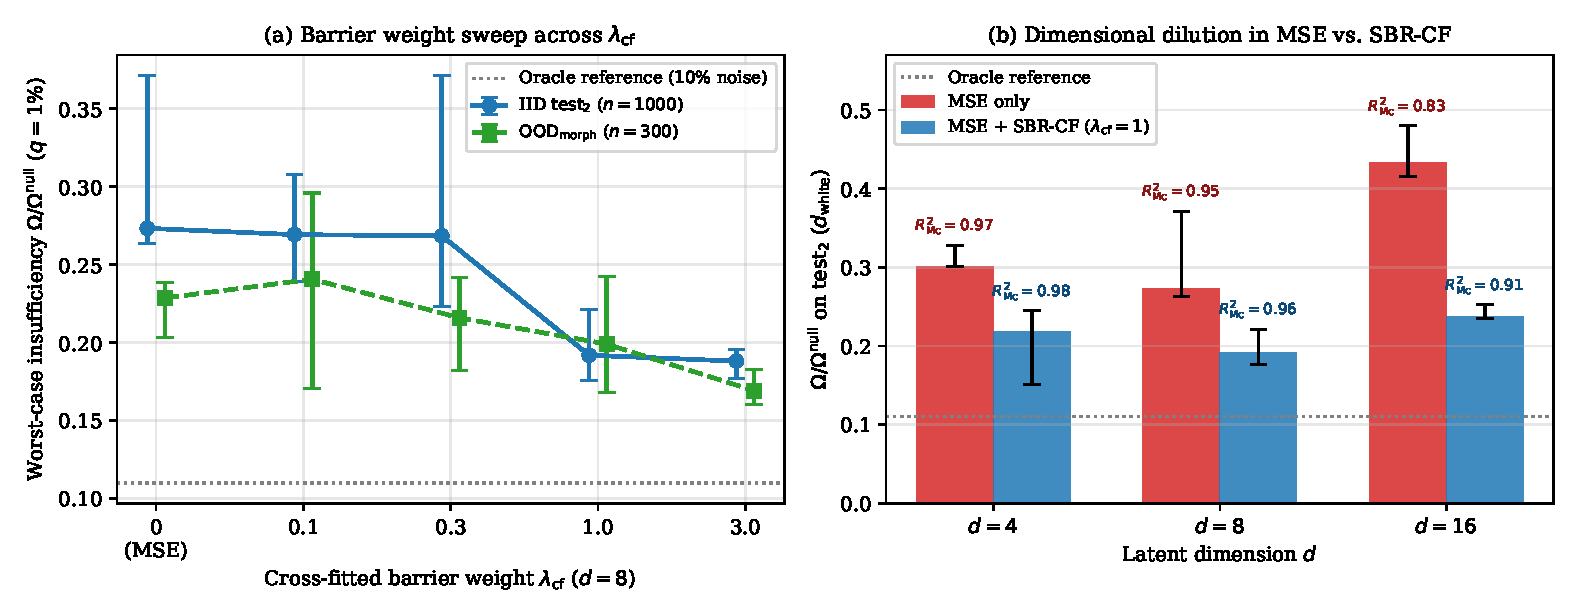
\includegraphics[width=0.98\textwidth]{fig_lambda_and_dim_sweep.pdf}
\caption{Left: Full-sample 3-seed median and min/max range of $\Omega/\Omega^{\rm null}$ on \texttt{test2} ($n=1{,}000$) and \texttt{ood\_morphology} ($n=300$) across $\lambda_{\rm cf}\in\{0,0.1,0.3,1.0,3.0\}$. Right: Dimensional sweep $d\in\{4,8,16\}$ under $d_{\rm white}$.}
\label{fig:lambda_dim_sweep}
\end{figure}

To provide a balanced, comprehensive comparison between \texttt{SBR-CF} and Rank-N-Contrast (\texttt{RNC}), Table~\ref{tab:ablation7_metrics} and Figure~\ref{fig:ablation7_metrics} evaluate all methods across the five metric normalizations of Section~\ref{sec:metric}: full Mahalanobis whitening $d_{\rm white}$ ($\delta=10^{-9}$, Eq.~\eqref{eq:white-distance}), trace-scaled regularized whitening $d_{\rm reg}(\alpha_{\rm reg})$ across $\alpha_{\rm reg}\in\{10^{-5},10^{-3},10^{-2},10^{-1}\}$ and validation-selected $d_{\rm reg}^\star$ (Eq.~\eqref{eq:dreg}), eigenvalue-truncated whitening $d_{\rm trunc}$ ($\lambda_k\ge 10^{-2}\lambda_1$), exact training-set coordinate standardization $d_{\rm std}$, and frozen \texttt{LatentNorm} running-moment standardization $d_{\mathcal N}$.

\begin{table}[ht!]
\centering
\caption{Metric and whitening regularization sensitivity on \texttt{test2} ($n=1{,}000$, $d=8$, 3-seed medians) across full whitening $d_{\rm white}$ ($\delta=10^{-9}$), trace-scaled regularized whitening $d_{\rm reg}(\alpha_{\rm reg})$ ($\alpha_{\rm reg}\in\{10^{-5},10^{-3}\}$ and validation-selected $d_{\rm reg}^\star$), truncated-spectrum whitening $d_{\rm trunc}$, exact training-set coordinate standardization $d_{\rm std}$, and frozen \texttt{LatentNorm} $d_{\mathcal N}$. Participation ratio $d_{\rm eff}=(\sum_k\lambda_k)^2/\sum_k\lambda_k^2$ and top eigenvalue share $\lambda_1/\sum_k\lambda_k$ quantify embedding dimensionality.}
\label{tab:ablation7_metrics}
\footnotesize
\setlength{\tabcolsep}{2.2pt}
\resizebox{\textwidth}{!}{%
\begin{tabular}{lccccccccccccc}
\toprule
Objective ($d=8$) & $d_{\rm eff}$ & $\frac{\lambda_1}{\sum\lambda_k}$ & \multicolumn{6}{c}{$\Omega/\Omega^{\rm null}$ ($\downarrow$) on \texttt{test2}} & \multicolumn{3}{c}{$R^2_{\rm McShane}$ ($\uparrow$) on \texttt{test2}} & \multicolumn{2}{c}{${\rm CF}_{\max}/\sigma_R$ ($\downarrow$)} \\
\cmidrule(lr){4-9}\cmidrule(lr){10-12}\cmidrule(lr){13-14}
 & & & $d_{\rm white}$ & $d_{\rm reg}(10^{-5})$ & $d_{\rm reg}(10^{-3})$ & $d_{\rm reg}^\star$ & $d_{\rm trunc}$ & $d_{\rm std}$ / $d_{\mathcal N}$ & $d_{\rm white}$ & $d_{\rm reg}^\star$ & $d_{\rm std}$ & $d_{\rm white}$ & $d_{\rm std}$ \\
\midrule
\texttt{MSE} ($\lambda_{\rm cf}=0$) & 5.03 & 0.341 & 0.273 & 0.271 & 0.271 & 0.271 & 0.271 & 0.264 / 0.258 & 0.947 & 0.948 & 0.952 & 1.677 & 1.650 \\
\texttt{Tail-MSE} ($\lambda_{\rm tail}=1.0$) & 4.71 & 0.358 & 0.306 & 0.306 & 0.306 & 0.258 & 0.288 & 0.257 / 0.257 & 0.935 & 0.943 & 0.959 & 1.572 & 1.503 \\
\texttt{Tail-MSE} ($\lambda_{\rm tail}=3.0$) & 3.68 & 0.456 & 0.240 & 0.240 & 0.240 & 0.237 & 0.240 & 0.222 / 0.222 & 0.941 & 0.955 & 0.967 & 1.797 & 1.797 \\
\texttt{SBR-in} ($\lambda_{\rm bar}=1.0$) & 5.42 & 0.279 & 0.303 & 0.303 & 0.303 & 0.304 & 0.303 & 0.300 / 0.274 & 0.926 & 0.915 & 0.937 & 1.775 & 1.926 \\
\texttt{SBR-in} ($\lambda_{\rm bar}=3.0$) & 5.86 & 0.242 & 0.314 & 0.314 & 0.314 & 0.314 & 0.314 & 0.314 / 0.295 & 0.909 & 0.915 & 0.931 & 1.779 & 1.765 \\
\texttt{RankSim} ($\gamma=1.0$) & 1.32 & 0.868 & 0.261 & 0.258 & 0.258 & 0.219 & 0.266 & 0.236 / 0.237 & 0.924 & 0.957 & 0.950 & 1.598 & 1.598 \\
\texttt{RNC} ($\tau=1.0$) & 1.004 & 0.998 & 0.225 & 0.224 & 0.166 & \textbf{0.085} & 0.281 & \textbf{0.148} / \textbf{0.148}$^\dagger$ & 0.915 & \textbf{0.989} & \textbf{0.991} & 2.065 & \textbf{1.028} \\
\texttt{SBR-CF} ($\lambda_{\rm cf}=1.0$) & 5.77 & 0.283 & 0.192 & 0.193 & 0.193 & 0.193 & 0.193 & 0.192 / 0.192 & \textbf{0.962} & 0.965 & 0.976 & 1.402 & 1.520 \\
\texttt{SBR-CF} ($\lambda_{\rm cf}=3.0$) & 5.21 & 0.312 & \textbf{0.188} & \textbf{0.188} & \textbf{0.188} & 0.187 & \textbf{0.186} & 0.150 / 0.150 & 0.961 & 0.966 & 0.981 & \textbf{1.165} & 1.239 \\
\bottomrule
\end{tabular}%
}
\par\smallskip\raggedright{\footnotesize $^\dagger$As detailed in Section~\ref{sec:metric}, $d_{\rm std}$ uses exact full-training-set coordinate moments $(\mu_{\rm tr},\sigma_{\rm tr})$, whereas $d_{\mathcal N}$ uses the frozen running \texttt{BatchNorm1d} moments $(\mu_{\rm bn},\sigma_{\rm bn})$ accumulated during training forward passes; for \texttt{RNC}, both yield 3-seed medians $\Omega/\Omega^{\rm null}=0.148$, $R^2_{\rm McShane}=0.991$, and ${\rm CF}_{\max}/\sigma_R=1.028$. Under $d_{\rm reg}(10^{-5})$, \texttt{RNC} attains $R^2_{\rm McShane}=0.922$ and 3-seed median ${\rm CF}_{\max}/\sigma_R=1.527$ (seed range $[1.203,2.065]$), vs.\ $0.915$ and $2.065$ under $d_{\rm white}$ ($\delta=10^{-9}$). Across $\alpha_{\rm reg}\in\{10^{-5},10^{-3},10^{-2},10^{-1}\}$, \texttt{RNC}'s $\Omega/\Omega^{\rm null}$ moves from $0.224\to 0.166\to 0.112\to 0.085$, whereas \texttt{SBR-CF} ($\lambda_{\rm cf}=1,3$) remains within $[0.192,0.193]$ and $[0.187,0.188]$.}
\end{table}

\begin{figure}[ht!]
\centering
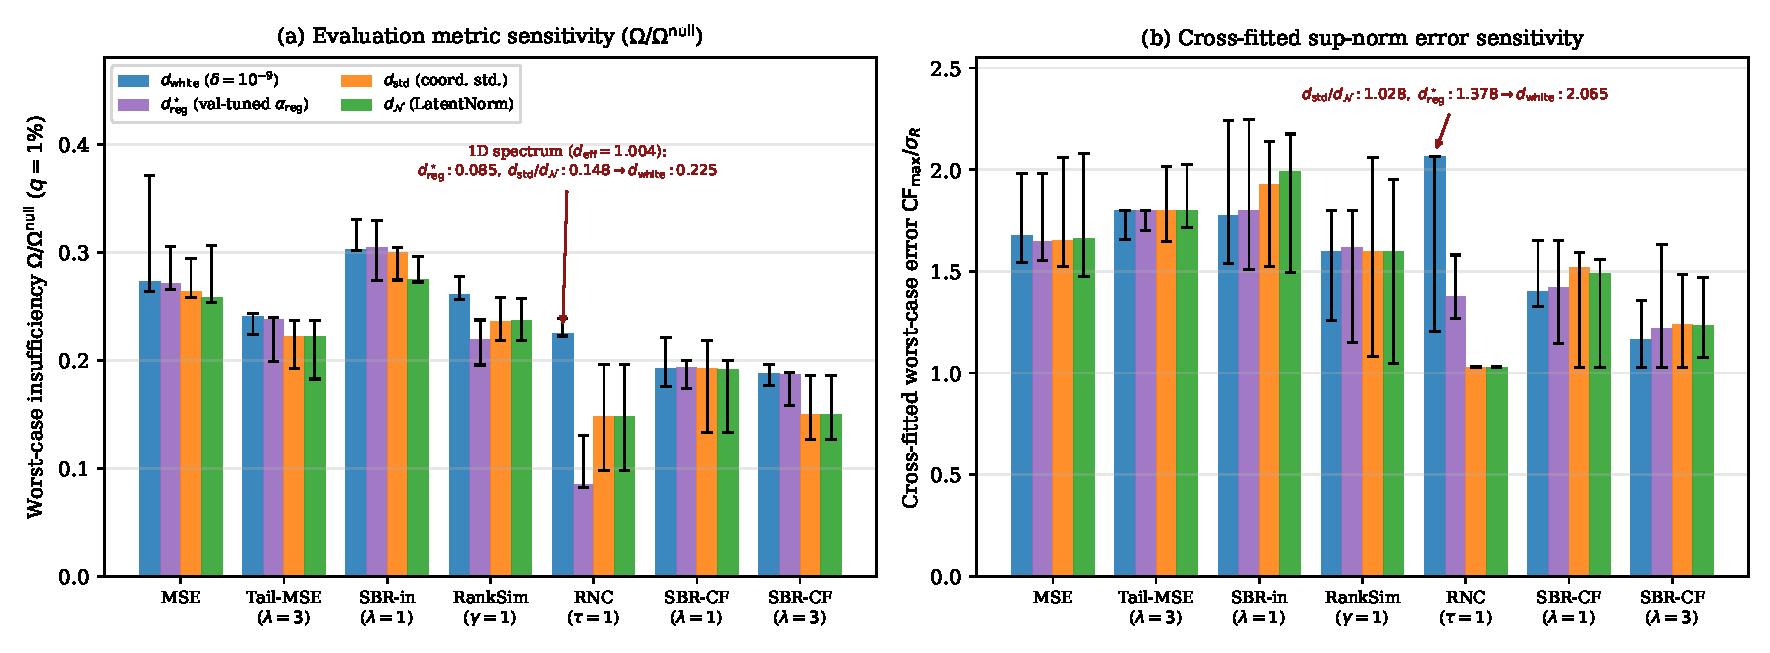
\includegraphics[width=0.98\textwidth]{fig_ablation7_metrics.pdf}
\caption{Evaluation metric sensitivity on \texttt{test2} ($d=8$; bars show 3-seed medians, whiskers give 3-seed min/max ranges) across full Mahalanobis whitening $d_{\rm white}$ ($\delta=10^{-9}$), validation-selected regularized whitening $d_{\rm reg}^\star$, coordinate standardization $d_{\rm std}$, and frozen \texttt{LatentNorm} $d_{\mathcal N}$, including both \texttt{RNC}'s $d_{\mathcal N}$ bar and the \texttt{Tail-MSE} ($\lambda=3$) baseline.}
\label{fig:ablation7_metrics}
\end{figure}

Table~\ref{tab:ablation7_metrics} and Figure~\ref{fig:ablation7_metrics} reveal a fundamental structural trade-off between 1D rank-contrastive embeddings (\texttt{RNC}) and full-rank barrier-regularized embeddings (\texttt{SBR-CF}):
\begin{enumerate}
    \item \textbf{Strengths of \texttt{RNC} under coordinate standardization and regularized whitening:} Because $R_H(\beta=20)$ is a scalar target, collapsing the 8-dimensional embedding onto a nearly one-dimensional curve ($d_{\rm eff}=1.004$, with $99.8\%$ of variance in the leading eigenvalue; recall that an ideal scalar map $E(x)=R(x)$ is 1D) is geometrically natural for single-target prediction. Under coordinate standardization $d_{\rm std}$, frozen \texttt{LatentNorm} $d_{\mathcal N}$, or validation-regularized whitening $d_{\rm reg}^\star$ ($\alpha_{\rm reg}=10^{-1}$, which downweights the 7 minor eigendirections), \texttt{RNC} ($\tau=1.0$) achieves the strongest single-target metrics in Table~\ref{tab:ablation7_metrics}: $\Omega/\Omega^{\rm null}=0.148$ ($d_{\rm std}$ and $d_{\mathcal N}$) and $0.085$ ($d_{\rm reg}^\star$), $R^2_{\rm McShane}=0.991$ and $0.989$, ${\rm CF}_{\max}/\sigma_R=1.028$, and $R^2_{\rm ridge}=0.990$.
    \item \textbf{Distinct effects of full whitening $d_{\rm white}$ vs.\ 1D spectral truncation $d_{\rm trunc}$ on \texttt{RNC}, and metric stability of \texttt{SBR-CF}:} Under full Mahalanobis whitening $d_{\rm white}$ ($\delta=10^{-9}$) or nearly unregularized $d_{\rm reg}(10^{-5})$, rescaling the 7 minor eigendirections ($\lambda_2/\lambda_1\le 3.13\times 10^{-3}$) to unit variance amplifies transverse noise, raising \texttt{RNC}'s $\Omega/\Omega^{\rm null}$ to $0.225$ ($0.224$ under $d_{\rm reg}(10^{-5})$) and increasing its cross-fitted maximum error to ${\rm CF}_{\max}/\sigma_R=2.065$ ($1.527$ median, $2.065$ max under $d_{\rm reg}(10^{-5})$). Under hard eigenvalue truncation $d_{\rm trunc}$ ($\lambda_k\ge 10^{-2}\lambda_1$), the opposite mechanism occurs: because $\lambda_2/\lambda_1<10^{-2}$, $d_{\rm trunc}$ sets $k_{\rm eff}=1$ and projects \texttt{RNC} orthogonally onto its single leading principal axis $v_1$ (discarding the 7 minor directions rather than amplifying them). This 1D projection preserves global McShane interpolation ($R^2_{\rm McShane}=0.991$, ${\rm CF}_{\max}/\sigma_R=1.278$), but increases the local $1\%$-ball collision ratio $\Omega/\Omega^{\rm null}$ to $0.281$ because projecting out small transverse separations folds nearly co-projected cells into the $q=1\%$ nearest-neighbor set. By contrast, \texttt{SBR-CF} maintains a well-conditioned multi-dimensional covariance ($d_{\rm eff}=5.77$ at $\lambda_{\rm cf}=1.0$ and $5.21$ at $\lambda_{\rm cf}=3.0$, $k_{\rm eff}=8$), yielding empirically stable insufficiency across all spectral transformations ($0.192\text{--}0.193$ across $d_{\rm white}, d_{\rm reg}(10^{-5}), d_{\rm reg}^\star, d_{\rm trunc}, d_{\rm std}, d_{\mathcal N}$ for $\lambda_{\rm cf}=1.0$; $0.186\text{--}0.188$ across whitened/truncated metrics and $0.150$ under $d_{\rm std}/d_{\mathcal N}$ for $\lambda_{\rm cf}=3.0$). As shown in Section~\ref{sec:transfer_pf}, this multi-dimensional structure also enables \texttt{SBR-CF} to transfer across distinct mechanical targets ($R_E, R_H(2)$) under whitened McShane evaluation ($d_{\rm white}$) and standalone prospective fracture (\texttt{Set C2}) where a 1D embedding specialized to $R_H(20)$ degrades.
\end{enumerate}

% ============================================================================
\section{Physical Counterexamples, Grid Convergence, and Component Ablations}
\label{sec:counterexamples_ablations}

\subsection{Experiment F: Physical counterexample pairs, collision resolution across seeds, and $254\times 254$ FFT grid refinement}
\label{sec:counterexamples}

To test Hypothesis~\ref{hyp:mech}, we inspect the exact worst-case \texttt{MSE} collision pairs at $q=1\%$ across each seed on \texttt{test2} ($\sigma_R=4.33$) and across the full ensemble of $227$ severe \texttt{MSE} collisions on \texttt{test2} (and $9$ severe collisions on \texttt{ood\_morphology}) satisfying $q_{\rm MSE}\le 1\%$ and $|\Delta R_H|$ in the top decile of $1\%$-ball pair differences ($|\Delta R_H|\ge 2.47$ on \texttt{test2}). Table~\ref{tab:counterexamples_h5} and Figure~\ref{fig:counterexample_resolution} report seed-matched and 3-seed median tracking.

To verify that these severe hazard differences $|\Delta R_H(20)|$ on the fixed voxelized masks are not artifacts of FFT or nonlocal-kernel under-resolution on the $127\times 127$ grid (where minimum gaps of $2.2\text{--}3.0$\,px span $2\text{--}3$ voxels and nonlocal averaging radius $\ell=0.025$ spans $3.18$\,px), we refine all 20 microstructures comprising the top-10 consensus \texttt{MSE} counterexample pairs onto a $2\times$ finer $254\times 254$ periodic grid by exact $2\times 2$ sub-voxel splitting (\texttt{np.repeat(..., 2)} along both axes) of the $127\times 127$ binary phase masks, re-solve the Moulinec--Suquet FFT elasticity problem at $254\times 254$ with doubled kernel resolution ($\ell=6.35$\,px), and recompute $R_E$ and $R_H(20)$. Keeping the discrete voxelized phase boundary fixed while doubling the FFT and nonlocal-averaging resolution tests the numerical stability of the FFT stress solve and nonlocal integral on the fixed pixelated geometry (note that this check does not re-rasterize smooth analytical circle/ellipse boundaries and therefore does not bound continuum boundary-discretization error).

\begin{table}[ht!]
\centering
\caption{Experiment F: resolution of physical latent counterexamples on $R_H(\beta=20)$ and $254\times 254$ FFT solver stability on the fixed voxelized masks. Top rows track each seed's exact worst-case \texttt{MSE} $\Omega(0.01)$ pair and the top-3 consensus pairs across \texttt{MSE} and \texttt{SBR-CF} ($\lambda_{\rm cf}=1,3$). Bottom rows report aggregate resolution across all $227$ severe \texttt{MSE} collisions on \texttt{test2} and $9$ severe collisions on \texttt{ood\_morphology}.}
\label{tab:counterexamples_h5}
\footnotesize
\setlength{\tabcolsep}{2.6pt}
\resizebox{\textwidth}{!}{%
\begin{tabular}{llccccccc}
\toprule
Seed / Split & Pair / Ensemble & $|\Delta R_H|_{127}$ & $|\Delta R_H|_{254}$ & $\Delta f$ & Geom.\ Contrast & \texttt{MSE} ($\lambda=0$) & \texttt{SBR-CF} ($\lambda=1$) & \texttt{SBR-CF} ($\lambda=3$) \\
 & & ($127^2$) & ($254^2$ FFT) & & (gaps / counts) & $d_{\rm white}$ ($q\%$) / Slope & $d_{\rm white}$ ($q\%$) / Slope & $d_{\rm white}$ ($q\%$) / Slope \\
\midrule
Seed 0 (\texttt{test2}) & (2401, 3205) & 5.88 & --- & 0.097 & 12 vs 9 disks (3.0\,px) & 0.403 (0.75\%) / 14.6 & \textbf{0.884} (\textbf{21.1\%}) / \textbf{6.6} & \textbf{0.870} (\textbf{16.7\%}) / \textbf{6.8} \\
Seed 1 (\texttt{test2}) & (3214, 3270) & 6.06 & --- & 0.018 & 12 vs 12 ell.\ (2.24 vs 3.0\,px) & 0.404 (0.95\%) / 15.0 & \textbf{0.724} (\textbf{11.6\%}) / \textbf{8.4} & \textbf{1.101} (\textbf{31.5\%}) / \textbf{5.5} \\
Seed 2 (\texttt{test2}) & (2981, 3270) & 8.26 & --- & 0.111 & 16 disks vs 12 ell.\ (3.0\,px) & 0.435 (0.94\%) / 19.0 & \textbf{1.143} (\textbf{37.2\%}) / \textbf{7.2} & \textbf{1.266} (\textbf{45.6\%}) / \textbf{6.5} \\
\midrule
Cons.\ \#1 & (2751, 3270) & 4.512 & 4.577 ($1.4\%$) & 0.011 & 16 disks vs 12 ell.\ (3.0\,px) & 0.333 (0.43\%) / 13.6 & \textbf{0.503} (\textbf{3.8\%}) / \textbf{9.0} & \textbf{0.651} (\textbf{8.0\%}) / \textbf{6.9} \\
Cons.\ \#2 & (2723, 3270) & 4.487 & 4.514 ($0.6\%$) & 0.036 & 16 disks vs 12 ell.\ (3.0\,px) & 0.341 (0.49\%) / 13.2 & \textbf{0.542} (\textbf{5.1\%}) / \textbf{8.3} & \textbf{0.678} (\textbf{9.4\%}) / \textbf{6.6} \\
Cons.\ \#3 & (2340, 3207) & 4.092 & 3.840 ($6.6\%$) & 0.008 & 9 disks vs 12 ell.\ (2.5\,px) & 0.352 (0.58\%) / 11.6 & \textbf{0.489} (\textbf{3.3\%}) / \textbf{8.4} & \textbf{0.612} (\textbf{6.4\%}) / \textbf{6.7} \\
\midrule
\multicolumn{9}{l}{\textit{Aggregate across all 227 severe \texttt{MSE} collisions on \texttt{test2} ($q_{\rm MSE}\le 1\%$, top 10\% $|\Delta R_H|$):}} \\
\multicolumn{6}{l}{\quad Median whitened distance $d_{\rm white}$ (median quantile $q\%$)} & 0.380 (0.60\%) & \textbf{0.412} (\textbf{2.37\%}) & \textbf{0.496} (\textbf{3.53\%}) \\
\multicolumn{6}{l}{\quad Median local Lipschitz slope $|\Delta R_H|/d_{\rm white}$} & 6.43 & \textbf{5.91} & \textbf{4.85} \\
\multicolumn{6}{l}{\quad Fraction pushed outside $q=1\%$ ball (vs.\ \texttt{SBR-in} $50.7\%$, \texttt{RankSim} $71.4\%$)} & $8.8\%^{\dagger}$ & $\mathbf{85.5\%}$ & $\mathbf{94.7\%}$ \\
\midrule
\multicolumn{9}{l}{\textit{Aggregate across all 9 severe \texttt{MSE} collisions on \texttt{ood\_morphology} ($q_{\rm MSE}\le 1\%$, top 10\% $|\Delta R_H|$):}} \\
\multicolumn{6}{l}{\quad Fraction of OOD severe collisions pushed outside $q=1\%$ ball} & $11.1\%^{\dagger}$ & $\mathbf{77.8\%}$ & $\mathbf{88.9\%}$ \\
\bottomrule
\end{tabular}%
}
\par\smallskip\raggedright{\footnotesize $^\dagger$A pair inside $q=1\%$ in one MSE seed may lie just outside $1\%$ under \texttt{MSE}'s cross-seed median embedding. Across all top-10 consensus pairs (Appendix~\ref{app:grid_conv}), the median relative change between $|\Delta R_H(20)|_{127}$ and $|\Delta R_H(20)|_{254}$ upon $2\times 2$ sub-voxel splitting is $2.55\%$ (maximum $8.13\%$).}
\end{table}

\begin{figure}[ht!]
\centering
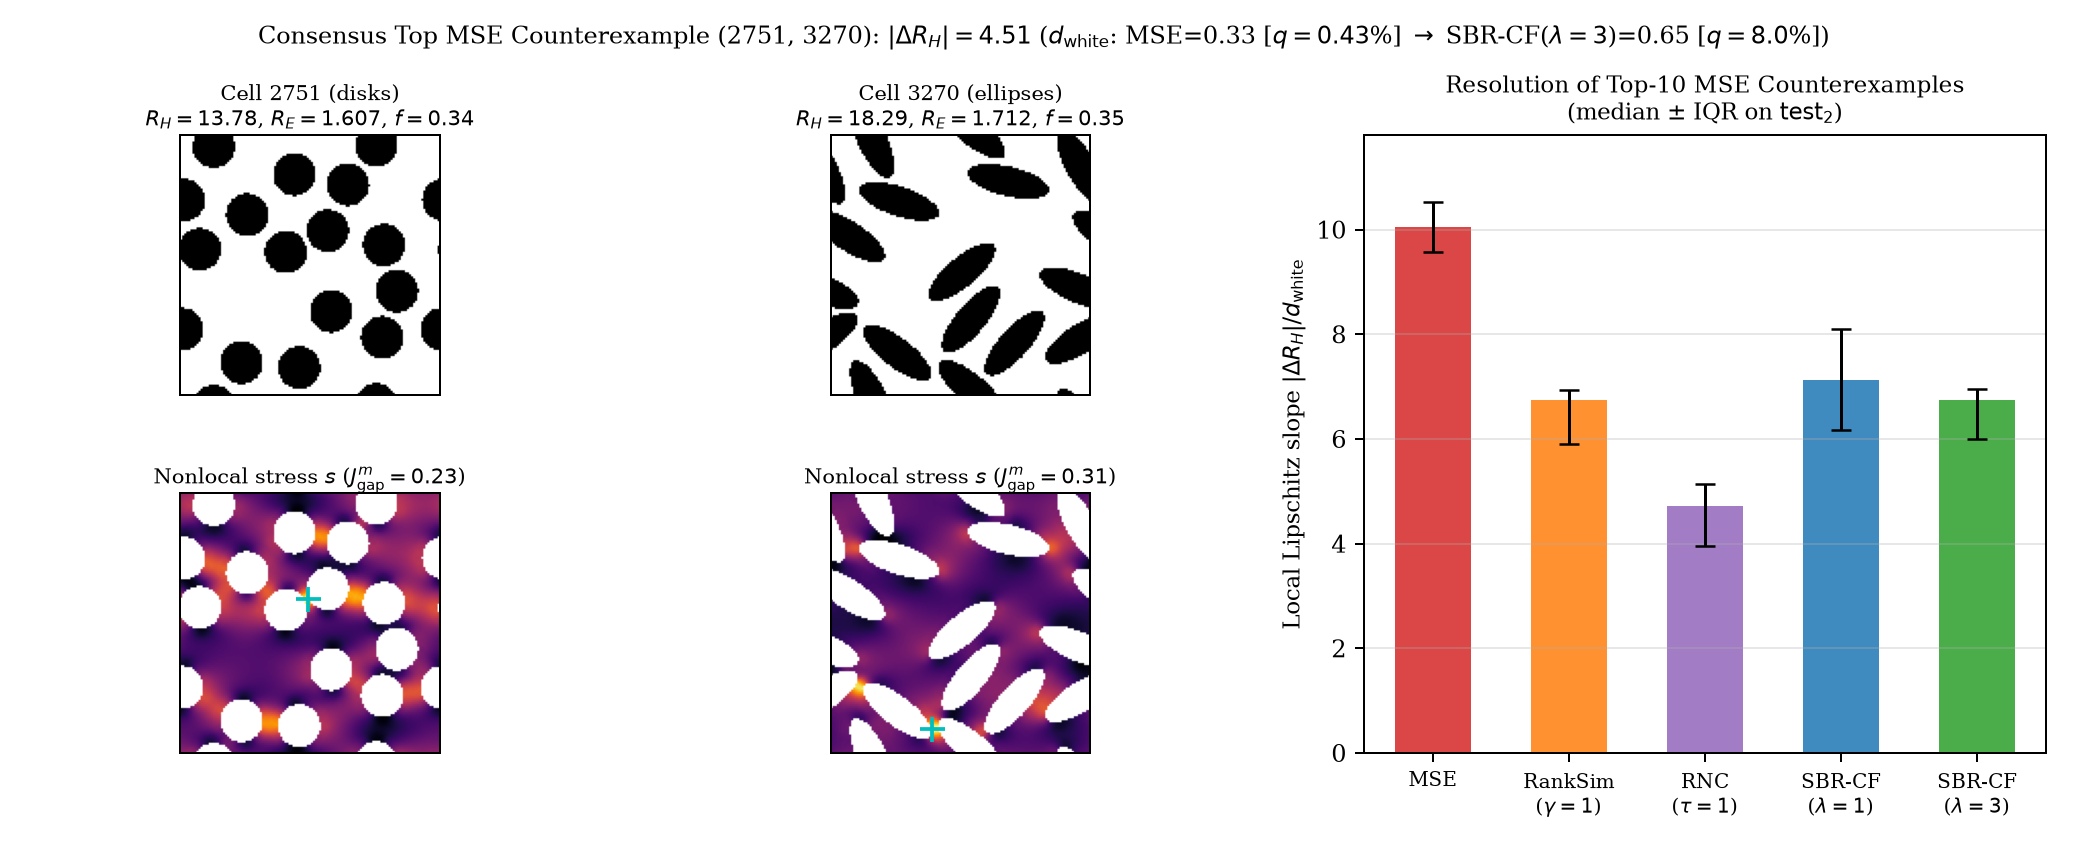
\includegraphics[width=0.98\textwidth]{fig_counterexample_resolution.png}
\caption{Physical counterexample resolution on \texttt{test2} (Experiment F, Hypothesis~\ref{hyp:mech}). Left/Center: Consensus rank-\#1 \texttt{MSE} collision pair $(2751, 3270)$, pairing a 16-disk cell ($f=0.337, R_H=13.78$ at $127^2$; $13.92$ at $254^2$) and a 12-ellipse cell ($f=0.348, R_H=18.29$ at $127^2$; $18.50$ at $254^2$, $\Delta J_{\rm gap}^m=0.081$, $|\Delta R_H|=4.51$ at $127^2$ vs.\ $4.58$ at $254^2$). Under \texttt{MSE} they collide at $d_{\rm white}=0.33$ ($q=0.43\%$, slope $13.6$), whereas \texttt{SBR-CF} ($\lambda_{\rm cf}=3$) separates them to $d_{\rm white}=0.65$ ($q=8.0\%$, slope $6.9$). Right: Top-10 \texttt{MSE} collision slopes (median $\pm$ IQR).}
\label{fig:counterexample_resolution}
\end{figure}

Table~\ref{tab:counterexamples_h5} and Appendix~\ref{app:grid_conv} confirm two points:
(i)~Across the top-10 consensus counterexample pairs, doubling the FFT resolution from $127\times 127$ to $254\times 254$ via $2\times 2$ sub-voxel splitting changes $|\Delta R_H(20)|$ by a median of $\mathbf{2.55\%}$ (maximum $8.13\%$; for the rank-\#1 pair $(2751,3270)$, $|\Delta R_H(20)|=4.512$ at $127^2$ vs.\ $4.577$ at $254^2$, a $1.42\%$ change), confirming that the computed hazard differences are numerically stable with respect to the FFT grid and nonlocal kernel resolution on the fixed voxelized geometry; and
(ii)~across all $227$ severe \texttt{MSE} collisions on \texttt{test2}, \texttt{SBR-CF} pushes $\mathbf{85.5\%}$ ($\lambda_{\rm cf}=1$) and $\mathbf{94.7\%}$ ($\lambda_{\rm cf}=3$) outside the $1\%$ nearest-neighbor ball (and $77.8\%\text{--}88.9\%$ on OOD).

\subsection{Architecture, pooling, and exploratory component ablations}
\label{sec:ablations}

To examine the roles of cross-batch anchor memory, leave-one-out hard-query mining, matched $\GeM_p$ pooling, spectral operator backbones (\texttt{E-FNO}), and built-in periodic/dihedral equivariance (\texttt{E-circ} vs.\ zero-padded \texttt{E-std}), we evaluate the 12-family, 3-seed ablation suite on $R_H(\beta=20)$ at $d=8$. In this suite, the primary objective rows (\texttt{E-circ + GeM + MSE}, \texttt{SBR-in}, and full \texttt{SBR-CF} $\lambda_{\rm cf}=1,3$) use the 60-epoch primary schedule ($\texttt{mine\_every}=1$), whereas the auxiliary ablation rows (\texttt{no mem}, \texttt{no mine}, \texttt{GAP + SBR-CF}, \texttt{E-FNO}, and \texttt{E-std}) were trained under a shorter 45-epoch schedule with $\texttt{mine\_every}=5$. Consequently, the internal 45-epoch pairs---\texttt{E-FNO} with \texttt{MSE} vs.\ \texttt{SBR-CF}, and \texttt{E-std} with vs.\ without $\mathcal L_{\rm inv}$---are strictly schedule-matched, whereas comparisons of the 45-epoch \texttt{no mem} and \texttt{no mine} rows against 60-epoch full \texttt{SBR-CF} are presented as exploratory comparisons because they vary both the ablated component and the epoch/mining schedule. In addition to sufficiency metrics, we record the empirical periodic-translation and reflection invariance defect
\begin{equation}
\delta_{\rm inv}(E_\theta)
=
\left(
\frac{1}{nd}\sum_{i=1}^n\norm{\frac{E_\theta(g\cdot x_i)-E_\theta(x_i)}{\sigma_z}}_2^2
\right)^{1/2}
\end{equation}
under shift $(17,-23)$ composed with horizontal reflection across $n=200$ \texttt{test2} cells. Table~\ref{tab:ablations_phase3} and Figure~\ref{fig:phase3_ablations} summarize the results.

\begin{table}[ht!]
\centering
\caption{Architecture, pooling, and exploratory objective-component ablations on \texttt{test2} ($n=1{,}000$) and \texttt{ood\_morphology} ($n=300$, $d=8$, 3-seed medians under $d_{\rm white}$): objective decomposition (no cross-batch memory $M=0$, no hard-query mining $K_{\rm mine}=0$), pooling (\texttt{GAP} vs.\ $\GeM_p$), and backbone / equivariance (\texttt{E-FNO} and zero-padded \texttt{E-std} with and without $\lambda_{\rm inv}=1.0$). Primary campaign rows use 60 epochs ($\texttt{mine\_every}=1$); auxiliary ablation rows marked $^\ddagger$ use 45 epochs ($\texttt{mine\_every}=5$).}
\label{tab:ablations_phase3}
\footnotesize
\setlength{\tabcolsep}{3.0pt}
\begin{tabular}{llccccccc}
\toprule
Group & Configuration ($d=8$) & $\delta_{\rm inv}$ & $p_{\rm med}$ & \multicolumn{3}{c}{IID Test (\texttt{test2}, $n=1{,}000$)} & \multicolumn{2}{c}{OOD (\texttt{ood}, $n=300$)} \\
\cmidrule(lr){5-7}\cmidrule(lr){8-9}
 & & & & $\Omega/\Omega^{\rm null}$ & $R^2_{\rm Mc}$ & ${\rm CF}_{\max}/\sigma_R$ & $\Omega/\Omega^{\rm null}$ & $R^2_{\rm Mc}$ \\
\midrule
Obj.
 & \texttt{E-circ + GeM + MSE} & $<10^{-4}$ & 8.64 & 0.273 & 0.947 & 1.677 & 0.229 & 0.957 \\
 & \texttt{E-circ + GeM + SBR-in} ($\lambda=1$) & $<10^{-4}$ & 6.49 & 0.303 & 0.926 & 1.775 & 0.228 & 0.943 \\
 & \texttt{E-circ + GeM + SBR-CF (no mem)}$^\ddagger$ & $<10^{-4}$ & 8.38 & 0.227 & 0.953 & 1.361 & 0.202 & 0.956 \\
 & \texttt{E-circ + GeM + SBR-CF (no mine)}$^\ddagger$ & $<10^{-4}$ & 8.04 & 0.189 & 0.962 & 1.377 & 0.232 & 0.948 \\
 & \texttt{E-circ + GeM + SBR-CF (full, $\lambda=1$)} & $<10^{-4}$ & 8.84 & 0.192 & \textbf{0.962} & 1.402 & 0.199 & \textbf{0.963} \\
 & \texttt{E-circ + GeM + SBR-CF (full, $\lambda=3$)} & $<10^{-4}$ & 9.61 & \textbf{0.188} & 0.961 & \textbf{1.165} & \textbf{0.169} & \textbf{0.963} \\
\midrule
Pool
 & \texttt{E-circ + GAP + MSE} ($p=1$) & $<10^{-4}$ & 1.00 & 0.396 & 0.933 & 1.575 & 0.258 & 0.922 \\
 & \texttt{E-circ + GAP + SBR-CF} ($\lambda=1$)$^\ddagger$ & $<10^{-4}$ & 1.00 & 0.255 & 0.960 & \textbf{1.085} & 0.210 & 0.941 \\
\midrule
Arch.
 & \texttt{E-FNO + GeM + MSE}$^\ddagger$ & $<10^{-4}$ & 4.01 & 0.338 & 0.922 & 1.797 & 0.306 & 0.882 \\
 & \texttt{E-FNO + GeM + SBR-CF} ($\lambda=1$)$^\ddagger$ & $<10^{-4}$ & 5.16 & 0.250 & 0.959 & 1.576 & 0.233 & 0.959 \\
 & \texttt{E-std (no sym) + GeM + MSE}$^\ddagger$ & \textbf{1.073} & 6.51 & 0.459 & 0.805 & 2.187 & 0.405 & 0.878 \\
 & \texttt{E-std (no sym) + GeM + MSE + $\mathcal L_{\rm inv}$}$^\ddagger$ & 0.174 & 3.95 & 0.343 & 0.901 & 2.619 & 0.241 & 0.930 \\
\bottomrule
\end{tabular}
\end{table}

\begin{figure}[ht!]
\centering
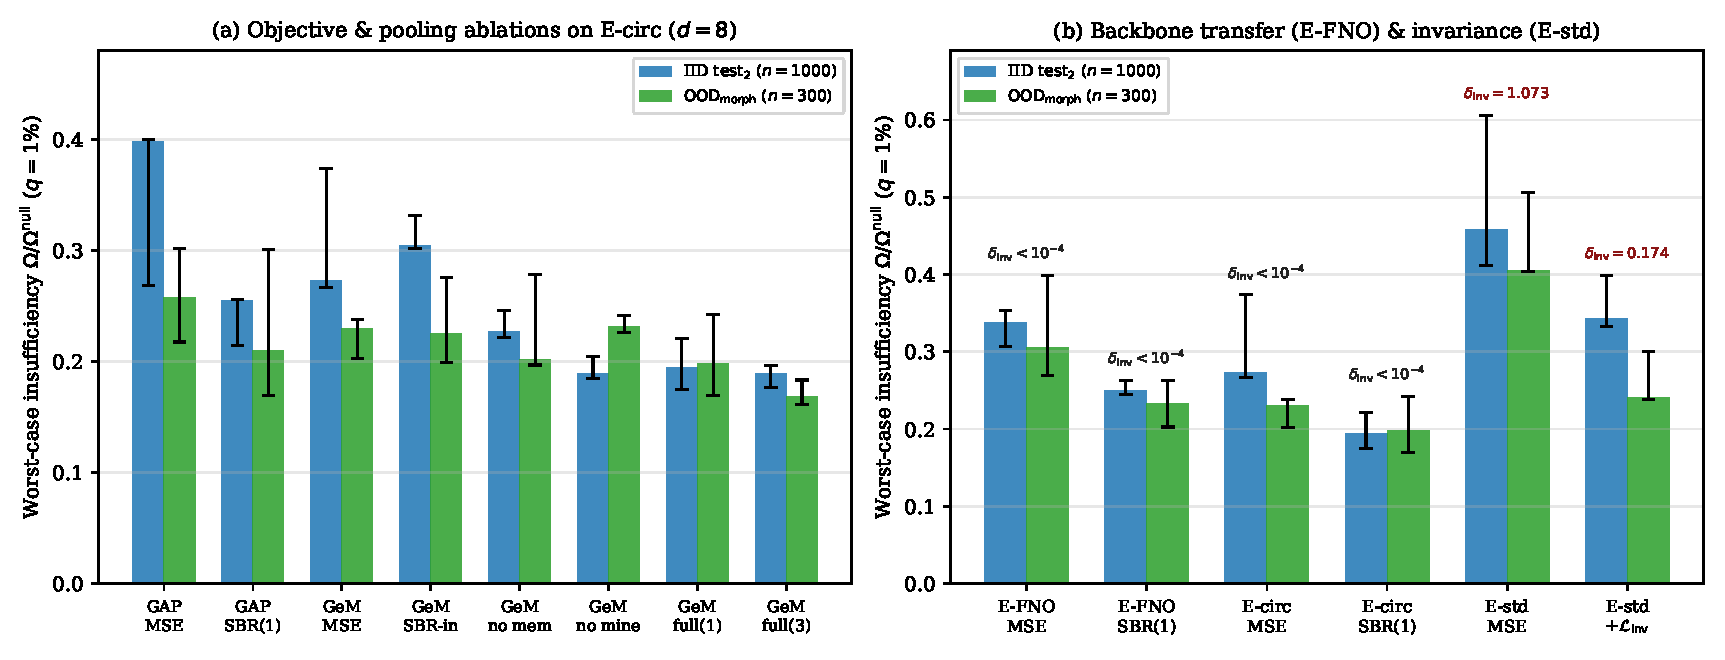
\includegraphics[width=0.98\textwidth]{fig_phase3_ablations.pdf}
\caption{Component ablations ($d=8$, 3-seed medians and min/max ranges on \texttt{test2} and \texttt{ood\_morphology}). Left: Exploratory objective and pooling decomposition. Right: Schedule-matched spectral \texttt{E-FNO} backbone transfer vs.\ symmetry breakdown in zero-padded \texttt{E-std}.}
\label{fig:phase3_ablations}
\end{figure}

Table~\ref{tab:ablations_phase3} supports three observations:
(i)~In the schedule-matched 45-epoch comparisons, \texttt{SBR-CF} transfers cleanly to the spectral \texttt{E-FNO} backbone, cutting $\Omega/\Omega^{\rm null}$ from $0.338$ to $0.250$ on \texttt{test2} and from $0.306$ to $0.233$ on OOD while raising $R^2_{\rm McShane}$ from $0.922$ to $0.959$;
(ii)~the 45-epoch zero-padded configuration \texttt{E-std (no sym) + GeM + MSE} exhibits a large invariance defect $\delta_{\rm inv}=1.073$ and $\Omega/\Omega^{\rm null}=0.459$ ($R^2_{\rm McShane}=0.805$); within the strictly schedule-matched 45-epoch pair, adding the soft invariance penalty $\mathcal L_{\rm inv}$ reduces $\delta_{\rm inv}$ from $1.073$ to $0.174$, lowers $\Omega/\Omega^{\rm null}$ from $0.459$ to $0.343$, and raises $R^2_{\rm McShane}$ from $0.805$ to $0.901$ (compared with $\Omega/\Omega^{\rm null}=0.338$, $R^2_{\rm McShane}=0.922$ for 45-epoch equivariant \texttt{E-FNO + GeM + MSE} and $\Omega/\Omega^{\rm null}=0.273$, $R^2_{\rm McShane}=0.947$ for 60-epoch \texttt{E-circ + GeM + MSE}); and
(iii)~in the exploratory 45-epoch objective-component runs, both \texttt{SBR-CF (no mem)} ($0.227$) and \texttt{SBR-CF (no mine)} ($0.189$) outperform 60-epoch \texttt{MSE} ($0.273$) and \texttt{SBR-in} ($0.303$) on IID \texttt{test2}, whereas on \texttt{ood\_morphology} \texttt{no mem} lowers $\Omega/\Omega^{\rm null}$ to $0.202$ while \texttt{no mine} gives $0.232$ (vs.\ $0.229$ for \texttt{MSE}, $0.228$ for \texttt{SBR-in}, and $0.199$ for full \texttt{SBR-CF} $\lambda_{\rm cf}=1$), suggesting that cross-batch memory primarily aids IID coverage while hard-query mining aids OOD coverage (subject to the 45- vs.\ 60-epoch schedule difference).

% ============================================================================
\section{Cross-Horizon, OOD-Physics, and Phase-Field Fracture Transfer (Experiments G--H)}
\label{sec:transfer_pf}

\subsection{Experiment G (Part 1): Cross-horizon transfer matrix across $R_E$ and $R_H(\beta)$}

Table~\ref{tab:transfer_i16} and Figure~\ref{fig:transfer_and_pf}(a) evaluate frozen-encoder transfer across $R_E$, $R_H(2)$, $R_H(20)$, and $R_H(40)$ on \texttt{test2} ($n=1{,}000$) under $d_{\rm white}$, refitting only the whitening transform and the McShane readout on each target. Encoders trained on bulk energy ($R_E$) or mild heterogeneity ($R_H(2)$) fail to resolve sharp stress-tail hazards ($\Omega/\Omega^{\rm null}=0.480\text{--}0.534$ on $R_H(20), R_H(40)$). Conversely, under $d_{\rm white}$ and McShane interpolation, \texttt{SBR-CF} trained solely on $R_H(20)$ transfers both forward to $R_H(40)$ ($\Omega/\Omega^{\rm null}=0.196\text{--}0.213$, outperforming \texttt{MSE} trained directly on $R_H(40)$ at $0.280$) and backward to $R_E$ ($0.110$, $R^2_{\rm McShane}=0.947$) and $R_H(2)$ ($0.209$, $R^2_{\rm McShane}=0.952$), whereas \texttt{RNC}'s 1D curve specialized to $R_H(20)$ degrades under whitened McShane transfer to $R_H(2)$ ($\Omega/\Omega^{\rm null}=0.469$, $R^2_{\rm McShane}=0.840$).

\begin{table}[ht!]
\centering
\caption{Experiment G (Part 1): Cross-horizon transfer matrix on \texttt{test2} ($n=1{,}000$, $d=8$, 3-seed medians of $\Omega/\Omega^{\rm null}$ and $R^2_{\rm McShane}$ under $d_{\rm white}$).}
\label{tab:transfer_i16}
\footnotesize
\setlength{\tabcolsep}{4.0pt}
\begin{tabular}{llcccccccc}
\toprule
Source Model & Source & \multicolumn{4}{c}{$\Omega/\Omega^{\rm null}$ ($\downarrow$) on $R_{\rm tgt}$} & \multicolumn{4}{c}{$R^2_{\rm McShane}$ ($\uparrow$) on $R_{\rm tgt}$} \\
\cmidrule(lr){3-6}\cmidrule(lr){7-10}
 & $R_{\rm src}$ & $R_E$ & $R_H(2)$ & $R_H(20)$ & $R_H(40)$ & $R_E$ & $R_H(2)$ & $R_H(20)$ & $R_H(40)$ \\
\midrule
\texttt{MSE (GAP)} & $R_E$ & \textbf{0.084} & 0.208 & 0.480 & 0.534 & \textbf{0.970} & 0.973 & 0.809 & 0.763 \\
\texttt{MSE (GeM)} & $R_H(2)$ & 0.129 & \textbf{0.188} & 0.510 & 0.531 & 0.941 & \textbf{0.976} & 0.768 & 0.714 \\
\texttt{MSE (GeM)} & $R_H(40)$ & 0.168 & 0.269 & 0.267 & 0.280 & 0.891 & 0.919 & 0.938 & 0.934 \\
\midrule
\texttt{MSE (GeM)} & $R_H(20)$ & 0.162 & 0.258 & 0.273 & 0.302 & 0.904 & 0.916 & 0.947 & 0.930 \\
\texttt{SBR-in} ($\lambda=1$) & $R_H(20)$ & 0.170 & 0.265 & 0.303 & 0.338 & 0.913 & 0.918 & 0.926 & 0.915 \\
\texttt{RankSim} ($\gamma=1$) & $R_H(20)$ & 0.165 & 0.307 & 0.261 & 0.286 & 0.870 & 0.902 & 0.924 & 0.900 \\
\texttt{RNC} ($\tau=1.0$) & $R_H(20)$ & 0.171 & 0.469 & 0.225 & 0.306 & 0.873 & 0.840 & 0.915 & 0.908 \\
\texttt{SBR-CF} ($\lambda=1$) & $R_H(20)$ & 0.120 & 0.249 & 0.192 & \textbf{0.196} & 0.909 & 0.937 & \textbf{0.962} & 0.954 \\
\texttt{SBR-CF} ($\lambda=3$) & $R_H(20)$ & \textbf{0.110} & \textbf{0.209} & \textbf{0.188} & 0.213 & \textbf{0.947} & \textbf{0.952} & 0.961 & \textbf{0.956} \\
\bottomrule
\end{tabular}
\end{table}

\subsection{Experiment G (Part 2): $90^\circ$ rotation check and OOD-physics transfer ($\kappa\in\{5,20\}$ and biaxial strain)}

Because the encoder takes only the binary microstructure image $x$ as input, changing the stiffness contrast $\kappa\in\{5,20\}$ or applying biaxial macroscopic strain $\bar\varepsilon=(1.0,0.5,0.0)$ changes the response $R(x)$ without changing $x$. We therefore pose OOD-physics transfer by freezing the $\kappa=10$, uniaxial $e_1$-trained encoder, evaluating $\Omega/\Omega^{\rm null}$ ($d_{\rm white}$) on the $n=300$ \texttt{test1} cells, and fitting linear ridge and McShane readouts on $n_{\rm few}\in\{50,200\}$ adaptation cells from \texttt{val}. Simultaneously, we verify $90^\circ$ load rotation ($\bar\varepsilon=e_2\otimes e_2$ at $\kappa=10$): continuum/FFT equivalence $R(x;e_2)=R(\operatorname{rot}_{90}(x);e_1)$ holds to $7.6\times 10^{-14}$, whereas feeding unrotated embeddings $E_\theta(x)$ to predict $R_H(x;e_2)$ collapses $R^2_{\rm ridge}$ to $\le 0.059$, confirming that $90^\circ$ rotation is not a symmetry of an anisotropic cell under fixed load.

\begin{table}[ht!]
\centering
\caption{Experiment G (Part 2): Zero-shot $90^\circ$ load-rotation check ($\bar\varepsilon=e_2\otimes e_2$) and few-shot OOD-physics transfer across contrast $\kappa\in\{5,20\}$ and biaxial strain $\bar\varepsilon=(1.0,0.5,0.0)$ on $R_H(\beta=20)$ ($n=300$ test cells, frozen $\kappa=10$ uniaxial encoders, $d=8$, 3-seed medians).}
\label{tab:ood_physics_rot}
\footnotesize
\setlength{\tabcolsep}{2.8pt}
\resizebox{\textwidth}{!}{%
\begin{tabular}{llcccccc}
\toprule
Regime & Metric / Adaptation & \texttt{MSE} & \texttt{SBR-in} & \texttt{RankSim} & \texttt{RNC} & \texttt{SBR-CF} & \texttt{SBR-CF} \\
 & & ($\lambda=0$) & ($\lambda=1$) & ($\gamma=1$) & ($\tau=1$) & ($\lambda=1$) & ($\lambda=3$) \\
\midrule
IID Ref.\ ($\kappa=10, e_1$)
 & $\Omega/\Omega^{\rm null}$ ($n=300$, $d_{\rm white}$) & 0.176 & 0.195 & 0.181 & 0.152 & \textbf{0.121} & 0.133 \\
 & Zero-shot $R^2_{\rm McShane}$ / $R^2_{\rm ridge}$ & 0.942 / 0.956 & 0.922 / 0.942 & 0.937 / 0.954 & 0.931 / \textbf{0.978} & \textbf{0.965} / 0.947 & 0.958 / 0.959 \\
\midrule
Rotation ($\kappa=10, e_2$)
 & $\Omega/\Omega^{\rm null}$ on $\operatorname{rot}_{90}(x)$ & 0.312 & 0.299 & 0.298 & 0.287 & 0.230 & \textbf{0.181} \\
 & Zero-shot $R^2_{\rm McShane}$ / $R^2_{\rm ridge}$ & 0.944 / 0.970 & 0.922 / 0.963 & 0.940 / 0.976 & 0.927 / \textbf{0.991} & 0.953 / 0.975 & \textbf{0.957} / 0.974 \\
 & Unrotated control $\Omega/\Omega^{\rm null}$ / $R^2_{\rm ridge}$ & 0.605 / 0.042 & 0.720 / 0.059 & 0.509 / 0.024 & 0.823 / $-0.010$ & 0.459 / 0.015 & 0.522 / 0.017 \\
\midrule
OOD-Phys: $\kappa=5$
 & $\Omega/\Omega^{\rm null}$ ($n=300$, $d_{\rm white}$) & 0.197 & 0.189 & 0.186 & 0.185 & \textbf{0.137} & 0.143 \\
 & Few-shot $n_{\rm few}=50$: $R^2_{\rm Mc}$ / $R^2_{\rm ridge}$ & 0.610 / 0.951 & 0.586 / 0.938 & 0.668 / 0.948 & 0.498 / \textbf{0.975} & 0.620 / 0.921 & \textbf{0.739} / 0.937 \\
 & Few-shot $n_{\rm few}=200$: $R^2_{\rm Mc}$ / $R^2_{\rm ridge}$ & 0.871 / 0.963 & 0.818 / 0.951 & 0.859 / 0.953 & 0.831 / \textbf{0.976} & \textbf{0.887} / 0.950 & 0.885 / 0.960 \\
\midrule
OOD-Phys: $\kappa=20$
 & $\Omega/\Omega^{\rm null}$ ($n=300$, $d_{\rm white}$) & 0.153 & 0.186 & 0.170 & 0.157 & \textbf{0.113} & 0.149 \\
 & Few-shot $n_{\rm few}=50$: $R^2_{\rm Mc}$ / $R^2_{\rm ridge}$ & 0.558 / 0.929 & 0.518 / 0.913 & 0.548 / 0.925 & 0.455 / \textbf{0.966} & 0.574 / 0.914 & \textbf{0.661} / 0.934 \\
 & Few-shot $n_{\rm few}=200$: $R^2_{\rm Mc}$ / $R^2_{\rm ridge}$ & 0.824 / 0.941 & 0.772 / 0.924 & 0.817 / 0.940 & 0.804 / \textbf{0.970} & \textbf{0.865} / 0.927 & 0.850 / 0.946 \\
\midrule
OOD-Phys: Biaxial
 & $\Omega/\Omega^{\rm null}$ ($n=300$, $d_{\rm white}$) & 0.166 & 0.159 & 0.190 & 0.254 & \textbf{0.118} & 0.168 \\
$\bar\varepsilon=(1, 0.5, 0)$
 & Few-shot $n_{\rm few}=50$: $R^2_{\rm Mc}$ / $R^2_{\rm ridge}$ & 0.557 / 0.915 & 0.531 / 0.897 & 0.582 / 0.908 & 0.507 / \textbf{0.948} & 0.590 / 0.890 & \textbf{0.695} / 0.904 \\
 & Few-shot $n_{\rm few}=200$: $R^2_{\rm Mc}$ / $R^2_{\rm ridge}$ & 0.825 / 0.926 & 0.793 / 0.908 & 0.808 / 0.912 & 0.778 / \textbf{0.943} & \textbf{0.861} / 0.904 & 0.847 / 0.926 \\
\bottomrule
\end{tabular}%
}
\end{table}

Table~\ref{tab:ood_physics_rot} highlights complementary strengths of \texttt{SBR-CF} and \texttt{RNC}:
(i)~\texttt{SBR-CF} achieves the lowest whitened worst-case insufficiency across all four shifted regimes ($0.181$ on $90^\circ$ rotation at $\lambda_{\rm cf}=3$; $0.137, 0.113, 0.118$ on $\kappa=5, \kappa=20$, and biaxial loading at $\lambda_{\rm cf}=1$) and the highest few-shot McShane interpolation $R^2_{\rm McShane}$ at both $n_{\rm few}=50$ ($0.739, 0.661, 0.695$) and $n_{\rm few}=200$ ($0.887, 0.865, 0.861$);
(ii)~simultaneously, \texttt{RNC} ($\tau=1.0$) achieves the highest linear ridge $R^2_{\rm ridge}$ across the contrast and biaxial shifts ($0.976$ on $\kappa=5$, $0.970$ on $\kappa=20$, and $0.943$ on biaxial strain at $n_{\rm few}=200$, vs.\ $0.950\text{--}0.960$, $0.927\text{--}0.946$, and $0.904\text{--}0.926$ for \texttt{SBR-CF}), because $R_H(20)$ under modified contrast or biaxial load remains strongly correlated with the uniaxial scalar ordering captured by \texttt{RNC}'s leading axis, even though whitening its 7 orthogonal directions inflates its biaxial $\Omega/\Omega^{\rm null}$ to $0.254$.

\subsection{Experiment H (Part 1): Seed-combined local-swap conditional permutation tests (\texttt{T1}--\texttt{T6}) and statistical power}
\label{sec:cond_tests}

To test whether pretrained embeddings carry incremental worst-case signal beyond explicit physics descriptors ($D_0=E_1$ or $D_0=E_1+J_{1.5\ell}$) on the $n=150$ multi-inclusion phase-field design cells, we apply the local-swap conditional permutation test \cite{Berrett2020,Kim2022}. Because taking the median of three seed-level $p$-values is a descriptive summary rather than a single combined $p$-value, we construct a seed-combined local-swap conditional permutation test: for each local swap $b\in\{1,\dots,B\}$ ($B=2{,}000$, $k_{\rm nn}=5$ in standardized $D_0$), all three seeds $s\in\{0,1,2\}$ are permuted synchronously by the same swap permutation $\pi_b$, and the seed-aggregated statistic
\begin{equation}
\bar\Omega(q) = \frac13\sum_{s=0}^2\Omega_s(q)
\qquad (q=1\%)
\label{eq:seed_combined_stat}
\end{equation}
is compared against its permutation distribution $\{\bar\Omega^{(b)}(q)\}_{b=1}^B$, with Holm step-down correction \cite{Holm1979} across all 6 tests \texttt{T1}--\texttt{T6}. While synchronous permutation across seeds accounts for cross-seed correlation without ad-hoc $p$-value medians, the conditional null calibration remains \emph{approximate} because swapping $k_{\rm nn}=5$ nearest neighbors in a continuous 6- or 7-dimensional descriptor space $D_0$ only approximates conditional exchangeability \cite{Kim2022}. Table~\ref{tab:cond_test_h6} reports the seed-combined ratio $\bar\Omega/\bar\Omega^{\rm cnull}$, the seed-combined $p_{\rm raw}$ ($p_{\rm Holm}$), and the number of individual seeds achieving $p_{\rm Holm}<0.05$ (individual seed $p$-values and ensemble-distance tests are reported in Appendix~\ref{app:cond_power}).

To calibrate empirical Type-I error and finite-sample detection power on \texttt{T5} ($R_\sigma\mid E_1+J_{1.5\ell}$), we generate synthetic responses from the linear-Gaussian conditional nuisance law
\begin{equation}
R_{\rm syn}^{(\eta,m)} = \widehat R_{\rm OLS}(D_0) + \eta\,\sigma_{R_\sigma}\,u_{\rm orth}(Z) + \varepsilon^{(m)},
\qquad
\varepsilon^{(m)}\stackrel{\rm iid}{\sim}\mathcal N(0,\hat\sigma_{\rm res}^2 I_{150}),
\label{eq:syn_cond_power}
\end{equation}
where $\widehat R_{\rm OLS}(D_0)$ is the linear regression fit of $R_\sigma$ on $D_0=E_1+J_{1.5\ell}$ ($\hat\sigma_{\rm res}$ is the empirical residual standard deviation) and $u_{\rm orth}(Z)\in\R^{150}$ is constructed in \path{scripts/run_phase5a_ml_and_stats_controls.py} by concatenating the column-standardized 8D embeddings of the three seeds of \texttt{SBR-CF} ($\lambda_{\rm cf}=1.0$) into a $150\times 24$ matrix $Z_{\rm concat}$, projecting $Z_{\rm concat}$ orthogonally onto the complement of $\Phi=[1,\operatorname{zscore}(D_0)]$, extracting the first left singular vector of $(I-\Phi\Phi^\dagger)Z_{\rm concat}$, and standardizing it to zero mean and unit variance. At $\eta=0$, $R_{\rm syn}^{(0,m)}\perp\!\!\!\perp Z\mid D_0$ holds by construction; across $\eta\in\{0, 0.10, 0.15, 0.20, 0.25, 0.35, 0.50\}$, we evaluate $150$ Monte Carlo replicates per $\eta$ (Table~\ref{tab:cond_power_t5} in Appendix~\ref{app:cond_power}). Because this Monte Carlo study simulates the single test \texttt{T5} in isolation rather than all 6 tests \texttt{T1}--\texttt{T6} jointly, Table~\ref{tab:cond_power_t5} reports unadjusted rejection rates at $\alpha\in\{0.05,0.10\}$ together with the single-test Bonferroni threshold $\alpha/6=0.05/6\approx 0.0083$ (the strictest first-step threshold of a 6-test Holm procedure).

\begin{table}[ht!]
\centering
\caption{Experiment H (Part 1): Seed-combined local-swap conditional permutation tests (\texttt{T1}--\texttt{T6}, Eq.~\eqref{eq:seed_combined_stat}, $B=2{,}000$, $q=1\%$, $k_{\rm nn}=5$ in standardized $D_0$) across the $n=150$ multi-inclusion phase-field design cells. Columns report $\bar\Omega/\bar\Omega^{\rm cnull}$, seed-combined Holm-adjusted $p_{\rm Holm}$ (across the 6-test family \texttt{T1}--\texttt{T6}), and count of individual seeds with $p_{\rm Holm}<0.05$ ($S_{\rm sig}/3$). Bold denotes $p_{\rm Holm}<0.05$.}
\label{tab:cond_test_h6}
\footnotesize
\setlength{\tabcolsep}{2.4pt}
\resizebox{\textwidth}{!}{%
\begin{tabular}{lllcccccccccc}
\toprule
Test & Target & Cond.\ $D_0$ & \multicolumn{2}{c}{\texttt{MSE} ($R_H(20)$)} & \multicolumn{2}{c}{\texttt{Tail-MSE} ($\lambda=3$)} & \multicolumn{2}{c}{\texttt{RankSim} ($\gamma=1$)} & \multicolumn{2}{c}{\texttt{RNC} ($\tau=1$)} & \multicolumn{2}{c}{\texttt{SBR-CF} ($\lambda=1$ / $\lambda=3$)} \\
\cmidrule(lr){4-5}\cmidrule(lr){6-7}\cmidrule(lr){8-9}\cmidrule(lr){10-11}\cmidrule(lr){12-13}
 & & & Ratio & $p_{\rm Holm}$ ($S$) & Ratio & $p_{\rm Holm}$ ($S$) & Ratio & $p_{\rm Holm}$ ($S$) & Ratio & $p_{\rm Holm}$ ($S$) & Ratio ($\lambda=1,3$) & $p_{\rm Holm}$ ($\lambda=1,3$) \\
\midrule
\texttt{T1} & $R_E$ & $E_1$ (neg.\ ctrl) & 1.037 & 0.509 (0/3) & 0.848 & 0.314 (0/3) & 0.778 & 0.217 (0/3) & 1.062 & 1.000 (0/3) & 0.895 / 0.644 & 0.523 / \textbf{0.014} (0/3) \\
\texttt{T2} & $R_H(20)$ & $E_1$ & 0.754 & 0.110 (1/3) & \textbf{0.563} & \textbf{0.003} (2/3) & \textbf{0.537} & \textbf{0.012} (1/3) & \textbf{0.184} & \textbf{0.005} (3/3) & \textbf{0.501} / \textbf{0.387} & \textbf{0.003} / \textbf{0.005} (2,3/3) \\
\texttt{T3} & $R_H(20)$ & $E_1+J_{1.5\ell}$ & \textbf{0.640} & \textbf{0.009} (2/3) & \textbf{0.609} & \textbf{0.003} (2/3) & \textbf{0.637} & \textbf{0.020} (1/3) & \textbf{0.229} & \textbf{0.003} (3/3) & \textbf{0.550} / \textbf{0.448} & \textbf{0.003} / \textbf{0.003} (2,3/3) \\
\texttt{T4} & $R_\sigma$ & $E_1$ & 0.707 & 0.110 (0/3) & \textbf{0.657} & \textbf{0.022} (0/3) & \textbf{0.612} & \textbf{0.012} (1/3) & 0.627 & 0.376 (0/3) & 0.726 / 0.668 & 0.262 / 0.139 (0/3) \\
\texttt{T5} & $R_\sigma$ & $E_1+J_{1.5\ell}$ & 0.893 & 0.411 (0/3) & \textbf{0.762} & \textbf{0.043} (1/3) & 0.873 & 0.228 (0/3) & 0.957 & 1.000 (0/3) & 0.876 / 0.945 & 0.271 / 0.307 (1,0/3) \\
\texttt{T6} & $R_{\rm path}$ & $E_1+J_{1.5\ell}$ & 0.837 & 0.411 (1/3) & 0.931 & 0.314 (0/3) & 0.809 & 0.228 (0/3) & 1.119 & 1.000 (0/3) & 0.899 / 0.669 & 0.539 / 0.164 (0/3) \\
\bottomrule
\end{tabular}%
}
\end{table}

Table~\ref{tab:cond_test_h6} and the power calibration in Appendix~\ref{app:cond_power} (Tables~\ref{tab:cond_seed_detail}--\ref{tab:cond_power_t5}) establish three precise statistical conclusions:
\begin{enumerate}
    \item \textbf{Low finite-sample detection power at $n=150$ and non-exclusion of large effects:} Under the synthetic conditional null ($\eta=0$, where $\eta$ in Eq.~\eqref{eq:syn_cond_power} is the dimensionless signal amplitude in $\sigma_{R_\sigma}$ units), the local-swap test on \texttt{T5} has empirical rejection rate $0.020$ at nominal $\alpha=0.05$ ($0.060$ at $\alpha=0.10$, and $0.000$ at the Bonferroni threshold $\alpha=0.05/6$). However, because the $q=1\%$ tail on $n=150$ cells contains only $\binom{150}{2}\times 0.01\approx 112$ pairs, statistical power is low even for substantial conditional signals: at $\eta=0.35$ (signal amplitude $0.35\sigma_{R_\sigma}$, explaining $11.0\%$ of total variance and $71.3\%$ of residual variance), unadjusted $\alpha=0.05$ power is $7.3\%$ ($0.7\%$ at $\alpha=0.05/6$), and at $\eta=0.50$ (signal amplitude $0.50\sigma_{R_\sigma}$, explaining $20.1\%$ of total variance and $83.5\%$ of residual variance), unadjusted $\alpha=0.05$ power is only $\mathbf{28.0\%}$ ($51.3\%$ at $\alpha=0.10$, and $\mathbf{2.7\%}$ at the Bonferroni threshold $\alpha=0.05/6$). Thus, at $\eta=0.50$, $72\%$ of replicates fail to detect the signal at unadjusted $\alpha=0.05$ ($97.3\%$ at $\alpha=0.05/6$). Consequently, \emph{non-significant results on \texttt{T5} or \texttt{T6} cannot be used to rule out even large local conditional effects}, and the \texttt{T5} calibration does not calibrate \texttt{T6} ($R_{\rm path}\mid E_1+J_{1.5\ell}$, where $D_0$ explains almost no variance).
    \item \textbf{Approximate conditional exchangeability in 6D/7D $D_0$ and negative-control behavior (\texttt{T1}):} Local-swap permutations over $k_{\rm nn}=5$ nearest neighbors in a 6- or 7-dimensional continuous descriptor space $D_0$ provide only \emph{approximate} conditional exchangeability \cite{Kim2022}: when the true response varies across $k_{\rm nn}=5$ neighbors in $D_0$ and the learned embedding $Z$ correlates with within-neighborhood variations of $D_0$, swapping neighbors can introduce a finite-sample local conditioning bias. Such finite-sample conditioning bias is a plausible explanation for the isolated seed-combined rejection on the negative control \texttt{T1} for \texttt{SBR-CF} ($\lambda_{\rm cf}=3$, $\bar\Omega/\bar\Omega^{\rm cnull}=0.644$, $p_{\rm Holm}=0.014$, although $0/3$ individual seeds reject at $p_{\rm Holm}<0.05$ and the ensemble-distance test gives $p_{\rm Holm}^{\rm ens}=0.183$; Table~\ref{tab:cond_seed_detail}), though a single test realization cannot isolate its cause. This approximate-exchangeability caveat applies symmetrically to both positive rejections and non-rejections across \texttt{T1}--\texttt{T6}.
    \item \textbf{Positive conditional detections (\texttt{T2}--\texttt{T5}):} Subject to the approximate exchangeability of $k_{\rm nn}=5$ local swaps, on $R_H(20)$, \texttt{SBR-CF} ($\lambda_{\rm cf}=1,3$), \texttt{Tail-MSE} ($\lambda_{\rm tail}=3$), \texttt{RankSim}, and \texttt{RNC} all reject the conditional null beyond both $E_1$ (\texttt{T2}: $p_{\rm Holm}=0.003\text{--}0.012$) and $E_1+J_{1.5\ell}$ (\texttt{T3}: $p_{\rm Holm}=0.003\text{--}0.020$). On peak fracture strength $R_\sigma$, \texttt{Tail-MSE} ($\lambda_{\rm tail}=3$) and \texttt{RankSim} ($\gamma=1$) reject \texttt{T4} ($R_\sigma\mid E_1$, $p_{\rm Holm}=0.022$ and $0.012$), and \texttt{Tail-MSE} ($\lambda_{\rm tail}=3$) also reaches nominal significance on \texttt{T5} ($R_\sigma\mid E_1+J_{1.5\ell}$, $\bar\Omega/\bar\Omega^{\rm cnull}=0.762$, $p_{\rm Holm}=0.043$, $1/3$ individual seeds; Table~\ref{tab:cond_seed_detail}), whereas \texttt{MSE}, \texttt{SBR-CF} ($\lambda_{\rm cf}=1,3$), \texttt{RankSim}, and \texttt{RNC} do not reject \texttt{T5} ($p_{\rm Holm}=0.228\text{--}1.000$) or \texttt{T6} ($p_{\rm Holm}=0.164\text{--}1.000$).
\end{enumerate}

\subsection{Experiment H (Part 2): Frozen AT1 phase-field fracture transfer, extreme stress errors, and strip-shift barrier $b_S$}
\label{sec:pf_transfer_results}

We fit linear ridge readouts by 5-fold cell-grouped cross-validation on the $n=180$ non-laminate design cells and evaluate frozen out-of-sample predictions across \texttt{Set B} ($n=45$), \texttt{Set O} ($\alpha=6$, $n=12$), \texttt{Set C1} ($n=30$), and \texttt{Set C2} ($n_{\rm inc}\in\{16,25\}$, $n=12$). For clarity, we separate the evaluation into two tables: Table~\ref{tab:pf_transfer_r2} reports out-of-sample $R^2$ across all five fracture splits for $R_\sigma$ and $R_{\rm path}$, while Table~\ref{tab:pf_transfer_extremes} reports detailed tail and physical stress error metrics---RMSE, 90th-percentile error $P_{90}|\Delta R_\sigma|$, maximum absolute error $\max|\Delta R_\sigma|$, and mean and maximum relative error in physical peak stress
\begin{equation}
\delta_{\sigma,\rm rel} = \left|\frac{\widehat\sigma_{\rm peak}-\sigma_{\rm peak}}{\sigma_{\rm peak}}\right| = \big|\exp(\widehat R_\sigma - R_\sigma) - 1\big|\times 100\%
\end{equation}
---on Design CV ($n=180$), blind Set~B ($n=45$), and prospective Set~C2 ($n=12$).

\begin{table}[ht!]
\centering
\caption{Experiment H (Part 2a): Out-of-sample $R^2$ ($\uparrow$, 3-seed medians) on frozen AT1 phase-field fracture splits across Design CV ($n=180$), blind Set~B ($n=45$ for $R_\sigma$, $n_{\rm eff}=44$ for $R_{\rm path}$), high-aspect-ratio Set~O ($\alpha=6$, $n=12$ for $R_\sigma$, $n_{\rm eff}=11$ for $R_{\rm path}$), prospective Set~C1 ($n=30$), and high-inclusion-count prospective Set~C2 ($n=12$). Bold entries mark the best model within each group (physics-only, standalone image-only, and hybrid solved-field + embedding).}
\label{tab:pf_transfer_r2}
\footnotesize
\setlength{\tabcolsep}{3.6pt}
\resizebox{\textwidth}{!}{%
\begin{tabular}{llcccccc}
\toprule
Target & Representation & FFT Solve at Test? & Design CV$_{180}$ & Blind Set B & OOD Set O & Prosp.\ Set C1 & Prosp.\ Set C2 \\
\midrule
$R_\sigma$
 & \texttt{E1} (mean strains + gaps) & Yes (FFT) & 0.319 & 0.298 & $-1.365$ & 0.536 & $-3.424$ \\
 & \texttt{E1 + RH\_b20} (scalar hazard) & Yes (FFT) & 0.511 & 0.454 & 0.538 & 0.707 & $-1.407$ \\
 & \texttt{E1 + J\_1.5} (critical distance)$^\dagger$ & Yes (FFT) & \textbf{0.881} & \textbf{0.930} & \textbf{0.945} & \textbf{0.906} & \textbf{0.679} \\
\cmidrule(lr){2-8}
 & \texttt{MSE} ($R_H(20)$) alone & \textbf{No (Img)} & 0.562 & 0.593 & \textbf{0.884} & 0.744 & 0.048 \\
 & \texttt{Tail-MSE} ($\lambda=1$) alone & \textbf{No (Img)} & \textbf{0.661} & 0.606 & 0.784 & 0.766 & \textbf{0.398} \\
 & \texttt{Tail-MSE} ($\lambda=3$) alone & \textbf{No (Img)} & 0.637 & 0.615 & 0.828 & 0.757 & 0.360 \\
 & \texttt{RankSim} ($\gamma=1$) alone & \textbf{No (Img)} & 0.604 & 0.563 & 0.864 & 0.789 & 0.019 \\
 & \texttt{RNC} ($\tau=1$) alone & \textbf{No (Img)} & 0.557 & 0.543 & 0.685 & 0.751 & $-1.342$ \\
 & \texttt{SBR-CF} ($\lambda_{\rm cf}=1$) alone & \textbf{No (Img)} & 0.551 & 0.604 & 0.714 & 0.735 & 0.369 \\
 & \texttt{SBR-CF} ($\lambda_{\rm cf}=3$) alone & \textbf{No (Img)} & 0.592 & \textbf{0.628} & 0.790 & \textbf{0.812} & 0.111 \\
\cmidrule(lr){2-8}
 & \texttt{E1 + J\_1.5 + MSE} ($R_H(20)$) & Yes (FFT) & 0.954 & \textbf{0.968} & 0.976 & 0.964 & 0.922 \\
 & \texttt{E1 + J\_1.5 + Tail-MSE} ($\lambda=1$) & Yes (FFT) & 0.942 & 0.965 & 0.958 & 0.966 & 0.886 \\
 & \texttt{E1 + J\_1.5 + Tail-MSE} ($\lambda=3$) & Yes (FFT) & 0.960 & 0.964 & 0.973 & \textbf{0.973} & 0.905 \\
 & \texttt{E1 + J\_1.5 + RankSim} ($\gamma=1$) & Yes (FFT) & 0.946 & 0.967 & 0.970 & 0.964 & 0.901 \\
 & \texttt{E1 + J\_1.5 + RNC} ($\tau=1$) & Yes (FFT) & 0.883 & 0.948 & 0.945 & 0.920 & 0.766 \\
 & \texttt{E1 + J\_1.5 + SBR-CF} ($\lambda=1$) & Yes (FFT) & \textbf{0.963} & 0.964 & 0.973 & 0.967 & \textbf{0.939} \\
 & \texttt{E1 + J\_1.5 + SBR-CF} ($\lambda=3$) & Yes (FFT) & 0.955 & 0.967 & \textbf{0.982} & 0.971 & 0.918 \\
\midrule
$R_{\rm path}^{\ddagger}$
 & \texttt{E1 + J\_1.5} & Yes (FFT) & $-0.078$ & 0.046 & $-2.658$ & --- & --- \\
 & \texttt{E1 + J\_1.5 + SBR-CF} ($\lambda=1$) & Yes (FFT) & 0.105 & \textbf{0.112} & $-0.915$ & --- & --- \\
 & \texttt{E1 + J\_1.5 + SBR-CF} ($\lambda=3$) & Yes (FFT) & \textbf{0.120} & 0.062 & $-1.355$ & --- & --- \\
\bottomrule
\end{tabular}%
}
\par\smallskip\raggedright{\footnotesize $^\dagger$Under unregularized OLS \cite{GomezOvalle2026}, \texttt{E1+J\_1.5} attains $R^2=0.879$ (CV), $0.932$ (Set~B), $0.941$ (Set~O), $0.905$ (Set~C1), and $0.689$ (Set~C2); under the common 5-fold CV ridge grid $\alpha\in\{10^{-3},\dots,20\}$ used for all rows above, \texttt{E1+J\_1.5} attains $0.881, 0.930, 0.945, 0.906, 0.679$.\\
$^\ddagger$For $R_{\rm path}$ (Eq.~\eqref{eq:cpath_def}), all rows use the identical valid-cell mask with effective sample sizes $n_{\rm eff}=180$ (Design CV), $n_{\rm eff}=44$ (Set~B, excluding non-percolating en-echelon cell $\texttt{bid}=72$), and $n_{\rm eff}=11$ (Set~O, excluding $\texttt{bid}=106$); see Section~\ref{sec:pf} and \path{data/frozen/blind_pf.csv}.}
\end{table}

\begin{table}[ht!]
\centering
\caption{Experiment H (Part 2b): Detailed tail and physical peak-stress error metrics ($\downarrow$, 3-seed medians) on Design CV ($n=180$), blind Set~B ($n=45$), and high-inclusion-count prospective Set~C2 ($n=12$). Columns report RMSE, $P_{90}|\Delta R_\sigma|$, $\max|\Delta R_\sigma|$, and mean/maximum relative peak-stress error $\delta_{\sigma,\rm rel}$ ($\%$).}
\label{tab:pf_transfer_extremes}
\footnotesize
\setlength{\tabcolsep}{3.0pt}
\resizebox{\textwidth}{!}{%
\begin{tabular}{lccccccccc}
\toprule
Representation ($R_\sigma$) & \multicolumn{2}{c}{Design CV ($n=180$)} & \multicolumn{2}{c}{Blind Set B ($n=45$)} & \multicolumn{5}{c}{Prospective Set C2 ($n=12$, $n_{\rm inc}\in\{16,25\}$)} \\
\cmidrule(lr){2-3}\cmidrule(lr){4-5}\cmidrule(lr){6-10}
 & Mean $\delta_{\sigma,\rm rel}$ & Max $\delta_{\sigma,\rm rel}$ & Mean $\delta_{\sigma,\rm rel}$ & Max $\delta_{\sigma,\rm rel}$ & RMSE & $P_{90}|\Delta R_\sigma|$ & $\max|\Delta R_\sigma|$ & Mean $\delta_{\sigma,\rm rel}$ & Max $\delta_{\sigma,\rm rel}$ \\
\midrule
\texttt{E1} (mean strains + gaps) & 7.12\% & 23.24\% & 8.05\% & 21.06\% & 0.0989 & 0.1337 & 0.1356 & 8.95\% & 12.68\% \\
\texttt{E1 + RH\_b20} (scalar hazard) & 6.08\% & 15.47\% & 7.21\% & 16.75\% & 0.0729 & 0.0961 & 0.1158 & 6.43\% & 10.94\% \\
\texttt{E1 + J\_1.5} (critical distance) & \textbf{2.84\%} & \textbf{7.61\%} & \textbf{2.26\%} & \textbf{4.53\%} & \textbf{0.0266} & \textbf{0.0396} & \textbf{0.0417} & \textbf{2.35\%} & \textbf{4.09\%} \\
\midrule
\texttt{MSE} ($R_H(20)$) alone & 5.58\% & 15.09\% & 6.01\% & 14.73\% & 0.0459 & 0.0700 & 0.0921 & 3.69\% & 8.80\% \\
\texttt{Tail-MSE} ($\lambda=1$) alone & \textbf{4.93\%} & \textbf{13.26\%} & 5.91\% & 15.35\% & \textbf{0.0365} & 0.0619 & 0.0753 & \textbf{2.72\%} & 7.82\% \\
\texttt{Tail-MSE} ($\lambda=3$) alone & 5.10\% & 16.68\% & 5.83\% & 15.67\% & 0.0376 & \textbf{0.0575} & \textbf{0.0731} & 3.21\% & \textbf{7.04\%} \\
\texttt{RankSim} ($\gamma=1$) alone & 5.31\% & 18.20\% & 6.23\% & 13.54\% & 0.0466 & 0.0737 & 0.0899 & 3.60\% & 8.59\% \\
\texttt{RNC} ($\tau=1$) alone & 5.65\% & 19.56\% & 6.38\% & \textbf{13.23\%} & 0.0719 & 0.0953 & 0.1225 & 5.91\% & 11.53\% \\
\texttt{SBR-CF} ($\lambda_{\rm cf}=1$) alone & 5.64\% & 16.86\% & 5.92\% & 17.04\% & 0.0373 & 0.0632 & 0.0792 & 2.97\% & 7.61\% \\
\texttt{SBR-CF} ($\lambda_{\rm cf}=3$) alone & 5.39\% & 20.95\% & \textbf{5.73\%} & 13.77\% & 0.0443 & 0.0759 & 0.1004 & 3.44\% & 9.55\% \\
\midrule
\texttt{E1 + J\_1.5 + MSE} ($R_H(20)$) & 1.75\% & 5.17\% & \textbf{1.53\%} & 3.90\% & 0.0131 & 0.0193 & 0.0230 & 1.10\% & 2.27\% \\
\texttt{E1 + J\_1.5 + Tail-MSE} ($\lambda=1$) & 1.98\% & 5.32\% & 1.59\% & 4.14\% & 0.0159 & 0.0221 & 0.0338 & 1.20\% & 3.32\% \\
\texttt{E1 + J\_1.5 + Tail-MSE} ($\lambda=3$) & 1.64\% & \textbf{4.79\%} & 1.62\% & 4.25\% & 0.0145 & 0.0211 & 0.0287 & 1.14\% & 2.91\% \\
\texttt{E1 + J\_1.5 + RankSim} ($\gamma=1$) & 1.90\% & 4.93\% & 1.55\% & 3.35\% & 0.0148 & 0.0219 & 0.0245 & 1.26\% & 2.42\% \\
\texttt{E1 + J\_1.5 + RNC} ($\tau=1$) & 2.81\% & 7.92\% & 1.95\% & 4.52\% & 0.0228 & 0.0315 & 0.0435 & 1.88\% & 4.26\% \\
\texttt{E1 + J\_1.5 + SBR-CF} ($\lambda=1$) & \textbf{1.58\%} & 5.44\% & 1.62\% & 3.57\% & \textbf{0.0116} & \textbf{0.0191} & 0.0250 & \textbf{0.94\%} & 2.47\% \\
\texttt{E1 + J\_1.5 + SBR-CF} ($\lambda=3$) & 1.74\% & 5.26\% & 1.55\% & \textbf{3.23\%} & 0.0135 & 0.0206 & \textbf{0.0225} & 1.13\% & \textbf{2.26\%} \\
\bottomrule
\end{tabular}%
}
\par\smallskip\raggedright{\footnotesize Note: On Set~C2, Seed~2 of \texttt{E1+J\_1.5+SBR-CF ($\lambda=1$)} reaches $R^2=0.940$, $\max|\Delta R_\sigma|=0.0197$, and $\max\delta_{\sigma,\rm rel}=1.95\%$.}
\end{table}

\begin{figure}[ht!]
\centering
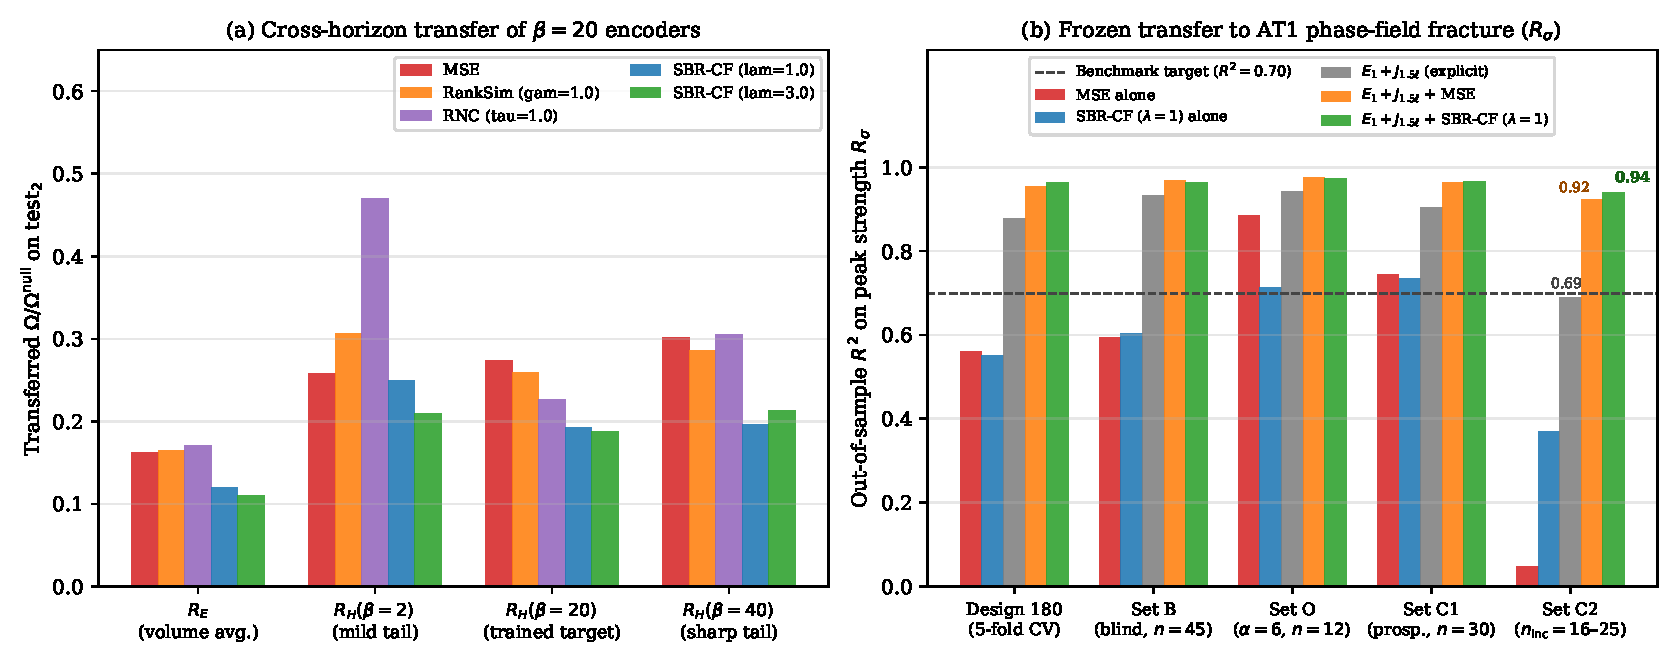
\includegraphics[width=0.98\textwidth]{fig_transfer_and_pf.pdf}
\caption{Left: Cross-horizon transfer matrix ($\Omega/\Omega^{\rm null}$ on \texttt{test2}). Right: Out-of-sample $R^2$ on peak fracture strength $R_\sigma$ across Design CV ($n=180$) and frozen Sets B, O, C1, C2, comparing $E_1+J_{1.5\ell}$ alone ($0.68\text{--}0.69$ on Set~C2) against $E_1+J_{1.5\ell}+\texttt{MSE}$ ($0.92$) and $E_1+J_{1.5\ell}+\texttt{SBR-CF}$ ($\lambda_{\rm cf}=1$, $0.94$).}
\label{fig:transfer_and_pf}
\end{figure}

\paragraph{Cell-block bootstrap uncertainty and balanced comparison across fracture models.}
Because predictions from the 3 random seeds on the same microstructure are correlated, all paired uncertainty intervals in Experiment~H are computed via a \emph{cell-level block bootstrap} ($B=2{,}000$ resamples of the $n_s$ physical cells with replacement, averaging the paired squared-error difference across the 3 seeds within each cell so that the effective sample size is $n_s=12$ on \texttt{Set C2} and $n_s=180$ on \texttt{Design CV}). Tables~\ref{tab:pf_transfer_r2}--\ref{tab:pf_transfer_extremes} support three nuanced conclusions:
\begin{enumerate}
    \item \textbf{Substantial gain of hybrid embeddings over $E_1+J_{1.5\ell}$ alone on Set~C2:} Augmenting $E_1+J_{1.5\ell}$ ($R^2=0.679\text{--}0.689$, mean/max $\delta_{\sigma,\rm rel}=2.35\%/4.09\%$) with any multi-dimensional $R_H(20)$ embedding (\texttt{MSE}, \texttt{Tail-MSE}, \texttt{RankSim}, or \texttt{SBR-CF}) lifts prospective \texttt{Set C2} $R^2$ to $0.886\text{--}0.939$ and cuts mean relative peak-stress error to $0.94\%\text{--}1.26\%$. For $E_1+J_{1.5\ell}+\texttt{SBR-CF}$ ($\lambda_{\rm cf}=1$) vs.\ $E_1+J_{1.5\ell}$ alone, the cell-block paired MSE reduction is $\Delta\text{MSE}=-6.10\times 10^{-4}$ on \texttt{Set C2} ($90\%$ cell-block bootstrap CI $[-9.04\times 10^{-4},\,-3.28\times 10^{-4}]$) and $\Delta\text{MSE}=-5.57\times 10^{-4}$ on \texttt{Design CV} ($90\%$ CI $[-6.56\times 10^{-4},\,-4.63\times 10^{-4}]$).
    \item \textbf{Comparison between $+$\texttt{SBR-CF} and $+$\texttt{MSE} on Set~C2:} Relative to the strong hybrid baseline $E_1+J_{1.5\ell}+\texttt{MSE}$ ($R^2=0.922$, RMSE $0.0131$, $P_{90}=0.0193$, mean $\delta_{\sigma,\rm rel}=1.10\%$), $E_1+J_{1.5\ell}+\texttt{SBR-CF}$ ($\lambda_{\rm cf}=1$) improves average and 90th-percentile accuracy ($R^2=\mathbf{0.939}$, RMSE $\mathbf{0.0116}$, $P_{90}=\mathbf{0.0191}$, mean $\delta_{\sigma,\rm rel}=\mathbf{0.94\%}$), with a modest, borderline cell-block paired MSE difference on the $n_s=12$ cells of $\Delta\text{MSE}=-5.26\times 10^{-5}$ ($90\%$ cell-block bootstrap CI $[-1.09\times 10^{-4},\,-1.59\times 10^{-6}]$). At the same time, the 3-seed median worst-case error on \texttt{Set C2} is slightly lower for $+$\texttt{SBR-CF} ($\lambda_{\rm cf}=3$, $\max\delta_{\sigma,\rm rel}=\mathbf{2.26\%}$) and $+$\texttt{MSE} ($2.27\%$) than for $+$\texttt{SBR-CF} ($\lambda_{\rm cf}=1$, $2.47\%$).
    \item \textbf{Standalone image-only transfer (no FFT solve at test time):} When predicting $R_\sigma$ directly from the binary image without an elastic solve at test time, \texttt{Tail-MSE} ($\lambda_{\rm tail}=1,3$) achieves the strongest standalone generalization on \texttt{Design CV} ($R^2=\mathbf{0.661}$) and \texttt{Set C2} ($R^2=\mathbf{0.398}$, mean $\delta_{\sigma,\rm rel}=\mathbf{2.72\%}$, max $\delta_{\sigma,\rm rel}=\mathbf{7.04\%}$ at $\lambda_{\rm tail}=3$), closely followed by standalone \texttt{SBR-CF} ($\lambda_{\rm cf}=1$, $R^2=0.369$, mean/max $\delta_{\sigma,\rm rel}=2.97\%/7.61\%$), both outperforming standalone \texttt{MSE} ($R^2=0.048$, $\Delta\text{MSE}=-3.21\times 10^{-4}$ for \texttt{SBR-CF} $\lambda_{\rm cf}=1$ vs.\ \texttt{MSE}) and \texttt{RNC} ($R^2=-1.342$).
\end{enumerate}

\paragraph{Direct measurement of the AT1 strip-translation barrier $b_S(x)\le b_{G_{x_1}}(x)$.}
Finally, to test whether the periodic translation invariance built into \texttt{E-circ} conflicts with the $2\%$ weakened vertical localization strip at $x_1=0.95$ in the AT1 phase-field solver (Section~\ref{sec:pf}), we evaluated 8 representative design cells (3 laminates, 3 multi-disk cells, and 2 multi-ellipse cells) across the 4-shift grid subset $S_{\rm grid}=\{0, 32, 64, 95\}$ pixels and the up-to-5-shift subset $S_{\rm all}=S_{\rm grid}\cup\{\Delta x_1^{\rm adv}\}$ that includes the cell-specific adversarial shift $\Delta x_1^{\rm adv}$ aligning each cell's maximum elastic driving hotspot $\arg\max_x(\psi_+/\psi_c)$ directly with the weakened strip $x_1=0.95$ (pixel $120$). Because $\Delta x_1^{\rm adv}=0\in S_{\rm grid}$ for laminate cells $16$ and $28$ ($|S_{\rm all}|=4$) while $\Delta x_1^{\rm adv}\notin S_{\rm grid}$ for the remaining 6 cells ($|S_{\rm all}|=5$), this design comprises $38$ distinct shifted cell configurations in total: the $8$ unshifted $\Delta x_1=0$ solutions from \texttt{design\_cells.csv} plus $30$ newly solved $\Delta x_1\ne 0$ AT1 trajectories (\path{results/pf_shifts/}), all computed with the identical \texttt{PhaseFieldRVE.run} protocol ($\delta_\varepsilon=\texttt{dE\_rel}=0.01$, Eq.~\eqref{eq:at1_stepping}) and all achieving complete post-peak separation ($\texttt{separated}=\texttt{True}$). Table~\ref{tab:strip_shifts} reports the empirical shift barriers $b_{S_{\rm grid}}(x)$ and $b_{S_{\rm all}}(x)$ (Eq.~\eqref{eq:b_shift}), together with both the minimax constant-prediction relative stress error $\tanh(b_S)\approx b_S$ and the full peak-to-trough relative peak-stress spread $(\sigma_{\max}-\sigma_{\min})/\sigma_{\min}=\exp(2b_S)-1$.

\begin{table}[ht!]
\centering
\caption{Direct AT1 phase-field evaluation of the finite-subset horizontal translation barrier $b_S(x)=\frac12[\max_{T\in S} R(Tx)-\min_{T\in S} R(Tx)]\le b_{G_{x_1}}(x)$ (Eq.~\eqref{eq:b_shift}) across 8 representative cells ($38$ distinct configurations: $8$ base $\Delta x_1=0$ solutions plus $30$ shifted trajectories, all solved with $\delta_\varepsilon=0.01$) under grid shifts $S_{\rm grid}=\{0,32,64,95\}$\,px ($b_{\rm shift}^{\rm grid}$) and $S_{\rm all}=S_{\rm grid}\cup\{\Delta x_1^{\rm adv}\}$ ($b_{\rm shift}^{\rm all}$, up to 5 shifts per cell). Columns report $b_{\rm shift}^{\rm grid}(R_\sigma)$, $b_{\rm shift}^{\rm all}(R_\sigma)$, the minimax relative peak-stress error ($\approx b_{\rm shift}^{\rm all}$) and full peak-to-trough relative spread ($\exp(2b_{\rm shift}^{\rm all})-1$), and $b_{\rm shift}^{\rm all}(R_{\rm path})$.}
\label{tab:strip_shifts}
\footnotesize
\setlength{\tabcolsep}{3.2pt}
\resizebox{\textwidth}{!}{%
\begin{tabular}{rlccccccc}
\toprule
Cell ID & Family ($n_{\rm inc}$, $f$) & $\Delta x_1^{\rm adv}$ & $\bar R_\sigma$ & $b_{\rm shift}^{\rm grid}(R_\sigma)$ & $b_{\rm shift}^{\rm all}(R_\sigma)$ & Minimax / Spread $\delta_{\sigma,\rm rel}$ & $\bar R_{\rm path}$ & $b_{\rm shift}^{\rm all}(R_{\rm path})$ \\
\midrule
13 & Laminate ($2$, $0.252$) & 126\,px & $+0.5641$ & $<10^{-15}$ & $<10^{-15}$ & $0.000\%$ / $0.000\%$ & $0.4010$ & $0.0000$ \\
16 & Laminate ($2$, $0.252$) & 0\,px & $0.0000$ & $<10^{-15}$ & $<10^{-15}$ & $0.000\%$ / $0.000\%$ & $0.0101$ & \textbf{0.0101}$^\dagger$ \\
28 & Laminate ($2$, $0.378$) & 0\,px & $0.0000$ & $<10^{-15}$ & $<10^{-15}$ & $0.000\%$ / $0.000\%$ & $0.0202$ & $0.0000$ \\
49 & Disks ($4$, $0.100$) & 55\,px & $-0.4132$ & $<10^{-14}$ & 0.00111 & $0.111\%$ / $0.222\%$ & $0.0232$ & 0.00186 \\
96 & Disks ($9$, $0.200$) & 50\,px & $-0.2926$ & $7.6\times 10^{-9}$ & 0.00020 & $0.020\%$ / $0.041\%$ & $0.0313$ & $0.0000$ \\
100 & Disks ($9$, $0.200$) & 39\,px & $-0.2767$ & $9.5\times 10^{-6}$ & 0.00173 & $0.173\%$ / $0.346\%$ & $0.1585$ & 0.00444 \\
190 & Ellipses ($9$, $0.199$) & 14\,px & $-0.5019$ & $2.9\times 10^{-8}$ & 0.00165 & $0.165\%$ / $0.331\%$ & $0.0370$ & 0.00411 \\
205 & Ellipses ($4$, $0.300$) & 79\,px & $-0.2253$ & $2.9\times 10^{-8}$ & \textbf{0.00190} & \textbf{0.190\%} / \textbf{0.381\%} & $0.0401$ & 0.00182 \\
\bottomrule
\end{tabular}%
}
\par\smallskip\raggedright{\footnotesize $^\dagger$For laminate cell~16, $\Delta x_1^{\rm adv}=0\in S_{\rm grid}$, so $S_{\rm all}=S_{\rm grid}$ and $b_{\rm shift}^{\rm grid}(R_{\rm path})=b_{\rm shift}^{\rm all}(R_{\rm path})=0.0101$ ($R_{\rm path}=0.0202$ at $\Delta x_1\in\{0,64\}$\,px vs.\ $0.0000$ at $\Delta x_1\in\{32,95\}$\,px); across the 5 disk and ellipse cells, $b_{\rm shift}^{\rm grid}(R_{\rm path})\le 0.00182$ and $b_{\rm shift}^{\rm all}(R_{\rm path})\le 0.00444$.}
\end{table}

Table~\ref{tab:strip_shifts} reveals two concrete findings:
(i)~Across the four non-adversarial grid translations $S_{\rm grid}=\{0,32,64,95\}$\,px on the eight solved cells, the computed AT1 trajectories exhibit an empirical finite-subset peak-strength barrier $b_{\rm shift}^{\rm grid}(R_\sigma)\le 9.5\times 10^{-6}$ (for $R_{\rm path}$, $b_{\rm shift}^{\rm grid}(R_{\rm path})\le 0.00182$ across the 5 disk and ellipse cells and reaches $0.0101$ on laminate cell~16, where $\Delta x_1^{\rm adv}=0\in S_{\rm grid}$ so $S_{\rm all}=S_{\rm grid}$). We treat this strictly as an empirical observation on the tested cells and shifts rather than a general theoretical guarantee: although the undamaged threshold $\psi_c(x)=\frac{3G_c(x)}{16\ell}$ (Eq.~\eqref{eq:at1_threshold}) requires only $2\%$ less strain energy density in the strip, whether the strip remains undamaged ($d=0$) up to peak load depends on the full nonlinear stress redistribution of the coupled elastodamage trajectory rather than on the initial elastic threshold alone.
(ii)~When the adversarial shift $\Delta x_1^{\rm adv}$ aligns the critical inter-inclusion ligament directly with the weakened strip $x_1=0.95$, every disk and ellipse cell exhibits a strictly positive finite-subset barrier $b_{\rm shift}^{\rm all}(R_\sigma)\in[2.0\times 10^{-4},\,1.90\times 10^{-3}]$ (corresponding to a minimax constant-prediction relative stress error of up to $0.190\%$ and a full peak-to-trough relative peak-stress spread $\exp(2b_{\rm shift}^{\rm all})-1$ of up to $0.381\%$, while $b_{\rm shift}^{\rm all}(R_{\rm path})\le 0.00444$ across the 5 disk/ellipse cells and $\le 0.0101$ across all 8 cells). Because $S_{\rm all}\subset G_{x_1}$, $b_{\rm shift}^{\rm all}(x)\le b_{G_{x_1}}(x)$ is a rigorous lower bound on the worst-case error of any translation-invariant model over the full horizontal translation orbit. While a lower bound on a finite subset $S_{\rm all}$ does not mathematically upper-bound the full orbit $G_{x_1}$, its small observed magnitude ($\le 0.0019$ in $R_\sigma$ across both grid and ligament-aligned adversarial shifts, an order of magnitude smaller than the cross-cell prediction RMSE of $0.0116\text{--}0.0266$) is empirically compatible with the strong performance of periodic translation-invariant architectures on the fracture benchmark.

% ============================================================================
\section{Discussion, Limitations, and Conclusions}
\label{sec:discussion}

\subsection{Synthesis across the three levels of representation evaluation}

By separating functional sufficiency (Level~1), metric regularity (Level~2), and readout/interpolant accuracy (Level~3), our theoretical and empirical results support five main conclusions:
\begin{enumerate}
    \item \textbf{Metric regularity vs.\ functional information:} As shown in the synthetic pilot (Section~\ref{sec:pilot}) and the neural dimension sweep $d\in\{4,8,16\}$ (Table~\ref{tab:dim_sweep}), adding weakly constrained coordinates preserves linear readout accuracy ($R^2_{\rm ridge}=0.967$) while degrading isotropic Mahalanobis regularity ($\Omega/\Omega^{\rm null}=0.433$) and nearest-anchor McShane interpolation ($R^2_{\rm McShane}=0.834$). Evaluating $\Omega/\Omega^{\rm null}$, exact barrier curves $e^\star_\theta(\Lambda)$, and cross-fitted McShane errors across multiple covariance normalizations ($d_{\rm white}, d_{\rm reg}^\star, d_{\rm trunc}, d_{\rm std}, d_{\mathcal N}$) diagnoses both high-dimensional dilution and low-rank collapse.
    \item \textbf{Morphological reconstruction vs.\ failure regularity:} Even when unsupervised residual autoencoders (\texttt{ConvAE-HiFi}, $d=128$) are trained with positive-weighted BCE and soft Dice loss to achieve $93.7\%$ pixel accuracy, $\text{IoU}=0.728$, $\text{Dice}=0.825$, and boundary $\text{F1}=0.857$ (far above the $79.7\%$ all-matrix baseline), their latent distances still exhibit high worst-case insufficiency on $R_H(20)$ ($\Omega/\Omega^{\rm null}=0.882$, plausibly because reconstruction losses prioritize global inclusion placement over narrow inter-inclusion stress ligaments).
    \item \textbf{Partial support of Hypothesis~\ref{hyp:cf} and distinct geometric roles of $\Omega$, $\ecf$, and $e^\star_\theta(\Lambda)$:} Relative to standard \texttt{MSE} ($\Omega/\Omega^{\rm null}=0.273$), \texttt{SBR-CF} ($\lambda_{\rm cf}=1,3$) lowers whitened $1\%$-ball worst-case insufficiency to $0.188\text{--}0.192$ on \texttt{test2} ($98.3\%\text{--}99.7\%$ paired half-sample wins) and $0.169$ on OOD morphologies, raises $R^2_{\rm McShane}$ to $0.962$, lowers ${\rm CF}_{\max}/\sigma_R$ to $1.165$, halves the $\widetilde\Lambda_{\rm cert}=4.0$ training head excess gap ($0.513\to 0.248$), expels $85.5\%\text{--}94.7\%$ of severe \texttt{MSE} collisions outside the $1\%$ ball (with a $2.55\%$ median relative change, max $8.13\%$, upon doubling the FFT grid resolution on the fixed voxelized masks), and achieves the lowest exact barriers $e^\star_\theta(\Lambda)$ on \texttt{test2} in $d_{\mathcal N}$ at higher budgets $\Lambda/\sigma_R\in\{2.0,3.0\}$. At the same time, under $d_{\rm white}$ on \texttt{test2}, \texttt{RNC} ($\tau=1.0$) and \texttt{Tail-MSE} ($\lambda_{\rm tail}=3.0$) achieve lower exact global barriers $e^\star_\theta(\Lambda)$ than \texttt{SBR-CF}, demonstrating that local $1\%$-ball regularity ($\Omega/\Omega^{\rm null}$), cross-fitted midpoint error ($\ecf$), and global single-pair barriers ($e^\star_\theta(\Lambda)$) capture distinct geometric properties.
    \item \textbf{Trade-off between \texttt{RNC} and \texttt{SBR-CF}:} Under coordinate standardization $d_{\rm std}$, frozen training standardization $d_{\mathcal N}$, and validation-regularized whitening $d_{\rm reg}^\star$, Rank-N-Contrast (\texttt{RNC}, $\tau=1.0$) achieves the strongest single-target alignment ($\Omega/\Omega^{\rm null}=0.085\text{--}0.148$, $R^2_{\rm McShane}=0.989\text{--}0.991$) and the highest linear ridge $R^2_{\rm ridge}$ under contrast and biaxial shifts ($0.943\text{--}0.976$) by compressing the embedding onto a 1D curve ($d_{\rm eff}=1.004$). Conversely, \texttt{SBR-CF} maintains a multi-dimensional representation ($d_{\rm eff}=5.21\text{--}5.77$) that is empirically stable across all tested whitening and spectral-truncation regimes and transfers better across distinct mechanical horizons ($R_E, R_H(2)$) under whitened McShane evaluation ($d_{\rm white}$), few-shot McShane interpolation, and standalone prospective fracture.
    \item \textbf{Transfer to AT1 phase-field fracture:} Augmenting the solved-field critical-distance descriptor $E_1+J_{1.5\ell}$ with frozen \texttt{SBR-CF} ($\lambda_{\rm cf}=1$) embeddings lifts prospective high-multiplicity \texttt{Set C2} $R^2$ from $0.679\text{--}0.689$ to $0.939$ (reducing mean relative peak-stress error from $2.35\%$ to $0.94\%$ and maximum error from $4.09\%$ to $2.47\%$, vs.\ $0.922$ and $1.10\%/2.27\%$ for $+$\texttt{MSE}), while standalone \texttt{Tail-MSE} ($\lambda_{\rm tail}=1,3$) and \texttt{SBR-CF} ($\lambda_{\rm cf}=1$) achieve the strongest image-only transfer on \texttt{Set C2} ($R^2=0.398$ and $0.369$).
\end{enumerate}

\subsection{Scope conditions, limitations, and future directions}

Four scope limitations bound the present conclusions:
(i)~the cross-fitted McShane error $\ecf_{A\to Q}(\Lambda)$ evaluates a specific central extension rule $M_A$ whose extrapolation outside the anchor support flattens to constant prediction in 1D and becomes a localized distance-offset competition in $\R^d$ (Remark~\ref{rem:mcshane_scope}), so out-of-distribution evaluations should always pair $\ecf$ with $\Omega/\Omega^{\rm null}$ and parametric readouts;
(ii)~on the $n=150$ multi-inclusion phase-field design cells, the local-swap conditional permutation test has low finite-sample power ($28.0\%$ at unadjusted $\alpha=0.05$ and $2.7\%$ at the Bonferroni threshold $\alpha=0.05/6$ for a signal explaining $20.1\%$ of total variance at dimensionless amplitude $\eta=0.50$, i.e., $0.50\sigma_{R_\sigma}$), and $k_{\rm nn}=5$ neighbor swaps in 6D/7D $D_0$ provide only approximate conditional exchangeability (which affects both positive rejections---such as the negative-control \texttt{T1} rejection for \texttt{SBR-CF} $\lambda_{\rm cf}=3$---and non-rejections on \texttt{T5} and \texttt{T6}); consequently, non-significant results do not rule out even large local conditional effects, and positive rejections should be interpreted together with the explicit predictive transfer evaluations in Section~\ref{sec:pf_transfer_results};
(iii)~exact circular translation invariance incurs a positive Level-1 translation barrier $b_S(R_\sigma)\le b_{G_{x_1}}(R_\sigma)$ (with observed $b_{\rm shift}^{\rm all}(R_\sigma)\le 0.0019$, or $0.190\%$ minimax relative peak-stress error and $0.381\%$ peak-to-trough spread across the tested grid and ligament-aligned adversarial shifts) when the weakened localization strip is aligned adversarially with the dominant inter-inclusion ligament, which could be eliminated in future work by feeding the strip coordinate Channel~$2$ to the encoder; and
(iv)~under frozen pre-critical elastic embeddings paired with linear ridge readouts, the normalized minimum-cost percolating crack-path cost $R_{\rm path}$ (Eq.~\eqref{eq:cpath_def}) is not captured on the valid percolating cells ($R^2\le 0.12$; note that this evaluates the extracted path-cost functional $C_{\rm path}(d_{\rm final})$ rather than the bulk AT1 fracture energy $\Gamma_\ell(d_{\rm final})$), motivating multi-stage damage-evolution surrogates, nonlinear readouts, and contrast/load-conditioned neural operators.

\subsection{Data and code availability}

\begin{sloppypar}
All source modules, execution and verification scripts, dataset split manifests, and CSV/JSON artifacts required to reproduce every table and figure in this manuscript are openly available in the companion GitHub repository at \url{https://github.com/aegovalle/sufficiency-ml} (building on the frozen phase-field validation protocol archived at \url{https://github.com/aegovalle/energy-failure-descriptors}) and packaged in the self-contained verification archive \texttt{Sufficiency\_ML\_Referee\_Artifacts.zip}:
\begin{itemize}
    \item \textbf{Core library (\path{src/suffml/}):} \path{metrics/metric.py} (\texttt{WhiteningTransform}, \texttt{RegWhiteningTransform}, \texttt{TruncatedWhiteningTransform}, \texttt{StdTransform}, \path{effective_rank}), \path{metrics/sufficiency.py} and \path{analysis/subsample.py} ($\Omega(q)$, $\Omega/\Omega^{\rm null}$, half-sample split bootstrap), \path{metrics/lipschitz_barrier.py} ($e^\star(\Lambda)$, McShane envelopes $U_A, L_A, M_A$, $\ecf_{A\to Q}(\Lambda)$), \path{models/encoder_circ.py}, \path{models/normalization.py}, and \path{models/autoencoder.py} (\texttt{Encoder}, \texttt{EncoderFNO}, \texttt{LatentNorm}, \texttt{ConvAutoencoder}, \texttt{ConvAutoencoderHiFi}), \path{models/lipschitz_head.py} (\texttt{SpectralLinear}, \texttt{LipschitzHead}, \path{finalize_spectral}, \path{certified_lambda}), \path{train/train_objectives.py} (\texttt{MSE}, \texttt{Tail-MSE}, \texttt{RNC}, \texttt{SBR-CF}, memory queue, mining strategies), \path{physics/fft_rve.py} (Moulinec--Suquet solver), \path{physics/pf_fft.py} (\texttt{PhaseFieldRVE} AT1 staggered solver), and \path{metrics/conditional_test.py} (local-swap permutation tests).
    \item \textbf{Execution and verification scripts (\path{scripts/}):} \path{run_gate.py}, \path{run_experiments_de.py}, \path{run_consolidation_eval.py}, \path{run_phase1_counterexamples_abl7_transfer.py}, \path{run_phase2_pf_transfer_and_cond_test.py}, \path{run_phase3_ablations.py}, \path{run_phase4_ood_physics_and_rotation.py}, \path{run_phase5a_ml_and_stats_controls.py}, \path{run_phase5b_pf_strip_shifts.py}, \path{make_paper_figures.py}, and \path{build_manuscript_v2.py}.
    \item \textbf{Tabular and per-trajectory results (\path{results/} and \path{data/}):} \path{robust_metrics.csv}, \path{de_metrics.csv}, \path{consolidation_metrics.csv}, \path{ablation7_metrics.csv}, \path{ablations_phase3_metrics.csv}, \path{transfer_matrix_i16.csv}, \path{ood_physics_rotation_metrics.csv}, \path{pf_transfer_i19.csv}, \path{phase5_whitening_and_tailmse.csv}, \path{phase5_barrier_curves.csv}, \path{phase5_ae_reconstruction.csv}, \path{phase5_counterexample_convergence_254.csv}, \path{phase5_pf_extreme_metrics.csv}, \path{phase5_pf_strip_shifts.csv}, \path{phase5_pf_strip_barrier_summary.csv}, \path{pf_shifts/*.json} (all 30 shifted AT1 solver histories), \path{phase5_cond_test_combined.csv}, \path{phase5_cond_power_t5.csv}, \path{data/stage0/design_cells.csv}, \path{data/frozen/blind_pf.csv} (including the two non-percolating en-echelon records $\texttt{bid}=72$ and $\texttt{bid}=106$), \path{data/frozen/tcd_pf.csv}, and \path{data/processed/splits.json}.
\end{itemize}
\end{sloppypar}

% ============================================================================
\appendix
\section{Mathematical Proofs, Counterexample Derivations, and Extended Tables}
\label{app:proofs}

\subsection{Proof of Theorem~\ref{thm:barrier} and Proposition~\ref{prop:mcshane}}

\begin{proof}[Proof of Theorem~\ref{thm:barrier} and Proposition~\ref{prop:mcshane}]
Let $g:\R^d\to\R$ be any $\Lambda$-Lipschitz function with respect to $d_z$, and let $e_\infty(g)=\max_{1\le i\le n}|R_i-g(z_i)|$. For any pair of sample indices $i,j\in\{1,\dots,n\}$, the triangle inequality and the $\Lambda$-Lipschitz condition give
\[
|R_i-R_j|
\le |R_i-g(z_i)| + |g(z_i)-g(z_j)| + |g(z_j)-R_j|
\le 2e_\infty(g) + \Lambda d_z(i,j).
\]
Rearranging and taking the positive part yields $e_\infty(g)\ge \frac12\relu{|R_i-R_j|-\Lambda d_z(i,j)}$ for all $i,j$; maximizing over $i,j$ establishes the universal lower bound $e_\infty(g)\ge e^\star(\Lambda)$.

For attainment on the anchor set $A=\{1,\dots,n\}$, consider $U_A(z)=\min_{i\in A}[R_i+\Lambda d_z(z,z_i)]$, $L_A(z)=\max_{i\in A}[R_i-\Lambda d_z(z,z_i)]$, and $M_A(z)=\frac12(U_A(z)+L_A(z))$. Because each map $z\mapsto R_i\pm \Lambda d_z(z,z_i)$ is $\Lambda$-Lipschitz by the reverse triangle inequality $|d_z(z,z_i)-d_z(z',z_i)|\le d_z(z,z')$, the pointwise minimum $U_A$, maximum $L_A$, and their average $M_A$ are globally $\Lambda$-Lipschitz on $\R^d$. At any anchor $z_k$ ($k\in A$), setting $i=k$ in the definitions gives $U_A(z_k)\le R_k\le L_A(z_k)$, with
\[
R_k - U_A(z_k) = \max_{i\in A}\big[R_k - R_i - \Lambda d_z(i,k)\big]\ge 0,
\qquad
L_A(z_k) - R_k = \max_{i\in A}\big[R_i - R_k - \Lambda d_z(i,k)\big]\ge 0.
\]
Since $M_A(z_k)-R_k = \frac12\big([L_A(z_k)-R_k] - [R_k-U_A(z_k)]\big)$ and the difference of two non-negative numbers is bounded in magnitude by their maximum, we obtain
\[
\big|M_A(z_k)-R_k\big|
\le \frac12\max\big(R_k-U_A(z_k),\;L_A(z_k)-R_k\big)
= \frac12\max_{i\in A}\relu{|R_i-R_k|-\Lambda d_z(i,k)}
\le e^\star_A(\Lambda).
\]
Taking the maximum over $k\in A$ and combining with the universal lower bound $e_\infty(M_A)\ge e^\star_A(\Lambda)$ yields $\max_{k\in A}|M_A(z_k)-R_k|=e^\star_A(\Lambda)$.
\end{proof}

\subsection{Detailed seed-level conditional permutation p-values and power calibration}
\label{app:cond_power}

Table~\ref{tab:cond_seed_detail} reports the individual seed-level Holm-corrected $p$-values ($p_{{\rm Holm},s0}, p_{{\rm Holm},s1}, p_{{\rm Holm},s2}$) and the root-mean-square ensemble-distance test $p_{\rm Holm}^{\rm ens}$ across \texttt{T1}--\texttt{T6} for \texttt{MSE}, \texttt{Tail-MSE} ($\lambda_{\rm tail}=3$), and \texttt{SBR-CF} ($\lambda_{\rm cf}=1,3$), complementing the seed-combined test in Table~\ref{tab:cond_test_h6}. Table~\ref{tab:cond_power_t5} reports the Monte Carlo Type-I error and power calibration of the local-swap conditional permutation test on \texttt{T5} ($R_\sigma\mid E_1+J_{1.5\ell}$, Eq.~\eqref{eq:syn_cond_power}, $n=150$ multi-inclusion cells, $150$ independent replicates per signal amplitude $\eta$), including both unadjusted rejection rates ($\alpha=0.05, 0.10$) and the single-test Bonferroni rejection rate ($\alpha_{\rm Bonf}=0.05/6\approx 0.00833$, matching the strictest step-down threshold of the 6-test Holm family).

\begin{table}[ht!]
\centering
\caption{Seed-level and ensemble-distance local-swap conditional permutation tests (\texttt{T1}--\texttt{T6}, $B=2{,}000$, $q=1\%$, $k_{\rm nn}=5$) on $n=150$ multi-inclusion phase-field design cells. Columns report the seed-combined $p_{\rm Holm}^{\rm comb}$, the ensemble-distance $p_{\rm Holm}^{\rm ens}$, and individual seed Holm-corrected $p$-values ($s=0,1,2$).}
\label{tab:cond_seed_detail}
\footnotesize
\setlength{\tabcolsep}{2.8pt}
\resizebox{\textwidth}{!}{%
\begin{tabular}{llcccccccc}
\toprule
Model Family & Test & $\bar\Omega/\bar\Omega^{\rm cnull}$ & $p_{\rm raw}^{\rm comb}$ & $p_{\rm Holm}^{\rm comb}$ & $\Omega_{\rm ens}/\Omega_{\rm ens}^{\rm cnull}$ & $p_{\rm Holm}^{\rm ens}$ & $p_{{\rm Holm},s0}$ & $p_{{\rm Holm},s1}$ & $p_{{\rm Holm},s2}$ \\
\midrule
\texttt{MSE} ($R_H(20)$)
 & \texttt{T1}: $R_E\mid E_1$ & 1.037 & 0.509 & 0.509 & 1.050 & 0.692 & 1.000 & 1.000 & 0.722 \\
 & \texttt{T2}: $R_H(20)\mid E_1$ & 0.754 & 0.024 & 0.110 & 0.549 & \textbf{0.017} & 0.210 & 1.000 & \textbf{0.024} \\
 & \texttt{T3}: $R_H(20)\mid E_1+J_{1.5\ell}$ & 0.640 & 0.0015 & \textbf{0.009} & 0.598 & \textbf{0.012} & 0.225 & \textbf{0.030} & \textbf{0.047} \\
 & \texttt{T4}: $R_\sigma\mid E_1$ & 0.707 & 0.022 & 0.110 & 0.658 & 0.122 & 0.225 & 1.000 & 0.088 \\
 & \texttt{T5}: $R_\sigma\mid E_1+J_{1.5\ell}$ & 0.893 & 0.194 & 0.411 & 0.868 & 0.655 & 0.804 & 1.000 & 0.290 \\
 & \texttt{T6}: $R_{\rm path}\mid E_1+J_{1.5\ell}$ & 0.837 & 0.137 & 0.411 & 0.784 & 0.655 & 1.000 & 1.000 & \textbf{0.047} \\
\midrule
\texttt{Tail-MSE} ($\lambda_{\rm tail}=3$)
 & \texttt{T1}: $R_E\mid E_1$ & 0.848 & 0.160 & 0.314 & 0.893 & 0.525 & 0.664 & 0.742 & 0.752 \\
 & \texttt{T2}: $R_H(20)\mid E_1$ & 0.563 & 0.0005 & \textbf{0.003} & 0.506 & \textbf{0.024} & \textbf{0.009} & 0.225 & \textbf{0.003} \\
 & \texttt{T3}: $R_H(20)\mid E_1+J_{1.5\ell}$ & 0.609 & 0.0005 & \textbf{0.003} & 0.562 & \textbf{0.012} & \textbf{0.005} & 0.369 & \textbf{0.006} \\
 & \texttt{T4}: $R_\sigma\mid E_1$ & 0.657 & 0.0055 & \textbf{0.022} & 0.576 & \textbf{0.036} & 0.126 & 0.369 & 0.091 \\
 & \texttt{T5}: $R_\sigma\mid E_1+J_{1.5\ell}$ & 0.762 & 0.0145 & \textbf{0.043} & 0.779 & 0.236 & 0.157 & 0.742 & \textbf{0.039} \\
 & \texttt{T6}: $R_{\rm path}\mid E_1+J_{1.5\ell}$ & 0.931 & 0.157 & 0.314 & 0.963 & 0.525 & 0.664 & 0.561 & 0.752 \\
\midrule
\texttt{SBR-CF} ($\lambda_{\rm cf}=1$)
 & \texttt{T1}: $R_E\mid E_1$ & 0.895 & 0.261 & 0.523 & 0.754 & 0.298 & 0.665 & 1.000 & 0.596 \\
 & \texttt{T2}: $R_H(20)\mid E_1$ & 0.501 & 0.0005 & \textbf{0.003} & 0.436 & \textbf{0.015} & \textbf{0.045} & 0.294 & \textbf{0.003} \\
 & \texttt{T3}: $R_H(20)\mid E_1+J_{1.5\ell}$ & 0.550 & 0.0005 & \textbf{0.003} & 0.479 & \textbf{0.017} & \textbf{0.045} & 0.294 & \textbf{0.005} \\
 & \texttt{T4}: $R_\sigma\mid E_1$ & 0.726 & 0.065 & 0.262 & 0.573 & \textbf{0.042} & 0.396 & 0.664 & 0.596 \\
 & \texttt{T5}: $R_\sigma\mid E_1+J_{1.5\ell}$ & 0.876 & 0.090 & 0.271 & 0.842 & 0.298 & \textbf{0.045} & 1.000 & 0.616 \\
 & \texttt{T6}: $R_{\rm path}\mid E_1+J_{1.5\ell}$ & 0.899 & 0.539 & 0.539 & 0.537 & 0.111 & 0.674 & 1.000 & 0.638 \\
\midrule
\texttt{SBR-CF} ($\lambda_{\rm cf}=3$)
 & \texttt{T1}: $R_E\mid E_1$ & 0.644 & 0.0035 & \textbf{0.014} & 0.661 & 0.183 & 0.212 & 0.082 & 0.242 \\
 & \texttt{T2}: $R_H(20)\mid E_1$ & 0.387 & 0.0010 & \textbf{0.005} & 0.388 & \textbf{0.018} & \textbf{0.015} & \textbf{0.006} & \textbf{0.009} \\
 & \texttt{T3}: $R_H(20)\mid E_1+J_{1.5\ell}$ & 0.448 & 0.0005 & \textbf{0.003} & 0.430 & \textbf{0.020} & \textbf{0.012} & \textbf{0.007} & \textbf{0.042} \\
 & \texttt{T4}: $R_\sigma\mid E_1$ & 0.668 & 0.046 & 0.139 & 0.739 & 0.294 & 0.463 & 0.231 & 0.242 \\
 & \texttt{T5}: $R_\sigma\mid E_1+J_{1.5\ell}$ & 0.945 & 0.307 & 0.307 & 0.735 & 0.078 & 0.463 & 0.710 & 0.616 \\
 & \texttt{T6}: $R_{\rm path}\mid E_1+J_{1.5\ell}$ & 0.669 & 0.082 & 0.164 & 0.723 & 0.359 & 0.463 & 0.710 & 0.351 \\
\bottomrule
\end{tabular}%
}
\end{table}

\begin{table}[ht!]
\centering
\caption{Empirical Type-I error ($\eta=0$) and statistical power curve of the local-swap conditional permutation test on \texttt{T5} ($R_\sigma\mid E_1+J_{1.5\ell}$, Eq.~\eqref{eq:syn_cond_power}, $n=150$ cells, $q=1\%$, $k_{\rm nn}=5$, $150$ Monte Carlo replicates per $\eta$) as a function of the dimensionless signal parameter $\eta$ (representing a conditional signal amplitude of $\eta\sigma_{R_\sigma}$). Even at $\eta=0.50$ ($0.50\sigma_{R_\sigma}$, $20.1\%$ of total variance), unadjusted $\alpha=0.05$ power is $28.0\%$ ($2.7\%$ at the single-test Bonferroni threshold $\alpha_{\rm Bonf}=0.05/6$), confirming that non-significant results cannot rule out large conditional effects.}
\label{tab:cond_power_t5}
\footnotesize
\setlength{\tabcolsep}{3.0pt}
\resizebox{\textwidth}{!}{%
\begin{tabular}{cccccccc}
\toprule
Signal $\eta$ & Total Var.\ Share & Residual Var.\ Share & Mean $\Omega/\Omega^{\rm cnull}$ & Reject ($\alpha=0.05$) & Reject ($\alpha=0.10$) & Reject (Bonf.\ $\alpha=0.05/6$) & Median $p_{\rm raw}$ \\
\midrule
0.00 (Null) & 0.0\% & 0.0\% & 0.968 & \textbf{0.020} & \textbf{0.060} & \textbf{0.000} & 0.384 \\
0.10 & 1.0\% & 16.9\% & 0.973 & 0.000 & 0.027 & 0.000 & 0.380 \\
0.15 & 2.2\% & 31.3\% & 0.967 & 0.033 & 0.067 & 0.000 & 0.365 \\
0.20 & 3.9\% & 44.8\% & 0.965 & 0.020 & 0.067 & 0.000 & 0.336 \\
0.25 & 5.9\% & 55.9\% & 0.965 & 0.027 & 0.073 & 0.007 & 0.350 \\
0.35 & 11.0\% & 71.3\% & 0.930 & 0.073 & 0.200 & 0.007 & 0.226 \\
0.50 & 20.1\% & 83.5\% & 0.869 & \textbf{0.280} & \textbf{0.513} & \textbf{0.027} & 0.098 \\
\bottomrule
\end{tabular}%
}
\end{table}

\subsection{Top-10 consensus counterexample $254\times 254$ FFT grid-convergence table}
\label{app:grid_conv}

Table~\ref{tab:conv_254} reports the $127\times 127$ vs.\ $254\times 254$ Moulinec--Suquet FFT solver stability verification (via $2\times 2$ sub-voxel splitting of the canonical binary masks) across all top-10 consensus \texttt{MSE} counterexample pairs on \texttt{test2}.

\begin{table}[ht!]
\centering
\caption{FFT solver stability verification ($127\times 127$ vs.\ $254\times 254$ elasticity solves via $2\times 2$ sub-voxel splitting on the fixed voxelized masks) across the top-10 consensus \texttt{MSE} counterexample pairs on \texttt{test2}. Median relative difference in $|\Delta R_H(20)|$ is $2.55\%$ (max $8.13\%$).}
\label{tab:conv_254}
\footnotesize
\setlength{\tabcolsep}{3.5pt}
\resizebox{\textwidth}{!}{%
\begin{tabular}{ccccccccc}
\toprule
Rank & Pair $(i,j)$ & $R_H(20)_i$ ($127^2 / 254^2$) & $R_H(20)_j$ ($127^2 / 254^2$) & $|\Delta R_H|_{127}$ & $|\Delta R_H|_{254}$ & Rel.\ Diff.\ ($\%$) & $|\Delta R_E|_{127}$ & $|\Delta R_E|_{254}$ \\
\midrule
1 & (2751, 3270) & $13.777 / 13.925$ & $18.289 / 18.502$ & 4.512 & 4.577 & $1.42\%$ & 0.1046 & 0.1058 \\
2 & (2723, 3270) & $13.802 / 13.988$ & $18.289 / 18.502$ & 4.487 & 4.514 & $0.58\%$ & 0.1672 & 0.1686 \\
3 & (2340, 3207) & $13.207 / 12.974$ & $9.115 / 9.134$ & 4.092 & 3.840 & $6.56\%$ & 0.0224 & 0.0232 \\
4 & (2370, 2464) & $5.535 / 5.619$ & $9.514 / 9.694$ & 3.980 & 4.075 & $2.33\%$ & 0.1248 & 0.1258 \\
5 & (2505, 2856) & $13.810 / 14.017$ & $9.863 / 9.993$ & 3.947 & 4.023 & $1.90\%$ & 0.1156 & 0.1163 \\
6 & (2370, 2376) & $5.535 / 5.619$ & $9.464 / 9.589$ & 3.929 & 3.970 & $1.02\%$ & 0.1019 & 0.1027 \\
7 & (2745, 3028) & $13.136 / 13.358$ & $9.369 / 9.484$ & 3.767 & 3.874 & $2.77\%$ & 0.0644 & 0.0655 \\
8 & (2527, 3105) & $9.235 / 9.541$ & $12.998 / 13.439$ & 3.763 & 3.898 & $3.47\%$ & 0.1298 & 0.1304 \\
9 & (2659, 2781) & $9.539 / 9.744$ & $13.287 / 13.823$ & 3.748 & 4.080 & $8.13\%$ & 0.1452 & 0.1470 \\
10 & (2462, 3105) & $9.258 / 9.553$ & $12.998 / 13.439$ & 3.740 & 3.887 & $3.77\%$ & 0.1435 & 0.1444 \\
\bottomrule
\end{tabular}%
}
\end{table}

\begin{thebibliography}{99}

\bibitem{GomezOvalle2026}
A.E.~G\'omez-Ovalle and C.~Ram\'irez Ovalle,
\newblock Energy and failure select different descriptors: counterexample-driven
descriptor discovery in heterogeneous solids,
\newblock submitted manuscript (2026).

\bibitem{Ghiringhelli2015}
L.M.~Ghiringhelli, J.~Vybiral, S.V.~Levchenko, C.~Draxl, M.~Scheffler,
\newblock Big data of materials science: critical role of the descriptor,
\newblock \emph{Physical Review Letters} 114 (2015) 105503.
\newblock doi:10.1103/PhysRevLett.114.105503.

\bibitem{Fullwood2010}
D.T.~Fullwood, S.R.~Niezgoda, B.L.~Adams, S.R.~Kalidindi,
\newblock Microstructure sensitive design for performance optimization,
\newblock \emph{Progress in Materials Science} 55 (2010) 477--562.

\bibitem{Bessa2017}
M.A.~Bessa, R.~Bostanabad, Z.~Liu, A.~Hu, D.W.~Apley, C.~Brinson,
W.~Chen, W.K.~Liu,
\newblock A framework for data-driven analysis of materials under uncertainty:
countering the curse of dimensionality,
\newblock \emph{Computer Methods in Applied Mechanics and Engineering}
320 (2017) 633--667.

\bibitem{Templeton2024}
W.F.~Templeton, J.P.~Miner, A.~Ngo, L.~Fitzwater, T.~Reddy, B.~Abranovic,
P.~Prichard, J.J.~Lewandowski, S.P.~Narra,
\newblock Expediting structure--property analyses using variational autoencoders
with regression,
\newblock \emph{Computational Materials Science} 242 (2024) 113056.
\newblock doi:10.1016/j.commatsci.2024.113056.

\bibitem{Chen2024}
C.~Chen, S.J.L.~Wong, E.Z.E.~Tan, H.~Li,
\newblock Contrastive learning based on hierarchical graph of microstructures
through directed energy deposition process to establish process--structure--property
relationship via autoencoder,
\newblock \emph{Materials \& Design} 244 (2024) 113115.
\newblock doi:10.1016/j.matdes.2024.113115.

\bibitem{Guru2025}
M.K.~Guru, J.~Bohlen, R.C.~Aydin, N.~Ben Khalifa,
\newblock Machine learning pipeline for structure--property modeling in Mg-alloys
using microstructure and texture descriptors,
\newblock \emph{Acta Materialia} 295 (2025) 121132.
\newblock doi:10.1016/j.actamat.2025.121132.

\bibitem{Whitman2025}
S.E.~Whitman, M.I.~Latypov,
\newblock Machine learning of microstructure--property relationships in materials
leveraging microstructure representation from foundational vision transformers,
\newblock \emph{Acta Materialia} 296 (2025) 121217.
\newblock doi:10.1016/j.actamat.2025.121217.

\bibitem{Peng2025}
X.-L.~Peng, M.~Fathidoost, B.~Lin, Y.~Yang, B.-X.~Xu, et al.,
\newblock What can machine learning help with microstructure-informed materials
modeling and design?,
\newblock \emph{MRS Bulletin} 50 (2025) 61--79.
\newblock doi:10.1557/s43577-024-00797-4.

\bibitem{McShane1934}
E.J.~McShane,
\newblock Extension of range of functions,
\newblock \emph{Bulletin of the American Mathematical Society}
40 (1934) 837--842.
\newblock doi:10.1090/S0002-9904-1934-05978-0.

\bibitem{Beliakov2006}
G.~Beliakov,
\newblock Interpolation of Lipschitz functions,
\newblock \emph{Journal of Computational and Applied Mathematics}
196 (2006) 20--44.
\newblock doi:10.1016/j.cam.2005.08.011.

\bibitem{Calliess2017}
J.-P.~Calliess,
\newblock Lipschitz optimisation for Lipschitz interpolation,
\newblock in: \emph{Proceedings of the 2017 American Control Conference (ACC)},
IEEE (2017) 3141--3146.
\newblock doi:10.23919/ACC.2017.7963430.

\bibitem{RNC2023}
K.~Zha, P.~Cao, J.~Son, Y.~Yang, D.~Katabi,
\newblock Rank-N-Contrast: learning continuous representations for regression,
\newblock \emph{Advances in Neural Information Processing Systems} 36 (2023).

\bibitem{RankSim2022}
Y.~Gong, G.~Mori, F.~Tung,
\newblock RankSim: ranking similarity regularization for deep imbalanced regression,
\newblock \emph{Proceedings of the 39th International Conference on Machine Learning},
PMLR 162 (2022) 7634--7649.

\bibitem{ConR2024}
M.~Keramati, L.~Meng, R.~Evans,
\newblock ConR: Contrastive Regularizer for Deep Imbalanced Regression,
\newblock \emph{International Conference on Learning Representations} (2024).

\bibitem{ACCon2025}
B.~Zhao, X.~Qu, Z.~Kang, J.~Peng, J.~Xiao, J.~Wang,
\newblock ACCon: angle-compensated contrastive regularizer for deep regression,
\newblock \emph{Proceedings of the AAAI Conference on Artificial Intelligence} 39 (2025).

\bibitem{Huang2024}
Y.~Chen, Y.~Jiao, R.~Qiu, Z.~Yu,
\newblock Deep nonlinear sufficient dimension reduction,
\newblock \emph{The Annals of Statistics} 52 (3) (2024) 1201--1226.
\newblock doi:10.1214/24-AOS2390.

\bibitem{Fan2017TopK}
Y.~Fan, S.~Lyu, Y.~Ying, B.~Hu,
\newblock Learning with average top-$k$ loss,
\newblock \emph{Advances in Neural Information Processing Systems} 30 (2017).

\bibitem{Barlow2021}
J.~Zbontar, L.~Jing, I.~Misra, Y.~LeCun, S.~Deny,
\newblock Barlow Twins: self-supervised learning via redundancy reduction,
\newblock \emph{Proceedings of the 38th International Conference on Machine Learning}
139 (2021) 12310--12320.

\bibitem{VICReg2022}
A.~Bardes, J.~Ponce, Y.~LeCun,
\newblock VICReg: variance-invariance-covariance regularization for
self-supervised learning,
\newblock \emph{International Conference on Learning Representations} (2022).

\bibitem{XBM2020}
X.~Wang, H.~Zhang, W.~Huang, M.R.~Scott,
\newblock Cross-batch memory for embedding learning,
\newblock \emph{Proceedings of the IEEE/CVF Conference on Computer Vision and Pattern
Recognition} (2020).

\bibitem{Huang2018DBN}
L.~Huang, D.~Yang, B.~Lang, J.~Deng,
\newblock Decorrelated batch normalization,
\newblock \emph{Proceedings of the IEEE Conference on Computer Vision and Pattern
Recognition} (2018).

\bibitem{IterNorm2019}
L.~Huang, Y.~Zhou, F.~Zhu, L.~Liu, L.~Shao,
\newblock Iterative normalization: beyond standardization towards efficient whitening,
\newblock \emph{Proceedings of the IEEE/CVF Conference on Computer Vision and Pattern
Recognition} (2019).

\bibitem{Miyato2018}
T.~Miyato, T.~Kataoka, M.~Koyama, Y.~Yoshida,
\newblock Spectral normalization for generative adversarial networks,
\newblock \emph{International Conference on Learning Representations} (2018).

\bibitem{Anil2019}
C.~Anil, J.~Lucas, R.~Grosse,
\newblock Sorting out Lipschitz function approximation,
\newblock \emph{Proceedings of the 36th International Conference on Machine Learning},
PMLR 97 (2019).

\bibitem{GeM2019}
F.~Radenovi\'c, G.~Tolias, O.~Chum,
\newblock Fine-tuning CNN image retrieval with no human annotation,
\newblock \emph{IEEE Transactions on Pattern Analysis and Machine Intelligence}
41 (2019) 1655--1668.

\bibitem{YuKoltun2016}
F.~Yu, V.~Koltun,
\newblock Multi-scale context aggregation by dilated convolutions,
\newblock \emph{International Conference on Learning Representations} (2016).

\bibitem{FNO2021}
Z.~Li, N.~Kovachki, K.~Azizzadenesheli, B.~Liu, K.~Bhattacharya, A.~Stuart,
A.~Anandkumar,
\newblock Fourier neural operator for parametric partial differential equations,
\newblock \emph{International Conference on Learning Representations} (2021).

\bibitem{MoulinecSuquet1998}
H.~Moulinec, P.~Suquet,
\newblock A numerical method for computing the overall response of nonlinear
composites with complex microstructure,
\newblock \emph{Computer Methods in Applied Mechanics and Engineering} 157 (1998)
69--94.

\bibitem{Zhang2019}
R.~Zhang,
\newblock Making convolutional networks shift-invariant again,
\newblock \emph{Proceedings of the 36th International Conference on Machine Learning},
PMLR 97 (2019).

\bibitem{Berrett2020}
T.B.~Berrett, Y.~Wang, R.F.~Barber, R.J.~Samworth,
\newblock The conditional permutation test for independence while controlling for
confounders,
\newblock \emph{Journal of the Royal Statistical Society Series B} 82 (2020) 175--197.

\bibitem{Kim2022}
I.~Kim, M.~Neykov, S.~Balakrishnan, L.~Wasserman,
\newblock Local permutation tests for conditional independence,
\newblock \emph{Annals of Statistics} 50 (2022) 3388--3414.
\newblock doi:10.1214/22-AOS2233.

\bibitem{Holm1979}
S.~Holm,
\newblock A simple sequentially rejective multiple test procedure,
\newblock \emph{Scandinavian Journal of Statistics} 6 (1979) 65--70.

\end{thebibliography}

\end{document}
